%%%%%%%%%%%%%%%%%%%%%%%%%%%%%%%%%%%%%%%%%%%%%%%%%%%%%%%%%%%%%%%%%%
%%%%%%%%%%%%%%%%%%%%%%%%%%%%%%%%%%%%%%%%%%%%%%%%%%%%%%%%%%%%%%%%%%
\chapter[\texorpdfstring{$t$}{t}-Tests und Varianzanalysen]{$\bm{t}$-Tests und Varianzanalysen}
\label{sec:muTests}
%%%%%%%%%%%%%%%%%%%%%%%%%%%%%%%%%%%%%%%%%%%%%%%%%%%%%%%%%%%%%%%%%%
%%%%%%%%%%%%%%%%%%%%%%%%%%%%%%%%%%%%%%%%%%%%%%%%%%%%%%%%%%%%%%%%%%

Häufig bestehen in empirischen Untersuchungen Hypothesen über Erwartungswerte von Variablen. Viele der für solche Hypothesen geeigneten Tests gehen davon aus, dass bestimmte Annahmen über die Verteilungen der Variablen erfüllt sind, dass etwa in allen Bedingungen Normalverteilungen mit derselben Varianz vorliegen. Bevor auf Tests zum Vergleich von Erwartungswerten eingegangen wird, sollen deshalb zunächst jene Verfahren vorgestellt werden, die sich mit der Prüfung statistischer Voraussetzungen befassen (Abschn.\ \ref{sec:modelTests}). Für die statistischen Grundlagen dieser Themen vgl.\ \citeA{Eid2010}, \citeA{Kirk1995} sowie \citeA{Maxwell2004}.

%%%%%%%%%%%%%%%%%%%%%%%%%%%%%%%%%%%%%%%%%%%%%%%%%%%%%%%%%%%%%%%%%%
%%%%%%%%%%%%%%%%%%%%%%%%%%%%%%%%%%%%%%%%%%%%%%%%%%%%%%%%%%%%%%%%%%
\section{Tests auf Varianzhomogenität}
\label{sec:varHom}
%%%%%%%%%%%%%%%%%%%%%%%%%%%%%%%%%%%%%%%%%%%%%%%%%%%%%%%%%%%%%%%%%%
%%%%%%%%%%%%%%%%%%%%%%%%%%%%%%%%%%%%%%%%%%%%%%%%%%%%%%%%%%%%%%%%%%

Die ab Abschn.\ \ref{sec:tTwoInd} und \ref{sec:CRp} vorgestellten Tests auf Erwartungswertunterschiede setzen voraus, dass die Variable in allen Bedingungen normalverteilt mit derselben Varianz ist. Um zu prüfen, ob die erhobenen Werte mit der Annahme von Varianzhomogenität konsistent sind, existieren verschiedene Testverfahren, bei deren Anwendung der Umstand zu berücksichtigen ist, dass i.\,d.\,R.\ die $\text{H}_{0}$ den gewünschten Zustand darstellt. Mitunter wird als informelle ad-hoc Strategie deshalb ein höher als übliches $\alpha$-Niveau in der Größenordnung von $0.2$ gewählt. Angemessenere Herangehensweisen beschreibt \citeA[Kap.~9]{Wellek2010}.

%%%%%%%%%%%%%%%%%%%%%%%%%%%%%%%%%%%%%%%%%%%%%%%%%%%%%%%%%%%%%%%%%%
%%%%%%%%%%%%%%%%%%%%%%%%%%%%%%%%%%%%%%%%%%%%%%%%%%%%%%%%%%%%%%%%%%
\subsection[\texorpdfstring{$F$}{F}-Test auf Varianzhomogenität für zwei Stichproben]{$\bm{F}$-Test auf Varianzhomogenität für zwei Stichproben}
%%%%%%%%%%%%%%%%%%%%%%%%%%%%%%%%%%%%%%%%%%%%%%%%%%%%%%%%%%%%%%%%%%
%%%%%%%%%%%%%%%%%%%%%%%%%%%%%%%%%%%%%%%%%%%%%%%%%%%%%%%%%%%%%%%%%%

\index{Varianzhomogenitat@Varianzhomogenität!$F$-Test}
Um festzustellen, ob die empirischen Varianzen einer Variable in zwei unabhängigen Stichproben mit der $\text{H}_{0}$ verträglich sind, dass die Variable in beiden Bedingungen dieselbe theoretische Varianz besitzt, kann die Funktion \lstinline!var.test()!\index[func]{var.test()@\lstinline{var.test()}} benutzt werden. Diese vergleicht beide empirischen Varianzen mittels eines $F$-Tests, der sensibel auf Verletzungen der Voraussetzung reagiert, dass die Variable in den Bedingungen normalverteilt ist.\footnote{Als Alternative für den Fall nicht normalverteilter Variablen existieren die nonparametrischen Tests nach Mood bzw.\ Ansari-Bradley (Abschn.\ \ref{sec:dispHom}).}
\begin{lstlisting}
var.test(x=<<Vektor>>, y=<<Vektor>>, conf.level=0.95,
         alternative=c("two.sided", "less", "greater"))
\end{lstlisting}

Unter \lstinline!x! und \lstinline!y! sind die Daten aus beiden Stichproben einzutragen. Alternativ zu \lstinline!x! und \lstinline!y! kann auch eine Modellformel \lstinline!<<AV>> ~ <<UV>>! angegeben werden. Dabei ist \lstinline!<<UV>>! ein Faktor mit zwei Stufen und derselben Länge wie \lstinline!<<AV>>!, der für jede Beobachtung die Gruppenzugehörigkeit codiert. Stammen die in der Modellformel verwendeten Variablen aus einem Datensatz, ist dieser unter \lstinline!data! zu nennen. Die Argumente \lstinline!alternative! und \lstinline!conf.level! beziehen sich auf die Größe des $F$-Bruchs unter $\text{H}_{1}$ im Vergleich zu seiner Größe unter $\text{H}_{0}$ (dann gleich $1$) bzw.\ auf die Breite seines Vertrauensintervalls.
\begin{lstlisting}
> n1    <- 110                                # Gruppengröße 1
> n2    <- 90                                 # Gruppengröße 2
> DV1   <- rnorm(n1, mean=100, sd=15)         # Daten Gruppe 1
> DV2   <- rnorm(n2, mean=100, sd=13)         # Daten Gruppe 2
> varDf <- stack(list(grp1=DV1, grp2=DV2))    # Gesamt-Daten
> var.test(values ~ ind, data=varDf)
F test to compare two variances
data: values by ind
F = 1.6821, num df = 109, denom df = 89, p-value = 0.01157
alternative hypothesis: true ratio of variances is not equal to 1
95 percent confidence interval:
1.124894 2.495117
sample estimates:
ratio of variances
1.682140
\end{lstlisting}

Die Ausgabe des Tests umfasst den empirischen $F$-Wert (\lstinline!F!), der gleich dem Quotienten der zu testenden Varianzen ist (\lstinline!ratio of variances!). Zusammen mit den zugehörigen Freiheitsgraden (UV-Effekt: \lstinline!num df!, Fehler: \lstinline!denom df!) wird der $p$-Wert (\lstinline!p-value!) ausgegeben sowie das Konfidenzintervall für das Verhältnis der Varianzen in der gewünschten Breite. Das Ergebnis lässt sich manuell bestätigen:
\begin{lstlisting}
> var1  <- var(DV1)                         # korrig. Varianz Gruppe 1
> var2  <- var(DV2)                         # korrig. Varianz Gruppe 2
> Fval  <- var1 / var2                      # Teststatistik
> (pVal <- 2*pf(Fval, n1-1, n2-1, lower.tail=FALSE))  # p-Wert
[1] 0.0115746

# kritischer Wert links/rechts für zweiseitiges 95%-Vertrauensintervall
> Fcrit <- qf(c(0.025, 0.975), n1-1, n2-1, lower.tail=FALSE)
> (ci   <- var1 / (Fcrit*var2))             # Konfidenzintervall
[1] 1.124894 2.495117
\end{lstlisting}

%%%%%%%%%%%%%%%%%%%%%%%%%%%%%%%%%%%%%%%%%%%%%%%%%%%%%%%%%%%%%%%%%%
%%%%%%%%%%%%%%%%%%%%%%%%%%%%%%%%%%%%%%%%%%%%%%%%%%%%%%%%%%%%%%%%%%
\subsection{Levene-Test für mehr als zwei Stichproben}
%%%%%%%%%%%%%%%%%%%%%%%%%%%%%%%%%%%%%%%%%%%%%%%%%%%%%%%%%%%%%%%%%%
%%%%%%%%%%%%%%%%%%%%%%%%%%%%%%%%%%%%%%%%%%%%%%%%%%%%%%%%%%%%%%%%%%

\index{Varianzhomogenitat@Varianzhomogenität!Levene-Test}
\index{Levene-Test}
\index[func]{leveneTest()@\lstinline{leveneTest()}}
Ein Test auf Varianzhomogenität für auch mehr als zwei Gruppen ist jener nach Levene, für den das Paket\index[pack]{car@\lstinline{car}} \lstinline!car! benötigt wird. Der Levene-Test reagiert robust auf Verletzungen der Voraussetzung von Normalverteiltheit.
\begin{lstlisting}
leveneTest(y=<<Daten>>, group=<<Faktor>>, data=<<Datensatz>>)
\end{lstlisting}

Die Daten \lstinline!y! können in Form eines Vektors zusammen mit einer zugehörigen Gruppierungsvariable \lstinline!group! als Objekt der Klasse \lstinline!factor! derselben Länge wie \lstinline!y! angegeben werden. Alternativ ist dies als Modellformel \lstinline!<<AV>> ~ <<UV>>! oder als lineares Modell möglich, wie es \lstinline!lm()! als Objekt zurückgibt. Unter \lstinline!data! ist ein Datensatz anzugeben, wenn die verwendeten Variablen aus einem Datensatz stammen. In einer Modellformel verwendete Variablen müssen immer aus einem Datensatz kommen.
\begin{lstlisting}
> Nj <- c(22, 18, 20)                         # Gruppengrößen
> N  <- sum(Nj)                               # Gesamt-N
> P  <- length(Nj)                            # Anzahl Gruppen
> DV <- sample(0:100, N, replace=TRUE)        # AV Daten

# Personen zufällig auf Gruppen aufteilen
> IV    <- factor(sample(rep(1:P, Nj), N, replace=FALSE))
> levDf <- data.frame(IV, DV)                 # Datensatz

> library(car)                                # für leveneTest()
> leveneTest(DV ~ IV, data=levDf)
Levene's Test for Homogeneity of Variance
    Df  F value  Pr(>F)
IV   2    2.113  0.1302
    57
\end{lstlisting}

Da der Levene-Test letztlich eine Varianzanalyse ist, beinhaltet die Ausgabe einen empirischen $F$-Wert (\lstinline!F value!) mit den Freiheitsgraden von Effekt- und Residual-Quadratsumme (\lstinline!Df!) sowie den zugehörigen $p$-Wert (\lstinline!Pr(>F)!). In der beim Levene-Test durchgeführten Varianzanalyse gehen statt der ursprünglichen Werte der AV die jeweiligen Beträge ihrer Differenz zum zugehörigen Gruppenmedian ein.\footnote{Diese Variante wird auch als\index{Varianzhomogenitat@Varianzhomogenität!Brown-Forsythe-Test}\index{Brown-Forsythe-Test} Brown-Forsythe-Test bezeichnet. Mit \lstinline!leveneTest(..., center=mean)! können alternativ die Differenzen zum jeweiligen Gruppenmittelwert gewählt werden.} Der Test lässt sich so auch manuell durchführen (Abschn.\ \ref{sec:CRp}).
\begin{lstlisting}
# Berechnung mit den absoluten Abweichungen zum Median jeder Gruppe
> absDiff <- abs(DV - ave(DV, IV, FUN=median))    # Betrag Abweichungen
> anova(lm(absDiff ~ IV))                         # Varianzanalyse ...

# alternativ: absolute Abweichungen zum Gruppenmittelwert
> absErr <- abs(DV - ave(DV, IV, FUN=mean))       # Betrag Residuen
> anova(lm(absErr ~ IV))                          # Varianzanalyse ...
\end{lstlisting}

%%%%%%%%%%%%%%%%%%%%%%%%%%%%%%%%%%%%%%%%%%%%%%%%%%%%%%%%%%%%%%%%%%
%%%%%%%%%%%%%%%%%%%%%%%%%%%%%%%%%%%%%%%%%%%%%%%%%%%%%%%%%%%%%%%%%%
\subsection{Fligner-Killeen-Test für mehr als zwei Stichproben}
\label{sec:fligner}
%%%%%%%%%%%%%%%%%%%%%%%%%%%%%%%%%%%%%%%%%%%%%%%%%%%%%%%%%%%%%%%%%%
%%%%%%%%%%%%%%%%%%%%%%%%%%%%%%%%%%%%%%%%%%%%%%%%%%%%%%%%%%%%%%%%%%

\index{Varianzhomogenitat@Varianzhomogenität!Fligner-Killeen-Test}
\index{Fligner-Killeen-Test}
\index[func]{fligner.test()@\lstinline{fligner.test()}}
Der Fligner-Killeen-Test auf Varianzhomogenität für mehr als zwei Gruppen basiert auf den Rängen der absoluten Abweichungen der Daten zu ihrem Gruppenmedian. Er verwendet eine asymptotisch $\chi^{2}$-verteilte Teststatistik und gilt als robust gegenüber Verletzungen der Voraussetzung von Normalverteiltheit.
\begin{lstlisting}
fligner.test(formula=<<Modellformel>>, data=<<Datensatz>>)
\end{lstlisting}

Unter \lstinline!formula! sind Daten und Gruppierungsvariable als Modellformel \lstinline!<<AV>> ~ <<UV>>! zu nennen, wobei \lstinline!<<UV>>! ein Gruppierungsfaktor derselben Länge wie \lstinline!<<AV>>! ist und für jede Beobachtung in \lstinline!<<AV>>! die zugehörige Faktorstufe angibt. Geschieht dies mit Variablen, die aus einem Datensatz stammen, muss dieser unter \lstinline!data! eingetragen werden.

\begin{lstlisting}
> fligner.test(DV ~ IV, data=levDf)
Fligner-Killeen test of homogeneity of variances
data: DV by IV
Fligner-Killeen:med chi-squared = 4.5021, df = 2, p-value = 0.1053

# manuell: Standard-NV-Quantile der transformierten Ränge in der
# Gesamtstichprobe der absoluten Abweichungen zum Gruppenmedian
> absDiff <- abs(DV - ave(DV, IV, FUN=median))    # Betrag Abweichungen
> quants  <- qnorm((0.5 + rank(absDiff) / (2*(N+1))), mean=0, sd=1)
> MQj     <- tapply(quants, IV, mean)    # mittlere Quantile pro Gruppe

# asymptotisch chi^2 verteilte Teststatistik
> (FK <- sum(Nj * ((MQj - mean(quants))^2)) / var(quants))
[1] 4.502134

> (pVal <- pchisq(FK, P-1, lower.tail=FALSE))     # p-Wert
[1] 0.1052868
\end{lstlisting}

%%%%%%%%%%%%%%%%%%%%%%%%%%%%%%%%%%%%%%%%%%%%%%%%%%%%%%%%%%%%%%%%%%
%%%%%%%%%%%%%%%%%%%%%%%%%%%%%%%%%%%%%%%%%%%%%%%%%%%%%%%%%%%%%%%%%%
\section[\texorpdfstring{$t$}{t}-Tests]{$\bm{t}$-Tests}
\label{sec:tTest}
%%%%%%%%%%%%%%%%%%%%%%%%%%%%%%%%%%%%%%%%%%%%%%%%%%%%%%%%%%%%%%%%%%
%%%%%%%%%%%%%%%%%%%%%%%%%%%%%%%%%%%%%%%%%%%%%%%%%%%%%%%%%%%%%%%%%%

Hypothesen über den Erwartungswert einer Variable in einer oder zwei Bedingungen lassen sich mit $t$-Tests prüfen. Für die analogen multivariaten $T^{2}$-Tests mit mehreren AVn s.\ Abschn.\ \ref{sec:multHotelling}.

%%%%%%%%%%%%%%%%%%%%%%%%%%%%%%%%%%%%%%%%%%%%%%%%%%%%%%%%%%%%%%%%%%
%%%%%%%%%%%%%%%%%%%%%%%%%%%%%%%%%%%%%%%%%%%%%%%%%%%%%%%%%%%%%%%%%%
\subsection[\texorpdfstring{$t$}{t}-Test für eine Stichprobe]{$\bm{t}$-Test für eine Stichprobe}
\label{sec:tOne}
%%%%%%%%%%%%%%%%%%%%%%%%%%%%%%%%%%%%%%%%%%%%%%%%%%%%%%%%%%%%%%%%%%
%%%%%%%%%%%%%%%%%%%%%%%%%%%%%%%%%%%%%%%%%%%%%%%%%%%%%%%%%%%%%%%%%%

\index{t-Test@$t$-Test!eine Stichprobe}
Der einfache $t$-Test prüft, ob die in einer Stichprobe ermittelten Werte einer normalverteilten Variable mit der $\text{H}_{0}$ verträglich sind, dass diese Variable einen bestimmten Erwartungswert\index[func]{t.test()@\lstinline{t.test()}|textbf} $\mu_{0}$ besitzt.
\begin{lstlisting}
t.test(x=<<Vektor>>, alternative=c("two.sided", "less", "greater"),
       mu=0, conf.level=0.95)
\end{lstlisting}

Unter \lstinline!x! ist der Datenvektor einzutragen. Alternativ zu \lstinline!x! kann auch eine Modellformel \lstinline!<<AV>> ~ 1! angegeben werden. Stammt dabei die Variable \lstinline!<<AV>>! aus einem Datensatz, ist dieser unter \lstinline!data! zu nennen. Mit \lstinline!alternative! wird festgelegt, ob die $\text{H}_{1}$ gerichtet oder ungerichtet ist. \lstinline!"less"! und \lstinline!"greater"! beziehen sich dabei auf die Reihenfolge Erwartungswert unter $\text{H}_{1}$ \lstinline!"less"! bzw.\ \lstinline!"greater"! $\mu_{0}$. Das Argument \lstinline!mu! bestimmt $\mu_{0}$. \lstinline!conf.level! legt die Breite des je nach $\text{H}_{1}$ ein- oder zweiseitigen Konfidenzintervalls für den Erwartungswert $\mu$ fest.
\begin{lstlisting}
> N    <- 100                                 # Stichprobengröße
> DV   <- rnorm(N, 5, 20)                     # AV
> muH0 <- 0                                   # Erwartungswert unter H0
>  t.test(DV ~ 1, alternative="two.sided", mu=muH0)
One Sample t-test
data: DV
t = 2.4125, df = 99, p-value = 0.01769
alternative hypothesis: true mean is not equal to 0
95 percent confidence interval:
0.8989476 9.2292614
sample estimates:
mean of x
5.064104
\end{lstlisting}

Die Ausgabe umfasst den empirischen $t$-Wert (\lstinline!t!) mit den Freiheitsgraden (\lstinline!df!) und dem zugehörigen $p$-Wert (\lstinline!p-value!). Weiterhin wird das Konfidenzintervall für $\mu$ in der gewünschten Breite sowie der Mittelwert genannt. Das Ergebnis lässt sich manuell verifizieren:
\begin{lstlisting}
> M     <- mean(DV)                           # Mittelwert
> s     <- sd(DV)                             # korrigierte Streuung
> (tVal <- (M-muH0) / (s/sqrt(N)))            # Teststatistik t
[1] 2.412462

> (pVal <- 2*pt(tVal, N-1, lower.tail=FALSE)) # p-Wert
[1] 0.01768618

# # kritische t-Werte zweiseitiges 95%-Vertrauensintervall für mu
> tCrit <- qt(c(0.025, 0.975), N-1, lower.tail=FALSE)
> (ci   <- M - tCrit * s/sqrt(N))             # Konfidenzintervall
[1] 0.8989476  9.2292614
\end{lstlisting}

\index{Effektstärke|see{$t$-Test, Varianzanalyse}}
\index{t-Test@$t$-Test!Effektstärke}
\index{Cohens d@Cohens $d$}
\index{d@$d$|see{Cohens $d$}}
Als Effektstärkemaß kann Cohens $\delta$ herangezogen werden, dessen Schätzung $d$ auf der Differenz des Mittelwerts zum Erwartungswert unter $\text{H}_{0}$ beruht, die an der korrigierten Streuung relativiert wird. Die Berechnung ist mit der Funktion\index[func]{CohenD()@\lstinline{CohenD()}} \lstinline!CohenD()! aus dem Paket\index[pack]{DescTools@\lstinline{DescTools}} \lstinline!DescTools! möglich, die als Argument den Datenvektor benötigt.\footnote{Das Paket\index[pack]{MBESS@\lstinline{MBESS}} \lstinline!MBESS! enthält eigene Funktionen, um viele der hier verwendeten Effektstärken inkl.\ eines Vertrauensintervalls zu berechnen. Für die in den manuellen Berechnungen verwendeten Formeln s.\ \citeA{Eid2010}.}
\begin{lstlisting}
> library(DescTools)   # für CohenD()
> CohenD(DV)           # Schätzung Cohens d
[1] 0.2412462
attr(,"magnitude")
[1] "small"

> (d <- (mean(DV) - muH0) / sd(DV))
[1] 0.2412462
\end{lstlisting}

%%%%%%%%%%%%%%%%%%%%%%%%%%%%%%%%%%%%%%%%%%%%%%%%%%%%%%%%%%%%%%%%%%
%%%%%%%%%%%%%%%%%%%%%%%%%%%%%%%%%%%%%%%%%%%%%%%%%%%%%%%%%%%%%%%%%%
\subsection[\texorpdfstring{$t$}{t}-Test für zwei unabhängige Stichproben]{$\bm{t}$-Test für zwei unabhängige Stichproben}
\label{sec:tTwoInd}
%%%%%%%%%%%%%%%%%%%%%%%%%%%%%%%%%%%%%%%%%%%%%%%%%%%%%%%%%%%%%%%%%%
%%%%%%%%%%%%%%%%%%%%%%%%%%%%%%%%%%%%%%%%%%%%%%%%%%%%%%%%%%%%%%%%%%

\index{t-Test@$t$-Test!zwei unabhängige Stichproben}
Im $t$-Test für unabhängige Stichproben werden die in zwei unabhängigen Stichproben ermittelten Werte einer normalverteilten Variable daraufhin miteinander verglichen, ob sie mit der $\text{H}_{0}$ verträglich sind, dass die Variable in den zugehörigen Bedingungen denselben Erwartungswert\index[func]{t.test()@\lstinline{t.test()}} besitzt.
\begin{lstlisting}
t.test(x=<<Vektor>>, y=<<Vektor>>, paired=FALSE, conf.level=0.95,
       alternative=c("two.sided", "less", "greater"), var.equal=FALSE)
\end{lstlisting}

Unter \lstinline!x! sind die Daten der ersten Stichprobe einzutragen, unter \lstinline!y! entsprechend die der zweiten. Alternativ zu \lstinline!x! und \lstinline!y! kann auch eine Modellformel \lstinline!<<AV>> ~ <<UV>>! angegeben werden. Dabei ist \lstinline!<<UV>>! ein Faktor mit zwei Ausprägungen und derselben Länge wie \lstinline!<<AV>>!, der für jede Beobachtung die Gruppenzugehörigkeit codiert. Stammen die in der Modellformel verwendeten Variablen aus einem Datensatz, ist dieser unter \lstinline!data! zu nennen. Mit \lstinline!alternative! wird festgelegt, ob die $\text{H}_{1}$ gerichtet oder ungerichtet ist. \lstinline!"less"! und \lstinline!"greater"! beziehen sich dabei auf die Reihenfolge \lstinline!x! \lstinline!"less"! bzw.\ \lstinline!"greater"! \lstinline!y!. Bei Verwendung einer Modellformel \lstinline!<<AV>> ~ <<UV>>! ist die Reihenfolge der Gruppen über die Reihenfolge der Faktorstufen in \lstinline!<<UV>>! bestimmt.

Das Argument \lstinline!paired=FALSE! bestimmt, dass es sich um unabhängige Stichproben handelt. \lstinline!var.equal! gibt an, ob von Varianzhomogenität in den beiden Bedingungen ausgegangen werden soll (Voreinstellung ist \lstinline!FALSE!). Das von \lstinline!conf.level! in seiner Breite festgelegte Vertrauensintervall bezieht sich auf die Differenz der Erwartungswerte und ist je nach $\text{H}_{1}$ ein- oder zweiseitig.

%%%%%%%%%%%%%%%%%%%%%%%%%%%%%%%%%%%%%%%%%%%%%%%%%%%%%%%%%%%%%%%%%%
%%%%%%%%%%%%%%%%%%%%%%%%%%%%%%%%%%%%%%%%%%%%%%%%%%%%%%%%%%%%%%%%%%
\subsubsection{Test mit Annahme von Varianzhomogenität und Schätzung der Effektstärke}
%%%%%%%%%%%%%%%%%%%%%%%%%%%%%%%%%%%%%%%%%%%%%%%%%%%%%%%%%%%%%%%%%%
%%%%%%%%%%%%%%%%%%%%%%%%%%%%%%%%%%%%%%%%%%%%%%%%%%%%%%%%%%%%%%%%%%

Als Beispiel soll die Körpergröße von Männern und Frauen betrachtet werden. Die Fragestellung ist gerichtet -- getestet werden soll, ob der Erwartungswert bei den Männern größer als jener bei den Frauen ist. Zunächst sei Varianzhomogenität vorausgesetzt.
\begin{lstlisting}
> n1  <- 18                               # Stichprobenumfang 1
> n2  <- 21                               # Stichprobenumfang 2
> DVm <- rnorm(n1, mean=180, sd=10)       # Daten Männer
> DVf <- rnorm(n2, mean=175, sd=6)        # Daten Frauen
> tDf <- stack(list(m=DVm, f=DVf))        # Gesamt-Daten, erste Stufe m
> t.test(values ~ ind, alternative="greater", var.equal=TRUE, data=tDf)
Two Sample t-test
data: DV ~ IV
t = 1.6346, df = 37, p-value = 0.05531
alternative hypothesis: true difference in means is greater than 0
95 percent confidence interval:
-0.1201456        Inf
sample estimates:
mean in group m mean in group f
180.1867        176.4451
\end{lstlisting}

Das Ergebnis lässt sich manuell prüfen.
\begin{lstlisting}
# gepoolte Streuung & Schätzung der Streuung der Mittelwertsdifferenz
> sdPool     <- sqrt(((n1-1)*var(DVm) + (n2-1)*var(DVf)) / (n1+n2-2))
> estSigDiff <- sqrt((n1+n2) / (n1*n2)) * sdPool
> (tVal      <- (mean(DVm)-mean(DVf)) / estSigDiff)         # t-Wert
[1] 1.634606

> (pVal <- pt(tVal, n1+n2-2, lower.tail=FALSE))   # einseitiger p-Wert
[1] 0.05530639

# untere Grenze des einseitigen 95%-Vertrauensintervalls für mu
> tCrit <- qt(1-0.05, n1+n2-2)    # zweiseitig: qt(1-(0.05/2), n1+n2-2)
> (ciLo <- mean(DVm)-mean(DVf) - tCrit*estSigDiff)
[1] -0.1201456
\end{lstlisting}

\index{t-Test@$t$-Test!Effektstärke}
\index{Cohens d@Cohens $d$}
Als Effektstärkemaß kann Cohens $\delta$ herangezogen werden. Seine Schätzung $d$ beruht auf der Mittelwertsdifferenz, die an der gepoolten Streuung relativiert wird, wie sie auch in der $t$-Statistik Verwendung findet. Die Berechnung erfolgt wieder mit\index[func]{CohenD()@\lstinline{CohenD()}} \lstinline!CohenD()! aus dem Paket\index[pack]{DescTools@\lstinline{DescTools}} \lstinline!DescTools!.
\begin{lstlisting}
> library(DescTools)              # für CohenD()
> CohenD(DVm, DVf, conf.level=0.95)
[1] 0.5250485
attr(,"magnitude")
[1] "medium"

> (d <- (mean(DVm) - mean(DVf)) / sdPool)         # Schätzung Cohens d
[1] 0.5250485
\end{lstlisting}

%%%%%%%%%%%%%%%%%%%%%%%%%%%%%%%%%%%%%%%%%%%%%%%%%%%%%%%%%%%%%%%%%%
%%%%%%%%%%%%%%%%%%%%%%%%%%%%%%%%%%%%%%%%%%%%%%%%%%%%%%%%%%%%%%%%%%
\subsubsection{Test ohne Annahme von Varianzhomogenität}
%%%%%%%%%%%%%%%%%%%%%%%%%%%%%%%%%%%%%%%%%%%%%%%%%%%%%%%%%%%%%%%%%%
%%%%%%%%%%%%%%%%%%%%%%%%%%%%%%%%%%%%%%%%%%%%%%%%%%%%%%%%%%%%%%%%%%

Ohne Voraussetzung von Varianzhomogenität verwendet R die als Welch-Test bezeichnete Variante des $t$-Tests, deren andere Berechnung der Teststatistik sowie der Freiheitsgrade zu einem i.\,A.\ etwas konservativeren Test führt.
\begin{lstlisting}
> t.test(values ~ ind, alternative="greater", var.equal=FALSE, data=tDf)
Welch Two Sample t-test
data: DV by IV
t = 1.5681, df = 25.727, p-value = 0.06454
alternative hypothesis: true difference in means is greater than 0
95 percent confidence interval:
-0.3298099        Inf
sample estimates:
mean in group m mean in group f
180.1867        176.4451
\end{lstlisting}

Das Ergebnis lässt sich manuell prüfen.
\begin{lstlisting}
> varM     <- var(DVm)                  # korrigierte Varianz Männer
> varF     <- var(DVf)                  # korrigierte Varianz Frauen
> num      <- (varM/n1 + varF/n2)^2                           # Zähler
> denom    <- varM^2/((n1-1)*n1^2) + varF^2/((n2-1)*n2^2)     # Nenner
> (dfWelch <- num/denom)                # Freiheitsgrade im Welch-Test
[1] 25.72683

> (tValW <- (mean(DVm)-mean(DVf)) / sqrt(varM/n1 + varF/n2))  # t-Wert
[1] 1.568068

> (pValW <- pt(tValW, dfWelch, lower.tail=FALSE)) # einseitiger p-Wert
[1] 0.06454212
\end{lstlisting}

%%%%%%%%%%%%%%%%%%%%%%%%%%%%%%%%%%%%%%%%%%%%%%%%%%%%%%%%%%%%%%%%%%
%%%%%%%%%%%%%%%%%%%%%%%%%%%%%%%%%%%%%%%%%%%%%%%%%%%%%%%%%%%%%%%%%%
\subsection[\texorpdfstring{$t$}{t}-Test für zwei abhängige Stichproben]{$\bm{t}$-Test für zwei abhängige Stichproben}
\label{sec:tTwoDep}
%%%%%%%%%%%%%%%%%%%%%%%%%%%%%%%%%%%%%%%%%%%%%%%%%%%%%%%%%%%%%%%%%%
%%%%%%%%%%%%%%%%%%%%%%%%%%%%%%%%%%%%%%%%%%%%%%%%%%%%%%%%%%%%%%%%%%

\index{t-Test@$t$-Test!zwei abhängige Stichproben}
Der $t$-Test für abhängige Stichproben prüft, ob die Erwartungswerte einer in zwei Bedingungen paarweise erhobenen Variable identisch sind. Er wird wie jener für unabhängige Stichproben durchgeführt, jedoch ist für \lstinline!t.test()!\index[func]{t.test()@\lstinline{t.test()}} das Argument \lstinline!paired=TRUE! zu verwenden. Der Test setzt voraus, dass sich die in \lstinline!x! und \lstinline!y! angegebenen Daten einander paarweise zuordnen lassen, weshalb \lstinline!x! und \lstinline!y! dieselbe Länge besitzen müssen. Es kann auch eine Modellformel \lstinline!Pair(x, y) ~ 1! verwendet werden, wobei dann das Argument \lstinline!paired=TRUE! entfällt. Sind \lstinline!x! und \lstinline!y! aus der Modellformel Teil eines Datensatzes, ist dieser unter \lstinline!data! zu nennen.

Bei im Long-Format vorliegenden Daten kann analog zum Test für zwei unabhängige Stichproben eine Modellformel \lstinline!<<AV>> ~ <<UV>>! angegeben werden -- ggf.\ zusammen mit einem Datensatz \lstinline!data!, aus dem die Variablen stammen. Die Daten in \lstinline!<<AV>>! müssen so geordnet sein, dass innerhalb jeder von \lstinline!<<UV>>! definierten Gruppe dieselbe Reihenfolge von Beobachtungsobjekten vorliegt, um die paarweise Zuordnung sicherzustellen. Zudem dürfen keine fehlenden Werte vorhanden sein.

Der Test prüft die $\text{H}_{0}$, dass die sich aus paarweiser Subtraktion ergebende Differenzvariable von \lstinline!x! und \lstinline!y! den Erwartungswert $0$ besitzt. Entsprechend bezieht sich das Konfidenzintervall auf den Erwartungswert dieser Differenzvariable.
\begin{lstlisting}
> N      <- 20                               # Stichprobengröße
> DVpre  <- rnorm(N, mean=90,  sd=15)        # Daten prä
> DVpost <- rnorm(N, mean=100, sd=15)        # Daten post
> DV     <- c(DVpre, DVpost)                 # Gesamt-Daten Long-Format

# Faktor, der im Long-Format jedem Wert von DV Messzeitpunkt zuordnet
# dabei Kontrolle der Reihenfolge der Faktorstufen: pre vor post
> IV <- factor(rep(0:1, each=N), labels=c("pre", "post"))
> t.test(DV ~ IV, alternative="less", paired=TRUE)
Paired t-test
data: DV by IV
t = -2.0818, df = 19, p-value = 0.02556
alternative hypothesis: true difference in means is less than 0
95 percent confidence interval:
-Inf -1.790952
sample estimates:
mean of the differences
-10.57236

# äquivalent: 1-Stichproben t-Test der Differenzvariable
> DVdiff <- DVpre-DVpost                     # Differenzvariable
> t.test(DVdiff, mu=0, alternative="less")   # ...
\end{lstlisting}

\index{t-Test@$t$-Test!Effektstärke}
\index{Cohens d@Cohens $d$}
Als Effektstärkemaß kann Cohens $\delta$ herangezogen werden, dessen Schätzung $d$ mit der Differenzvariable wie im Fall für eine Stichprobe vollzogen wird, wobei $\mu_{0} = 0$ gilt. Die Berechnung erfolgt wieder mit\index[func]{CohenD()@\lstinline{CohenD()}} \lstinline!CohenD()! aus dem Paket\index[pack]{DescTools@\lstinline{DescTools}} \lstinline!DescTools!.
\begin{lstlisting}
> library(DescTools)                         # für CohenD()
> CohenD(DVdiff)
[1] -0.4655015
attr(,"magnitude")
[1] "small"

> (d <- mean(DVdiff) / sd(DVdiff))           # Schätzung Cohens d
[1] -0.4655015
\end{lstlisting}

%%%%%%%%%%%%%%%%%%%%%%%%%%%%%%%%%%%%%%%%%%%%%%%%%%%%%%%%%%%%%%%%%%
%%%%%%%%%%%%%%%%%%%%%%%%%%%%%%%%%%%%%%%%%%%%%%%%%%%%%%%%%%%%%%%%%%
\section[Einfaktorielle Varianzanalyse (CR-\texorpdfstring{$p$}{p})]{Einfaktorielle Varianzanalyse (CR-$\bm{p}$)}
\label{sec:CRp}
%%%%%%%%%%%%%%%%%%%%%%%%%%%%%%%%%%%%%%%%%%%%%%%%%%%%%%%%%%%%%%%%%%
%%%%%%%%%%%%%%%%%%%%%%%%%%%%%%%%%%%%%%%%%%%%%%%%%%%%%%%%%%%%%%%%%%

\index{Varianzanalyse!einfaktorielle!unabhängige Gruppen (CR-$p$)}
Bestehen Hypothesen über die Erwartungswerte einer normalverteilten Zielgröße (AV) in $p > 2$ unabhängigen Bedingungen eines Faktors (UV), kann eine einfaktorielle Varianzanalyse (ANOVA, \emph{analysis of variance}) zur Prüfung herangezogen werden. Das Versuchsdesign wird hier mit CR-$p$ (\emph{completely randomized design}) abgekürzt.\footnote{Hier und im Folgenden wird für varianzanalytische Versuchspläne die Notation von \citeA{Kirk1995} übernommen.} Für die analoge multivariate Varianzanalyse s.\ Abschn.\ \ref{sec:multManova1}.

Durch die enge Verwandtschaft von linearer Regression und Varianzanalyse ähneln sich die Befehle für beide Analysen in R häufig stark (s.\ Abschn.\ \ref{sec:multALM} für eine formalere Darstellung). Zur Unterscheidung ist die Art der Variablen auf der rechten Seite der Modellformel bedeutsam (Abschn.\ \ref{sec:formula}): Im Fall der Regression sind dies quantitative Prädiktoren (numerische Vektoren), im Fall der Varianzanalyse dagegen kategoriale Gruppierungsvariablen, also Objekte der Klasse \lstinline!factor!. Damit R auch bei Gruppierungsvariablen mit numerisch codierten Stufen die richtige Interpretation als Faktor und nicht als quantitativer Prädiktor vornehmen kann, ist darauf zu achten, dass Gruppierungsvariablen tatsächlich die Klasse \lstinline!factor! besitzen.

%%%%%%%%%%%%%%%%%%%%%%%%%%%%%%%%%%%%%%%%%%%%%%%%%%%%%%%%%%%%%%%%%%
%%%%%%%%%%%%%%%%%%%%%%%%%%%%%%%%%%%%%%%%%%%%%%%%%%%%%%%%%%%%%%%%%%
\subsection{Auswertung mit \texttt{oneway.test()}}
\label{sec:oneway}
%%%%%%%%%%%%%%%%%%%%%%%%%%%%%%%%%%%%%%%%%%%%%%%%%%%%%%%%%%%%%%%%%%
%%%%%%%%%%%%%%%%%%%%%%%%%%%%%%%%%%%%%%%%%%%%%%%%%%%%%%%%%%%%%%%%%%

In der einfaktoriellen Varianzanalyse wird geprüft, ob die in verschiedenen Bedingungen erhobenen Werte einer Variable mit der $\text{H}_{0}$ verträglich sind, dass diese Variable in allen Gruppen denselben Erwartungswert besitzt. Die $\text{H}_{1}$ ist unspezifisch und lautet, dass sich mindestens zwei Erwartungswerte\index[func]{oneway.test()@\lstinline{oneway.test()}} unterscheiden.
\begin{lstlisting}
oneway.test(formula=<<Modellformel>>, data=<<Datensatz>>,
            subset=<<Indexvektor>>, var.equal=FALSE)
\end{lstlisting}

Unter \lstinline!formula! sind Daten und Gruppierungsvariable als Modellformel \lstinline!<<AV>> ~ <<UV>>! einzugeben, wobei \lstinline!<<UV>>! ein Faktor derselben Länge wie \lstinline!<<AV>>! ist und für jede Beobachtung in \lstinline!<<AV>>! die Gruppenzugehörigkeit angibt. Geschieht dies mit Variablen aus einem Datensatz, muss dieser unter \lstinline!data! eingetragen werden. Das Argument \lstinline!subset! erlaubt es, nur eine Teilmenge der Fälle einfließen zu lassen. Es erwartet einen numerischen oder logischen Indexvektor, der sich auf die Zeilen des Datensatzes bezieht. Mit \lstinline!var.equal! wird vorgegeben, ob von Varianzhomogenität ausgegangen werden kann (Voreinstellung ist \lstinline!FALSE!).
\begin{lstlisting}
> P  <- 4                                    # Anzahl Gruppen
> Nj <- c(41, 37, 42, 40)                    # Gruppengrößen
> IVeff <- c(0, 0.3, 0.6, 1)                 # Gruppen-Effekte
> IV <- factor(rep(LETTERS[1:P], times=Nj))  # Gruppierungsfaktor
> DV <- IVeff[unclass(IV)] + rnorm(sum(Nj), mean=0, sd=1)  # Messwerte
> dfCRp <- data.frame(IV, DV)                # Datensatz
> oneway.test(DV ~ IV, data=dfCRp, var.equal=TRUE)
One-way analysis of means
data: DV and IV
F = 4.8619, num df = 3, denom df = 156, p-value = 0.002922
\end{lstlisting}

Die Ausgabe von \lstinline!oneway.test()! beschränkt sich auf die wesentlichen Ergebnisse des Hypothesentests: Dies sind der empirische $F$-Wert (\lstinline!F!) mit den Freiheitsgraden der Effekt-Quadratsumme (\lstinline!num df!) im Zähler des $F$-Bruchs und jener der Quadratsumme der Residuen (\lstinline!denom df!) im Nenner des $F$-Bruchs sowie der zugehörige $p$-Wert (\lstinline!p-value!).

Für ausführlichere Informationen zum Modell, etwa zu den Quadratsummen von Effekt und Residuen, sollte auf \lstinline!aov()! oder \lstinline!anova()! zurückgegriffen werden (Abschn.\ \ref{sec:aov}, \ref{sec:anova}). Die Ergebnisse können manuell überprüft werden.
\begin{lstlisting}
> N  <- sum(Nj)                              # Gesamt-N
> Vj <- tapply(DV, IV, var)                  # korrig. Gruppenvarianzen
> Mj <- tapply(DV, IV, mean)                 # Gruppenmittel
> M  <- sum((Nj/N) * Mj)                     # gewichtetes Gesamtmittel

# Quadratsumme Residuen, alternativ sum((DV - ave(DV, IV, FUN=mean))^2)
> SSw   <- sum((Nj-1) * Vj)                  # Quadratsumme within
> SSb   <- sum(Nj * (Mj-M)^2)                # Quadratsumme between
> MSw   <- SSw / (N-P)                       # mittlere QS within
> MSb   <- SSb / (P-1)                       # mittlere QS between
> (Fval <- MSb / MSw)                        # Teststatistik F-Wert
[1] 4.861867

> (pVal <- pf(Fval, P-1, N-P, lower.tail=FALSE))    # p-Wert
[1] 0.002921932
\end{lstlisting}

Ist von Varianzhomogenität nicht auszugehen und deshalb das Argument \lstinline!var.equal=FALSE! gesetzt, führt \lstinline!oneway.test()! einen auf mehr als zwei Stichproben verallgemeinerten Welch-Test durch (Abschn.\ \ref{sec:tTwoInd}), der i.\,A.\ etwas konservativer ist -- im Beispiel allerdings einen kleineren $p$-Wert liefert.
\begin{lstlisting}
> oneway.test(DV ~ IV, data=dfCRp, var.equal=FALSE)
One-way analysis of means (not assuming equal variances)
data: DV and IV
F = 5.3235, num df = 3.000, denom df = 85.576, p-value = 0.002065
\end{lstlisting}

%%%%%%%%%%%%%%%%%%%%%%%%%%%%%%%%%%%%%%%%%%%%%%%%%%%%%%%%%%%%%%%%%%
%%%%%%%%%%%%%%%%%%%%%%%%%%%%%%%%%%%%%%%%%%%%%%%%%%%%%%%%%%%%%%%%%%
\subsection{Auswertung mit \texttt{aov()}}
\label{sec:aov}
%%%%%%%%%%%%%%%%%%%%%%%%%%%%%%%%%%%%%%%%%%%%%%%%%%%%%%%%%%%%%%%%%%
%%%%%%%%%%%%%%%%%%%%%%%%%%%%%%%%%%%%%%%%%%%%%%%%%%%%%%%%%%%%%%%%%%

\index{Varianzanalyse!einfaktorielle!unabhängige Gruppen (CR-$p$)}
Wenn Varianzhomogenität anzunehmen ist, kann eine Varianzanalyse auch mit \lstinline!aov()! berechnet\index[func]{aov()@\lstinline{aov()}|textbf} werden.
\begin{lstlisting}
aov(formula=<<Modellformel>>, data=<<Datensatz>>, subset=<<Indexvektor>>)
\end{lstlisting}

Unter \lstinline!formula! werden Daten und Gruppierungsvariable als Modellformel \lstinline!<<AV>> ~ <<UV>>! eingetragen, wobei \lstinline!<<UV>>! ein Faktor derselben Länge wie \lstinline!<<AV>>! ist und für jede Beobachtung in \lstinline!<<AV>>! die Gruppenzugehörigkeit angibt. Unter \lstinline!data! ist ggf.\ der Datensatz als Quelle der Variablen anzugeben. Das Argument \lstinline!subset! erlaubt es, nur eine Teilmenge der Fälle einfließen zu lassen. Es erwartet einen numerischen oder logischen Indexvektor, der sich auf die Zeilen des Datensatzes bezieht.

Das von \lstinline!aov()! zurückgegebene Objekt ist wie das Ergebnis von \lstinline!lm()! eine Liste, die u.\,a.\ die berechneten Quadratsummen und Freiheitsgrade enthält.\footnote{Da \lstinline!aov()! letztlich \lstinline!lm()! aufruft, lassen sich auf diese Liste dieselben Funktionen zur Extraktion weiterer Informationen anwenden (Abschn.\ \ref{sec:regrSimple}).} Um von UV-Effekt und Residuen auch ihre inferenzstatistischen Größen zu erhalten, muss \lstinline!summary()!\index[func]{summary()@\lstinline{summary()}} auf das Ergebnis angewendet werden.
\begin{lstlisting}
> aovCRp <- aov(DV ~ IV, data=dfCRp)
> summary(aovCRp)
            Df   Sum Sq  Mean Sq  F value    Pr(>F)
IV           3   13.782   4.5941   4.8619  0.002922 **
Residuals  156  147.407   0.9449
\end{lstlisting}

Die Kennwerte des Gruppeneffekts (Zeile \lstinline!IV!) und der Residuen (Zeile \lstinline!Residuals!) finden sich in den Spalten \lstinline!Df! (Freiheitsgrade), \lstinline!Sum Sq! (Quadratsumme), \lstinline!Mean Sq! (mittlere Quadratsumme), \lstinline!F value! (Teststatistik: $F$-Wert) und \lstinline!Pr(>F)! ($p$-Wert).

Eine tabellarische Übersicht über den Gesamtmittelwert, die Mittelwerte in den einzelnen Bedingungen und deren Zellbesetzung erzeugt\index[func]{model.tables()@\lstinline{model.tables()}} \lstinline!model.tables()!.
\begin{lstlisting}
model.tables(<<aov-Objekt>>, type="<<Schätzer>>", se=FALSE)
\end{lstlisting}

Im ersten Argument muss das Ergebnis einer durch \lstinline!aov()! vorgenommenen Modellanpassung stehen. Über das Argument \lstinline!type! wird bestimmt, ob die Mittelwerte (\lstinline!"means"!) oder geschätzten Effektgrößen (Voreinstellung \lstinline!"effects"!) ausgegeben werden sollen. Letztere erhält man auch mit \lstinline!coef(<<aov-Objekt>>)!, für ihre Bedeutung s.\ Abschn.\ \ref{sec:multALManova}. Sollen Standardfehler genannt werden, ist \lstinline!se=TRUE! zu setzen.
\begin{lstlisting}
> model.tables(aovCRp, type="means")
Tables of means
Grand mean
0.4362142

IV         A         B        C        D
      0.2080   0.07393   0.6395   0.7917
rep  41.0000  37.00000  42.0000  40.0000
\end{lstlisting}

Grafisch aufbereitet werden deskriptive Kennwerte der Messwerte in den einzelnen Gruppen mit\index[func]{plot.design()@\lstinline{plot.design()}} \lstinline!plot.design()!. In der Voreinstellung sind dies die Mittelwerte, über das Argument \lstinline!fun! lassen sich jedoch durch Übergabe einer geeigneten Funktion auch beliebige andere Kennwerte berechnen. Die Anwendung von \lstinline!plot.design()! ist insbesondere sinnvoll, wenn mehr als ein Gruppierungsfaktor variiert wird (Abschn.\ \ref{sec:CRFpqAov}, Abb.\ \ref{fig:interactionPlot}).
\begin{lstlisting}
plot.design(<<Modellformel>>, fun=mean, data=<<Datensatz>>)
\end{lstlisting}

\begin{lstlisting}
> plot.design(DV ~ IV, fun=mean, data=dfCRp,
+             main="Mittelwerte getrennt nach Gruppen")
\end{lstlisting}

%%%%%%%%%%%%%%%%%%%%%%%%%%%%%%%%%%%%%%%%%%%%%%%%%%%%%%%%%%%%%%%%%%
%%%%%%%%%%%%%%%%%%%%%%%%%%%%%%%%%%%%%%%%%%%%%%%%%%%%%%%%%%%%%%%%%%
\subsection{Auswertung mit \texttt{anova()}}
\label{sec:anova}
%%%%%%%%%%%%%%%%%%%%%%%%%%%%%%%%%%%%%%%%%%%%%%%%%%%%%%%%%%%%%%%%%%
%%%%%%%%%%%%%%%%%%%%%%%%%%%%%%%%%%%%%%%%%%%%%%%%%%%%%%%%%%%%%%%%%%

\index{Varianzanalyse!einfaktorielle!unabhängige Gruppen (CR-$p$)}
Äquivalent zum Aufruf von \lstinline!summary(<<aov-Modell>>)! ist die Verwendung der\index[func]{anova()@\lstinline{anova()}} \lstinline!anova()! Funktion, wenn ein mit \lstinline!lm()!\index[func]{lm()@\lstinline{lm()}} formuliertes lineares Modell übergeben wird. Das Ergebnis von \lstinline!anova(<<lm-Modell>>)! unterscheidet sich auf der Konsole nur wenig von der Ausgabe von \lstinline!summary(<<aov-Modell>>)!. \lstinline!anova()! gibt jedoch einen Datensatz zurück, aus dem sich besonders einfach Freiheitsgrade, Quadratsummen und $p$-Werte für weitere Rechnungen extrahieren lassen. Dagegen hat die von \lstinline!summary(<<aov-Modell>>)! zurückgegebene Liste eine komplexer Struktur.
\begin{lstlisting}
> (anovaCRp <- anova(lm(DV ~ IV, data=dfCRp)))
Analysis of Variance Table
Response: DV
            Df   Sum Sq  Mean Sq  F value    Pr(>F)
IV           3   13.782   4.5941   4.8619  0.002922 **
Residuals  156  147.407   0.9449

> anovaCRp["Residuals", "Sum Sq"]             # Residual-Quadratsumme
[1] 147.4069
\end{lstlisting}

Analog zur Verwendung von \lstinline!anova()! zum Vergleich zweier unterschiedlich umfassender Regressionsmodelle (Kap.\ \ref{sec:regrCmp}) lässt sich auch die Varianzanalyse als Vergleich von \emph{nested} Modellen durchführen: Das eingeschränkte Modell \lstinline!<<fitR>>! berücksichtigt hier als Effektterm nur den für alle Beobachtungen konstanten Erwartungswert (\lstinline!<<AV>> ~ 1!), das umfassendere Modell \lstinline!<<fitU>>! zusätzlich den Gruppierungsfaktor (\lstinline!<<AV>> ~ <<UV>>!). Der Modellvergleich erfolgt dann mit \lstinline!anova(<<fitR>>, <<fitU>>)! (Abschn.\ \ref{sec:multALMmodCmp}).
\begin{lstlisting}
> fitR <- lm(DV ~ 1,  data=dfCRp)             # eingeschränktes Modell
> fitU <- lm(DV ~ IV, data=dfCRp)             # umfassendes Modell
> anova(fitR, fitU)                           # Modellvergleich
Analysis of Variance Table
Model 1: DV ~ 1
Model 2: DV ~ IV
  Res.Df     RSS  Df  Sum of Sq       F    Pr(>F)
1    159  161.19
2    156  147.41   3     13.782  4.8619  0.002922 **
\end{lstlisting}

%%%%%%%%%%%%%%%%%%%%%%%%%%%%%%%%%%%%%%%%%%%%%%%%%%%%%%%%%%%%%%%%%%
%%%%%%%%%%%%%%%%%%%%%%%%%%%%%%%%%%%%%%%%%%%%%%%%%%%%%%%%%%%%%%%%%%
\subsection{Effektstärke schätzen}
\label{sec:CRpEff}
%%%%%%%%%%%%%%%%%%%%%%%%%%%%%%%%%%%%%%%%%%%%%%%%%%%%%%%%%%%%%%%%%%
%%%%%%%%%%%%%%%%%%%%%%%%%%%%%%%%%%%%%%%%%%%%%%%%%%%%%%%%%%%%%%%%%%

\index{Varianzanalyse!Effektstärke}
\index{etaSq@$\hat{\eta}^{2}$ (Effektstärke)}
\index{omegaSq@$\hat{\omega}^{2}$ (Effektstärke)}
\index{f@$f$ (Effektstärke)}
Als Maß für die Effektstärke wird oft $\eta^{2}$ herangezogen, in dessen Schätzung $\hat{\eta}^{2} = \frac{SS_{b}}{SS_{b} + SS_{w}}$ die Quadratsumme von Effekt ($SS_{b}$) und Residuen ($SS_{w}$) einfließen. Die Berechnung -- inkl.\ des hier identischen partiellen  $\hat{\eta}^{2}_{p}$ -- übernimmt\index[func]{EtaSq()@\lstinline{EtaSq()}} \lstinline!EtaSq(<<aov-Objekt>>)! aus dem Paket\index[pack]{DescTools@\lstinline{DescTools}} \lstinline!DescTools!.
\begin{lstlisting}
> library(DescTools)                              # für EtaSq()
> EtaSq(aovCRp, type=1)
       eta.sq  eta.sq.part
IV 0.08550311   0.08550311
\end{lstlisting}

Ein ähnliches Maß ist $\omega^{2}$, dessen Schätzung $\hat{\omega}^{2} = \frac{df_{b} \cdot (MS_{b}-MS_{w})}{SS_{b} + SS_{w} + MS_{w}}$ auch die mittleren Quadratsummen von Effekt ($MS_{b}$) und Residuen ($MS_{w}$) sowie die Freiheitsgrade $df_{b}$ von $SS_{b}$ einbezieht. Alternativ eignet sich $\hat{f} = \sqrt{\frac{\hat{\eta}^{2}}{1-\hat{\eta}^{2}}}$. %\footnote{\label{ftn:ezAnova}Die Funktion \lstinline!ezANOVA()!\index[func]{ezANOVA()@\lstinline{ezANOVA()}} aus dem Paket \lstinline!ez!\index[pack]{ez@\lstinline{ez}} \cite{Lawrence2011} berechnet Varianzanalysen mit und ohne Messwiederholungsfaktoren. Ihre Ausgabe enthält die Schätzung $\hat{\eta}^{2}$, bzw.\ das partielle $\hat{\eta}_{p}^{2}$ für mehrfaktorielle Varianzanalysen und das generalisierte $\hat{\eta}_{g}^{2}$, wenn Messwiederholungsfaktoren vorliegen.}
\begin{lstlisting}
> dfSSb <- anovaCRp["IV",        "Df"]           # df QS between
> SSb   <- anovaCRp["IV",        "Sum Sq"]       # Quadratsumme between
> MSb   <- anovaCRp["IV",        "Mean Sq"]      # mittlere QS between
> SSw   <- anovaCRp["Residuals", "Sum Sq"]       # Quadratsumme within
> MSw   <- anovaCRp["Residuals", "Mean Sq"]      # mittlere QS within

# Schätzungen verschiedener Effektstärken
> (etaSq <- SSb / (SSb + SSw))                   # Schätzung von eta^2
[1] 0.08550311

> (omegaSq <- dfSSb * (MSb-MSw) / (SSb+SSw+MSw)) # Schätzung omega^2
[1] 0.06752082

> (f <- sqrt(etaSq / (1-etaSq)))                 # Schätzung von f
[1] 0.3057735
\end{lstlisting}

%%%%%%%%%%%%%%%%%%%%%%%%%%%%%%%%%%%%%%%%%%%%%%%%%%%%%%%%%%%%%%%%%%
%%%%%%%%%%%%%%%%%%%%%%%%%%%%%%%%%%%%%%%%%%%%%%%%%%%%%%%%%%%%%%%%%%
\subsection{Voraussetzungen grafisch prüfen}
%%%%%%%%%%%%%%%%%%%%%%%%%%%%%%%%%%%%%%%%%%%%%%%%%%%%%%%%%%%%%%%%%%
%%%%%%%%%%%%%%%%%%%%%%%%%%%%%%%%%%%%%%%%%%%%%%%%%%%%%%%%%%%%%%%%%%

\index{Varianzanalyse!Voraussetzungen}
Eine Varianzanalyse setzt u.\,a.\ voraus, dass die Fehler unabhängige, normalverteilte Variablen mit Erwartungswert $0$ und fester Streuung sind.\footnote{Für alternative Verfahren, die robuster gegenüber der Verletzung bestimmter Voraussetzungen sind, oder weniger Voraussetzungen machen, s.\ Abschn.\ \ref{sec:lmRob}, \ref{sec:kruskal} und \ref{sec:bootAnova}.} Ob empirische Daten einer Stichprobe mit diesen Annahmen konsistent sind, kann heuristisch durch eine Reihe von Diagrammen abgeschätzt werden, wie sie auch in der Regressionsdiagnostik Verwendung finden (Abschn.\ \ref{sec:regrDiag}). Dazu können die (ggf.\ standardisierten) Residuen gegen die Gruppenmittelwerte abgetragen werden -- bei Modellgültigkeit sollten sie unabhängig vom Gruppenmittelwert zufällig um $0$ streuen. Ebenso kann die empirische Verteilung der Residuen in jeder Gruppe mit Hilfe von boxplots veranschaulicht werden (Abschn.\ \ref{sec:boxplot}) -- diese Verteilungen sollten einander ähnlich sein. Schließlich lassen sich die Residuen mittels eines Quantil-Quantil-Plots danach beurteilen, ob sie mit der Annahme von Normalverteiltheit der Fehler verträglich sind (Abb.\ \ref{fig:anovaDiag}, Abschn.\ \ref{sec:qq}).
\begin{lstlisting}
# standardisierte Residuen gegen Vorhersage darstellen
> Estnd <- rstandard(aovCRp)            # standardisierte Residuen
> plot(Estnd ~ fitted(aovCRp), pch=20,
+      xlab="Vorhersage", ylab="standardisierte Residuen",
+      main="standardisierte Residuen vs. Vorhersage")

> abline(h=0, col="gray60", lwd=2)      # Referenz für Modellgültigkeit

# Verteilung der standardisierten Residuen in den Gruppen
> plot(Estnd ~ aovCRp$model$IV, main="Residuen vs. Stufen")

# Normalverteiltheit der Fehler prüfen
> qqnorm(Estnd, pch=20)                 # Q-Q-Plot der Residuen
> qqline(Estnd, col="gray60")           # Referenzgerade
\end{lstlisting}

\begin{figure}[ht]
\centering
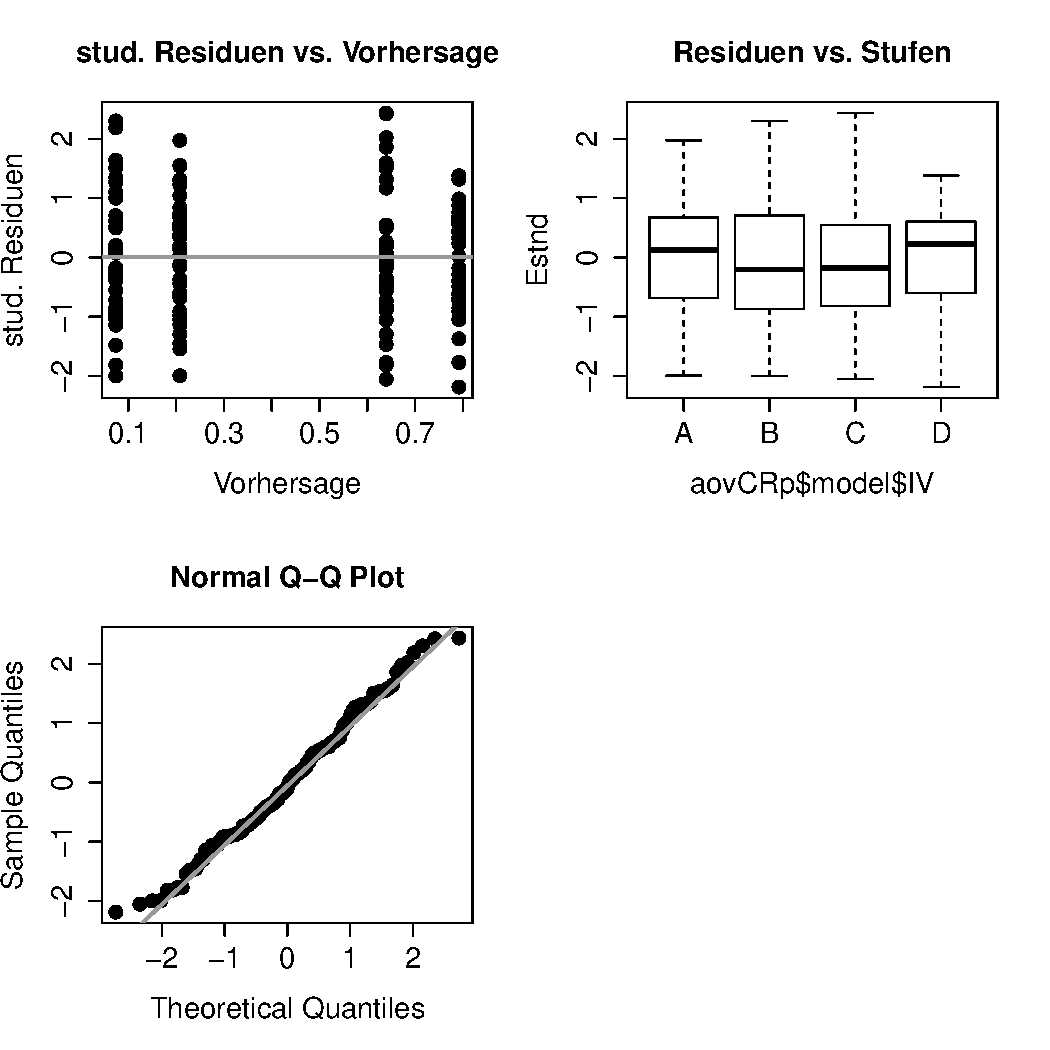
\includegraphics[width=12.5cm]{anovaDiag}
\vspace*{-0.5em}
\caption{Grafische Prüfung der Voraussetzungen für die einfaktorielle Varianzanalyse}
\label{fig:anovaDiag}
\end{figure}

%%%%%%%%%%%%%%%%%%%%%%%%%%%%%%%%%%%%%%%%%%%%%%%%%%%%%%%%%%%%%%%%%%
%%%%%%%%%%%%%%%%%%%%%%%%%%%%%%%%%%%%%%%%%%%%%%%%%%%%%%%%%%%%%%%%%%
\subsection{Einzelvergleiche (Kontraste)}
%%%%%%%%%%%%%%%%%%%%%%%%%%%%%%%%%%%%%%%%%%%%%%%%%%%%%%%%%%%%%%%%%%
%%%%%%%%%%%%%%%%%%%%%%%%%%%%%%%%%%%%%%%%%%%%%%%%%%%%%%%%%%%%%%%%%%

Ein Kontrast $\psi = \sum_{j} c_{j} \cdot \mu_{j}$ meint im Folgenden eine Linearkombination der $p$ Gruppenerwartungswerte $\mu_{j}$ mit den Koeffizienten $c_{j}$, wobei $1 \leq j \leq p$ sowie $\sum_{j} c_{j} = 0$ gilt. Solche Kontraste dienen einem spezifischen Vergleich zwischen den $p$ experimentellen Bedingungen. Über die Größe von $\psi$ lassen sich Hypothesen aufstellen (unter $\text{H}_{0}$ gilt meist $\psi_{0} = 0$), deren Test im Folgenden beschrieben wird (für eine formalere Darstellung s.\ Abschn.\ \ref{sec:multALMctr}).

%%%%%%%%%%%%%%%%%%%%%%%%%%%%%%%%%%%%%%%%%%%%%%%%%%%%%%%%%%%%%%%%%%
%%%%%%%%%%%%%%%%%%%%%%%%%%%%%%%%%%%%%%%%%%%%%%%%%%%%%%%%%%%%%%%%%%
\subsubsection{Beliebige a-priori Kontraste}
\label{sec:contrCRp}
%%%%%%%%%%%%%%%%%%%%%%%%%%%%%%%%%%%%%%%%%%%%%%%%%%%%%%%%%%%%%%%%%%
%%%%%%%%%%%%%%%%%%%%%%%%%%%%%%%%%%%%%%%%%%%%%%%%%%%%%%%%%%%%%%%%%%

\index{Varianzanalyse!Kontraste!a-priori}
Der Test beliebiger Kontraste lässt sich mit \lstinline!glht()!\index[func]{glht()@\lstinline{glht()}|textbf} (\emph{general linear hypothesis test}) aus dem Paket \lstinline!multcomp!\index[pack]{multcomp@\lstinline{multcomp}|textbf} \cite{Hothorn2008} durchführen. Hierfür ist zunächst der Kontrastvektor $\bm{c}$ aus den Koeffizienten $c_{j}$ der Linearkombination zu bilden.
\begin{lstlisting}
glht(<<aov-Modell>>, linfct=mcp(<<UV>>=<<Kontrastkoeffizienten>>),
     alternative=c("two.sided", "less", "greater"))
\end{lstlisting}

Als erstes Argument ist ein mit \lstinline!aov()! erstelltes Modell zu übergeben, dessen Gruppen einem spezifischen Vergleich unterzogen werden sollen. Dieser Vergleich kann mit dem \lstinline!linfct! Argument definiert werden, wozu die \lstinline!mcp()! Funktion dient. Diese erwartet ihrerseits eine Zuweisung der Form \lstinline!<<UV>>=<<Koeffizienten>>! als Argument. Dabei ist \lstinline!<<UV>>! der Name des Gruppierungsfaktors aus dem mit \lstinline!aov()! erstellten Modell (ohne Anführungszeichen) und \lstinline!<<Koeffizienten>>! eine zeilenweise aus (ggf.\ benannten) Kontrastvektoren zusammengestellte Matrix. Dabei muss jeder Koeffizient $c_{j}$ angegeben werden, also auch solche, die $0$ sind und somit nicht in die Linearkombination eingehen. Mit \lstinline!alternative! wird festgelegt, ob die $\text{H}_{1}$ gerichtet oder ungerichtet (\lstinline!"two.sided"!) ist. \lstinline!"less"! und \lstinline!"greater"! beziehen sich dabei auf die Reihenfolge $\psi < \psi_{0}$ bzw.\ $\psi > \psi_{0}$, wobei die Voreinstellung $\psi_{0} = 0$ ist.

\lstinline!summary(<<glht-Modell>>, test=adjusted("<<alpha-Adjustierung>>"))!\index[func]{summary()@\lstinline{summary()}} testet das Ergebnis auf Signifikanz. Das Argument \lstinline!test! erlaubt für den Test mehrerer Kontraste gleichzeitig, eine Methode zur\index{alpha-Adjustierung@$\alpha$-Adjustierung} $\alpha$-Adjustierung auszuwählen (vgl.\ \lstinline!?summary.glht!). Soll dies unterbleiben, ist \lstinline!test=adjusted("none")! zu setzen. Beim Aufstellen von Kontrasten ist zu beachten, dass die Reihenfolge der Gruppen durch die Reihenfolge der Faktorstufen bestimmt wird (Abschn.\ \ref{sec:facOrder}).

Im Beispiel soll zunächst nur der Vergleich des Mittels der ersten beiden gegen das Mittel der verbleibenden Gruppen getestet werden. Dabei sei $\psi_{0} = 0$ und unter $\text{H}_{1}$ $\psi < 0$.
\begin{lstlisting}
# Matrix der Kontrastkoeffizienten - hier nur eine Zeile
> cntrMat <- rbind("(A+B)-(C+D)"=c(1/2, 1/2, -1/2, -1/2))
> library(multcomp)                               # für glht()
> glhtRes <- glht(aovCRp, linfct=mcp(IV=cntrMat), alternative="less")
> summary(glhtRes)
Simultaneous Tests for General Linear Hypotheses
Multiple Comparisons of Means: User-defined Contrasts
Fit: aov(formula = DV ~ IV, data = dfCRp)
Linear Hypotheses:
                  Estimate  Std. Error  t value    Pr(<t)
(A+B)-(C+D) >= 0   -0.5746      0.1539   -3.735  0.000132 ***
\end{lstlisting}

Die Ausgabe führt den Namen des getesteten Kontrasts aus der Matrix der Kontrastkoeffizienten auf, gefolgt von der Schätzung $\hat{\psi}$, für die die Erwartungswerte in der Linearkombination durch die Gruppenmittelwerte ersetzt werden ($\hat{\psi} = \sum_{j} c_{j} \cdot M_{j}$). Es folgt der Standardfehler dieser Schätzung (\lstinline!Std. Error!), der Wert der $t$-Teststatistik (\lstinline!t value!) und der zugehörige $p$-Wert (\lstinline!Pr(<t)!).

Die Differenz $\hat{\psi} - \psi_{0}$ bildet den Zähler der Teststatistik $t$. Im Nenner wird die quadrierte Länge $\|\bm{c}\|^{2}$ des Kontrastvektors benötigt, für dessen Berechnung eine Gewichtung mit den Zellbesetzungen vorzunehmen ist. Das Produkt $\|\bm{c}\|^{2} \cdot \text{MS}_{w}$ der quadrierten Länge mit der mittleren Quadratsumme der Residuen aus der zugehörigen Varianzanalyse bildet den quadrierten Nenner der Teststatistik und stellt die Schätzung der Varianz des Kontrasts dar. Die Teststatistik ist im Fall von a-priori Kontrasten unter $\text{H}_{0}$ zentral $t$-verteilt mit den Freiheitsgraden der Quadratsumme der Residuen in der zugehörigen Varianzanalyse.
\begin{lstlisting}
> P       <- nlevels(dfCRp$IV)                    # Anzahl der Gruppen
> Mj      <- tapply(dfCRp$DV, dfCRp$IV, mean)     # Gruppenmittelwerte
> Nj      <- table(dfCRp$IV)                      # Gruppengrößen
> dfSSw   <- sum(Nj) - P                          # df von SS within
> SSw     <- sum((DV - ave(DV, IV, FUN=mean))^2)  # SS within
> MSw     <- SSw / dfSSw                          # MS within
> (psiHat <- sum(cntrMat[1, ] * Mj))              # Kontrastschätzung
[1] -0.5746347

> lenSq  <- sum(cntrMat[1, ]^2 / Nj)              # quadrierte Länge
> (tStat <- psiHat / sqrt(lenSq*MSw))             # Teststatistik t
[1] -3.734508

> (pVal <- pt(abs(tStat), dfSSw, lower.tail=FALSE)) # p-Wert einseitig
[1] 0.0001316091
\end{lstlisting}

Durch \lstinline!confint(<<glht-Modell>>)!\index[func]{confint()@\lstinline{confint()}} erhält man die Vertrauensintervalle der definierten $\psi$, die sich über \lstinline!plot(<<glht-Modell>>)! grafisch darstellen lassen.
\begin{lstlisting}
> confint(glhtRes)                    # einseitiges Konfidenzintervall
Simultaneous Confidence Intervals     # Ausgabe gekürzt ...
95% family-wise confidence level
Linear Hypotheses:
                  Estimate  lwr   upr    
(A+B)-(C+D) >= 0  -0.5746   -Inf  -0.3200

# obere Grenze des einseitigen 95%-Vertrauensintervalls für psi
> (tCrit <- qt(0.05, dfSSw, lower.tail=FALSE))    # krit. t-Wert eins.
[1] 1.65468

> (ciUp <- psiHat + tCrit*sqrt(lenSq*MSw))
[1] -0.3200264
\end{lstlisting}

Sollen mehrere Kontraste gleichzeitig getestet werden, verfügt die an das Argument \lstinline!linfct! übergebene Funktion \lstinline!mcp()! zum einen über Voreinstellungen für verschiedene Spezialfälle: Mit \lstinline!mcp(<<UV>>="Dunnett")! erhält man etwa alle $p-1$ paarweisen Vergleiche, in denen ein Gruppenerwartungswert gegen jenen der Referenzstufe (die erste Faktorstufe von \lstinline!<<UV>>!, s.\ Abschn.\ \ref{sec:facLabelOrder}) getestet wird. Analog erzeugt \lstinline!mcp(<<UV>>="Tukey")! alle Tests der paarweisen Gruppenvergleiche (s.\,u.). Zum anderen sind allgemeine Kontrast-Tests durch Zusammenstellung der zugehörigen Kontrastvektoren als (ggf.\ benannte) Zeilen einer Matrix möglich. Hier werden drei Kontraste ohne Adjustierung des $\alpha$-Niveaus gerichtet getestet.
\begin{lstlisting}
> cntrMat <- rbind("A-D"          =c(  1,   0,   0, -1),
+                  "1/3*(A+B+C)-D"=c(1/3, 1/3, 1/3, -1),
+                  "B-C"          =c(  0,   1,  -1,  0))

> glhtRes <- glht(aovCRp, linfct=mcp(IV=cntrMat), alternative="less")
> plot(glhtRes)               # Diagramm der Konfidenzintervalle
> (sumRes <- summary(glhtRes, test=adjusted("none")))
Simultaneous Tests for General Linear Hypotheses
Multiple Comparisons of Means: User-defined Contrasts
Fit: aov(formula = DV ~ IV, data = dfCRp)
Linear Hypotheses:
                    Estimate  Std. Error  t value   Pr(<t)
A-D >= 0             -0.5837      0.2160   -2.702  0.00383 **
1/3*(A+B+C)-D >= 0   -0.4845      0.1775   -2.729  0.00354 **
B-C >= 0             -0.5656      0.2192   -2.581  0.00539 **
\end{lstlisting}

Das Ergebnis lässt sich manuell prüfen.
\begin{lstlisting}
> psiHats <- cntrMat   %*% Mj               # Kontrastschätzungen
> lenSqs  <- cntrMat^2 %*% (1/Nj)           # quadrierte Längen
> tStats  <- psiHats / sqrt(lenSqs*MSw)     # Teststatistiken
> pVals   <- pt(abs(tStats), dfSSw, lower.tail=FALSE) # p-Werte eins.
> data.frame(psiHats, tStats, pVals)
                  psiHats     tStats        pVals
A-D            -0.5836704  -2.701783  0.003830077
1/3*(A+B+C)-D  -0.4845486  -2.729212  0.003539043
B-C            -0.5655991  -2.580620  0.005391977
\end{lstlisting}

%%%%%%%%%%%%%%%%%%%%%%%%%%%%%%%%%%%%%%%%%%%%%%%%%%%%%%%%%%%%%%%%%%
%%%%%%%%%%%%%%%%%%%%%%%%%%%%%%%%%%%%%%%%%%%%%%%%%%%%%%%%%%%%%%%%%%
\subsubsection{Beliebige post-hoc Kontraste nach Scheffé}
%%%%%%%%%%%%%%%%%%%%%%%%%%%%%%%%%%%%%%%%%%%%%%%%%%%%%%%%%%%%%%%%%%
%%%%%%%%%%%%%%%%%%%%%%%%%%%%%%%%%%%%%%%%%%%%%%%%%%%%%%%%%%%%%%%%%%

\index{Varianzanalyse!Kontraste!post-hoc (Scheffé)}
Beliebige Kontraste können auch im Anschluss an eine signifikante Varianzanalyse getestet werden. Die Varianzanalyse prüft implizit simultan alle möglichen Kontraste -- spezifische Hypothesen liegen also bei ihrer Anwendung nicht vor. Aus diesem Grund muss im Anschluss bei Einzeltests eine geeignete\index{alpha-Adjustierung@$\alpha$-Adjustierung} $\alpha$-Adjustierung vorgenommen werden, hier vorgestellt nach der Methode von Scheffé.\footnote{Für weitere vgl.\ \lstinline!?PostHocTest!\index[func]{PostHocTest()@\lstinline{PostHocTest()}} nach Laden des Pakets\index[pack]{DescTools@\lstinline{DescTools}} \lstinline!DescTools!.} Sie ist in\index[func]{ScheffeTest()@\lstinline{ScheffeTest()}} \lstinline!ScheffeTest()! aus dem Paket\index[pack]{DescTools@\lstinline{DescTools}} \lstinline!DescTools! implementiert.
\begin{lstlisting}
ScheffeTest(<<aov-Modell>>, which="<<UV>>", contrasts=<<Kontrastmatrix>>,
            conf.level=0.95)
\end{lstlisting}

Als erstes Argument ist die mit \lstinline!aov()! angepasste ANOVA zu übergeben. \lstinline!which! erwartet den Namen der UV, auf den sich die Kontraste beziehen, was hier im einfaktoriellen Fall optional ist. Für \lstinline!contrasts! ist die Kontrastmatrix anzugeben, wobei die Koeffizienten eines Kontrasts in einer Spalte stehen. Das Argument \lstinline!conf.level! legt die Breite des Konfidenzintervalls für $\psi$ fest. Hier sollen wieder die drei Kontraste des letzten Abschnitts getestet werden.
\begin{lstlisting}
> library(DescTools)                      # für ScheffeTest()
# transponiere cntrMat mit t(), damit Koeffizienten in Spalten stehen
> ScheffeTest(aovCRp, which="IV", contrasts=t(cntrMat))
Posthoc multiple comparisons of means : Scheffe Test
95% family-wise confidence level
Fit: aov(formula = DV ~ IV, data = dfCRp)
$IV
               diff     lwr.ci      upr.ci    pval
A-D      -0.5836704  -1.194230  0.02688944  0.0671 .
A,B,C-D  -0.4845486  -0.986326  0.01722875  0.0629 .
B-C      -0.5655991  -1.185034  0.05383580  0.0880 .
\end{lstlisting}

In der Ausgabe stehen die Ergebnisse für jeweils einen Kontrast in einer Zeile. Dies sind die Kontrastschätzung $\hat{\psi}$ in der Spalte \lstinline!diff!, das Konfidenzintervall für $\psi$ in den Spalten \lstinline!lwr.ci! und \lstinline!upr.ci! und schließlich der $p$-Wert in der Spalte \lstinline!pval!.

Bei der manuellen Kontrolle gilt zunächst alles bereits für a-priori Kontraste Ausgeführte. Lediglich die Wahl des kritischen Wertes weicht ab und ergibt sich zur $\alpha$-Adjustierung aus einer $F$-Verteilung. Dieser kritische Wert ist mit der quadrierten a-priori $t$-Teststatistik zu vergleichen -- die etwa in der von \lstinline!summary(glht(...))! zurückgegebenen Liste in der Komponente \lstinline!test$tstat! steht.
\begin{lstlisting}
> dfSSb  <- P-1                           # df von SS between
> (Fstat <- sumRes$test$tstat^2)          # quadrierte t-Teststatistik
     A-D  1/3*(A+B+C)-D       B-C
7.299631       7.448600  6.659600

# kritischer F-Wert für quadrierte t-Teststatistik
> (Fcrit <- dfSSb*qf(0.05, df1=dfSSb, df2=dfSSw, lower.tail=FALSE))
[1] 7.987706

# p-Wert einseitig
> (pVal <- pf(Fstat/dfSSb, dfSSb, dfSSw), lower.tail=FALSE)
       A-D  1/3*(A+B+C)-D         B-C
0.06706707     0.06294284  0.08801514
\end{lstlisting}

Die Wahl des kritischen Wertes erfolgte hier so, dass alle möglichen Kontraste zugelassen sind. Sollen sich die Kontraste dagegen nur auf einen Teil der Erwartungswerte beziehen (und damit aus einem Unterraum des $(p-1)$-dimensionalen Kontrastraumes stammen), kann der kritische Wert entsprechend anders gewählt werden. In diesem Fall erfolgt eine gleichzeitige\index{alpha-Adjustierung@$\alpha$-Adjustierung} $\alpha$-Adjustierung nur für Kontraste aus dem gewählten Unterraum, woraus ein etwas geringerer kritischer Wert resultiert. Ist $q$ mit $q < p$ die Anzahl der relevanten Gruppen, wäre der kritische $F$-Wert \lstinline!(q-1) * qf(1-0.05, q-1, dfSSw))!.

%%%%%%%%%%%%%%%%%%%%%%%%%%%%%%%%%%%%%%%%%%%%%%%%%%%%%%%%%%%%%%%%%%
%%%%%%%%%%%%%%%%%%%%%%%%%%%%%%%%%%%%%%%%%%%%%%%%%%%%%%%%%%%%%%%%%%
\subsubsection[{Paarvergleiche mit \texorpdfstring{$t$}{t}-Tests und \texorpdfstring{$\alpha$}{alpha}-Adjustierung}]{Paarvergleiche mit $\bm{t}$-Tests und $\bm{\alpha}$-Adjustierung}
\label{sec:pairwiseT}
%%%%%%%%%%%%%%%%%%%%%%%%%%%%%%%%%%%%%%%%%%%%%%%%%%%%%%%%%%%%%%%%%%
%%%%%%%%%%%%%%%%%%%%%%%%%%%%%%%%%%%%%%%%%%%%%%%%%%%%%%%%%%%%%%%%%%

\index{Varianzanalyse!Kontraste!paarweise $t$-Tests}
Taucht die spezifischere Frage auf, welche paarweisen Gruppenunterschiede vorliegen, besteht eine andere Herangehensweise in der Anwendung von ${p \choose 2} = \frac{p \, (p-1)}{2}$ $t$-Tests, um die Unterschiede jeweils zweier Gruppen auf Signifikanz zu prüfen. Das\index{alpha-Adjustierung@$\alpha$-Adjustierung} $\alpha$-Niveau ist zu adjustieren, da sonst mehrfach die Möglichkeit bestünde, denselben Fehler erster Art zu begehen und das tatsächliche $\alpha$-Niveau über dem nominellen läge. Anstatt mehrere solcher $t$-Tests manuell durchzuführen, lässt sich die Funktion \lstinline!pairwise.t.test()! nutzen, die alle möglichen Paarvergleiche testet und verschiedene Verfahren zur $\alpha$-Adjustierung\index[func]{pairwise.t.test()@\lstinline{pairwise.t.test()}} anbietet.
\begin{lstlisting}
pairwise.t.test(x=<<Vektor>>, g=<<Faktor>>, p.adjust.method="holm",
                paired=FALSE, pool.sd=!paired, alternative="two.sided")
\end{lstlisting}

Der Vektor \lstinline!x! muss die Messwerte enthalten, \lstinline!g! ist der zugehörige Faktor derselben Länge wie \lstinline!x!, der für jedes Element von \lstinline!x! die Gruppenzugehörigkeit codiert. Über das Argument \lstinline!p.adjust.method! wird die $\alpha$-Adjustierung festgelegt, als Methoden stehen u.\,a.\ jene nach Holm (Voreinstellung) und Bonferroni zur Auswahl, für weitere vgl.\ \lstinline!?p.adjust!. Ist von Varianzhomogenität auszugehen und daher \lstinline!pool.sd=TRUE! gesetzt, wird die Fehlerstreuung auf Basis aller, also nicht nur anhand der beiden beim jeweiligen $t$-Test beteiligten Gruppen bestimmt. Dies ist jedoch nur möglich, wenn keine abhängigen Stichproben vorliegen, was mit dem Argument \lstinline!paired! anzuzeigen ist. Für gerichtete Tests ist das Argument \lstinline!alternative! auf \lstinline!"less"! oder \lstinline!"greater"! zu setzen -- Voreinstellung ist \lstinline!"two.sided"! für ungerichtete Tests.
\begin{lstlisting}
> DV <- dfCRp$DV                              # Daten
> IV <- dfCRp$IV                              # Gruppierungsfaktor

# paarweise t-Tests mit alpha-Adjustierung nach Bonferroni
> pairwise.t.test(DV, IV, p.adjust.method="bonferroni")
Pairwise comparisons using t tests with pooled SD
data: DV and IV
   A       B       C
B  1.0000  -       -
C  0.2694  0.0647  -
D  0.0460  0.0088  1.0000
P value adjustment method: bonferroni
\end{lstlisting}

Die in Form einer Matrix ausgegebenen $p$-Werte für den Vergleich der jeweils in Zeile und Spalte angegebenen Gruppen berücksichtigen bereits die $\alpha$-Adjustierung, sie können also direkt mit dem gewählten Signifikanzniveau verglichen werden. Setzt man \lstinline!p.adjust.method="none"!, unterbleibt eine $\alpha$-Adjustierung, was zusammen mit \lstinline!pool.sd=FALSE! zu jenen Ergebnissen führt, die man mit separat durchgeführten zweiseitigen $t$-Tests ohne $\alpha$-Adjustierung erhalten hätte.

%%%%%%%%%%%%%%%%%%%%%%%%%%%%%%%%%%%%%%%%%%%%%%%%%%%%%%%%%%%%%%%%%%
%%%%%%%%%%%%%%%%%%%%%%%%%%%%%%%%%%%%%%%%%%%%%%%%%%%%%%%%%%%%%%%%%%
\subsubsection{Simultane Konfidenzintervalle nach Tukey}
\label{sec:tukey}
%%%%%%%%%%%%%%%%%%%%%%%%%%%%%%%%%%%%%%%%%%%%%%%%%%%%%%%%%%%%%%%%%%
%%%%%%%%%%%%%%%%%%%%%%%%%%%%%%%%%%%%%%%%%%%%%%%%%%%%%%%%%%%%%%%%%%

\index{Varianzanalyse!Kontraste!Tukey HSD}
\index[func]{TukeyHSD()@\lstinline{TukeyHSD()}}
Die Konstruktion simultaner Vertrauensintervalle nach Tukey für die paarweisen Differenzen der Gruppenerwartungswerte (Tukey \emph{honestly significant differences}) stellt eine weitere Möglichkeit dar, auf Unterschiede zwischen jeweils zwei Gruppen zu testen.
\begin{lstlisting}
TukeyHSD(<<aov-Objekt>>, which="<<Faktor>>", conf.level=0.95)
\end{lstlisting}

Als erstes Argument erwartet \lstinline!TukeyHSD()! ein von \lstinline!aov()! erstelltes Objekt. Wurde in ihm mehr als ein Faktor berücksichtigt, kann mit \lstinline!which! in Form eines Vektors aus Zeichenketten angegeben werden, welche dieser Faktoren für die Bildung von Gruppen herangezogen werden sollen. Über \lstinline!conf.level! wird die Breite des Vertrauensintervalls für die jeweilige Differenz zweier Erwartungswerte festgelegt.
\begin{lstlisting}
> (tHSD <- TukeyHSD(aovCRp))
Tukey multiple comparisons of means
95% family-wise confidence level
Fit: aov(formula = DV ~ IV, data = dfCRp)

$IV
           diff           lwr        upr      p adj
B-A  -0.1341170  -0.706534340  0.4383004  0.9292665
C-A   0.4314821  -0.122736070  0.9857003  0.1843991
D-A   0.5836704   0.022649650  1.1446911  0.0380018
C-B   0.5655991  -0.003576610  1.1347748  0.0521308
D-B   0.7177873   0.141985791  1.2935888  0.0079573
D-C   0.1521882  -0.405524534  0.7099010  0.8935478
\end{lstlisting}

Die Ausgabe umfasst für jeden Gruppenvergleich die beobachtete Mittelwertsdifferenz (\lstinline!diff!), ihr Vertrauensintervall (\lstinline!lwr!, \lstinline!upr!) sowie den zugehörigen $p$-Wert (\lstinline!p adj!). Auch \lstinline!glht()! aus dem Paket \lstinline!multcomp! kann alle paarweisen Gruppenvergleiche mit der $\alpha$-Adjustierung nach Tukey testen, indem das Argument \lstinline!linfct! auf \lstinline!mcp(<<UV>>="Tukey")! gesetzt wird.
\begin{lstlisting}
> library(multcomp)                             # für glht()
> tukey <- glht(aovCRp, linfct=mcp(IV="Tukey")) # Tukey Kontraste
> summary(tukey)                                # Tests ...
> confint(tukey)                              # Konfidenzintervalle ...
\end{lstlisting}

Die Ergebnisse lassen sich manuell nachvollziehen, wobei hier zu beachten ist, dass ungleiche Gruppengrößen vorliegen. Kritischer Wert und Verteilungsfunktion der Teststatistik sind mit \lstinline!qtukey()! bzw.\ \lstinline!ptukey()! zu berechnen.
\begin{lstlisting}
> Mj <- tapply(dfCRp$DV, dfCRp$IV, mean)        # Gruppenmittelwerte
> Nj <- table(dfCRp$IV)                         # Gruppengrößen

# alle paarweisen Mittelwertsdifferenzen
> diffMat <- outer(Mj, Mj, "-")
> (diffs  <- diffMat[lower.tri(diffMat)])
[1] -0.1341170 0.4314821 0.5836704 0.5655991 0.7177873 0.1521882

# Skalierungsfaktor: Wurzel aus Summe der Kehrwerte je zweier Nj
> NjMat  <- sqrt(outer(1/Nj, 1/Nj, "+"))
> NjFac  <- NjMat[lower.tri(NjMat)]
> qTs    <- abs(diffs) / (sqrt(MSw/2) * NjFac)    # Teststatistiken
> (pVals <- ptukey(qTs, P, dfSSw, lower.tail=FALSE))    # p-Werte
[1] 0.92926654 0.18439914 0.03800183 0.05213078 0.00795732 0.89354783

# halbe Breite Vertrauensintervall für paarweise Mittelwertsdifferenz
> tWidth <- qtukey(0.05, P, dfSSw, lower.tail=FALSE)*sqrt(MSw/2)*NjFac
> diffs - tWidth                # Vertrauensintervalle untere Grenzen
[1] -0.706534340 -0.122736070 0.022649650 -0.003576610
[5] 0.141985791 -0.405524534

> diffs + tWidth                # Vertrauensintervalle obere Grenzen
[1] 0.4383004 0.9857003 1.1446911 1.1347748 1.2935888 0.7099010
\end{lstlisting}

Die Konfidenzintervalle können grafisch veranschaulicht werden, indem das Ergebnis von \lstinline!TukeyHSD()! einem Objekt zugewiesen und dies an \lstinline!plot()!\index[func]{plot()@\lstinline{plot()}} übergeben wird (Abb.\ \ref{fig:tukey}). Die gestrichelt gezeichnete senkrechte Linie markiert die $0$ -- Intervalle, die die $0$ enthalten, entsprechen einem nicht signifikanten Paarvergleich.
\begin{lstlisting}
> plot(tHSD)
\end{lstlisting}

\begin{figure}[ht]
\centering
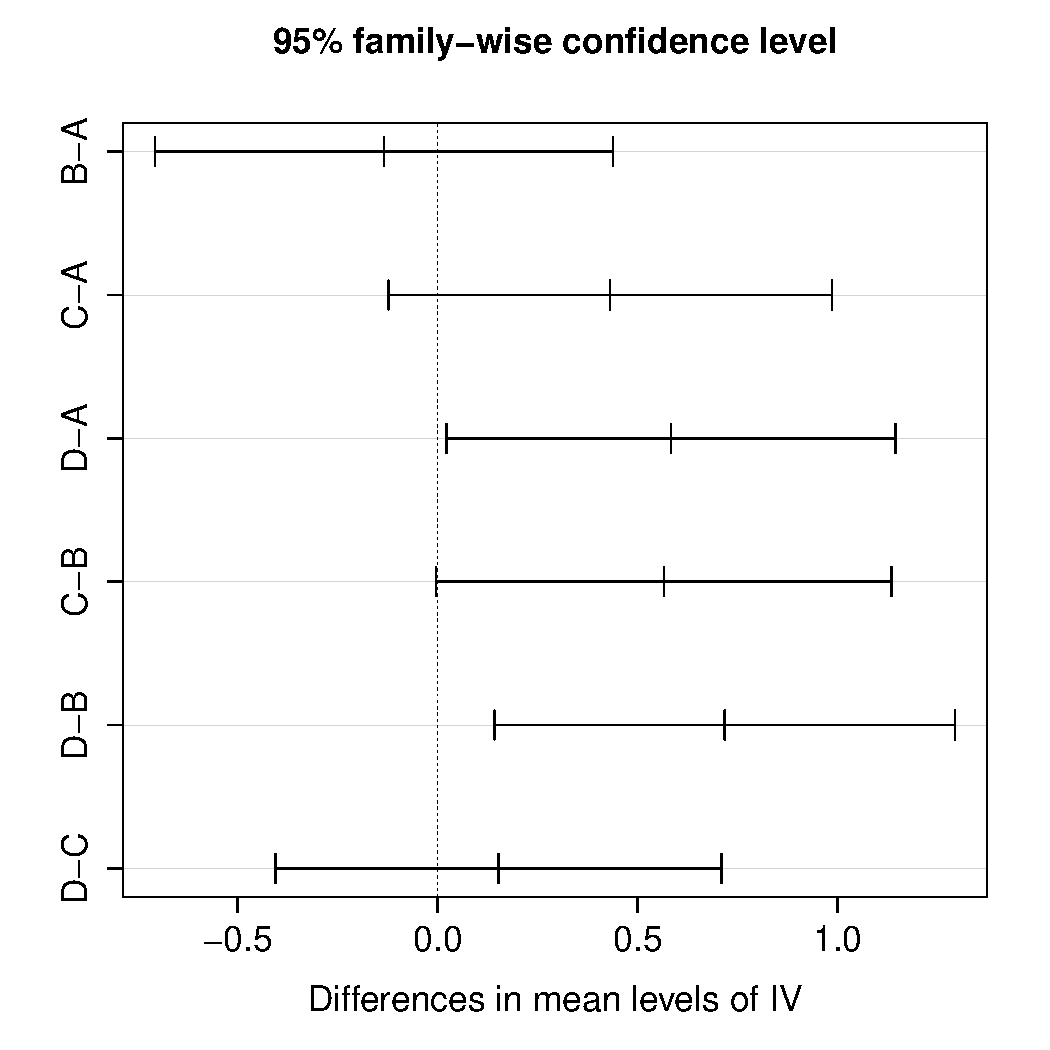
\includegraphics[width=8cm]{tukey}
\vspace*{-0.5em}
\caption{Grafische Darstellung simultaner Vertrauensintervalle nach Tukey}
\label{fig:tukey}
\end{figure}

%%%%%%%%%%%%%%%%%%%%%%%%%%%%%%%%%%%%%%%%%%%%%%%%%%%%%%%%%%%%%%%%%%
%%%%%%%%%%%%%%%%%%%%%%%%%%%%%%%%%%%%%%%%%%%%%%%%%%%%%%%%%%%%%%%%%%
\section[Einfaktorielle Varianzanalyse mit abhängigen Gruppen (RB-\texorpdfstring{$p$}{p})]{Einfaktorielle Varianzanalyse mit abhängigen Gruppen (RB-$\bm{p}$)}
\label{sec:RBp}
%%%%%%%%%%%%%%%%%%%%%%%%%%%%%%%%%%%%%%%%%%%%%%%%%%%%%%%%%%%%%%%%%%
%%%%%%%%%%%%%%%%%%%%%%%%%%%%%%%%%%%%%%%%%%%%%%%%%%%%%%%%%%%%%%%%%%

\index{Varianzanalyse!einfaktorielle!abhängige Gruppen (RB-$p$)}
In einem RB-$p$ Design werden in $p$ Bedingungen eines Gruppierungsfaktors (UV) abhängige Beobachtungen einer Zielgröße (AV) gemacht. Diese Situation verallgemeinert jene eines $t$-Tests für abhängige Stichproben auf mehr als zwei Gruppen. Jede Menge aus $p$ abhängigen Beobachtungen (eine aus jeder Bedingung) wird als \emph{Block} bezeichnet. Versuchsplanerisch ist zu beachten, dass im Fall der Messwiederholung die Reihenfolge der Beobachtungen für jede Person randomisiert wird, weswegen das Design unter \emph{randomized block design} firmiert. Bei gematchten Personen ist zunächst die Blockbildung so vorzunehmen, dass jeder Block $p$ Personen umfasst, die bzgl.\ relevanter Störvariablen homogen sind. Innerhalb jedes Blocks müssen daraufhin die Personen randomisiert den Bedingungen zugeordnet werden.

Im Vergleich zum CR-$p$ Design wirkt im Modell zum RB-$p$ Design ein systematischer Effekt mehr am Zustandekommen einer Beobachtung mit: Zusätzlich zum Effekt der Zugehörigkeit zu einer Bedingung ist dies der Blockeffekt\index{Varianzanalyse!Blockeffekt} aus der Zugehörigkeit einer Beobachtung zu einem Block. Im Gegensatz zum festen (\emph{fixed})\index{Varianzanalyse!fester Effekt} Gruppenfaktor stellt die Blockzugehörigkeit einen zufälligen (\emph{random})\index{Zufallseffekt|see{Varianzanalyse}}\index{Varianzanalyse!Random-Faktor} Faktor dar. Die Bezeichnungen leiten sich daraus ab, dass die Faktorstufen inhaltlich bedeutsam sind, durch den Versuchsleiter reproduzierbar festgelegt werden und eine Generalisierung der Ergebnisse über diese Stufen hinaus nicht erfolgt. Die vorliegenden Ausprägungen der Blockzugehörigkeit (im Fall der Messwiederholung die Personen selbst) sind dagegen selbst nicht bedeutsam. Stattdessen sind sie nicht kontrollierte Realisierungen einer Zufallsvariable im statistischen Sinn. Dies erlaubt es den Ergebnissen, über die tatsächlich realisierten Werte hinaus verallgemeinert werden zu können.

%%%%%%%%%%%%%%%%%%%%%%%%%%%%%%%%%%%%%%%%%%%%%%%%%%%%%%%%%%%%%%%%%%
%%%%%%%%%%%%%%%%%%%%%%%%%%%%%%%%%%%%%%%%%%%%%%%%%%%%%%%%%%%%%%%%%%
\subsection{Univariat formuliert auswerten und Effektstärke schätzen}
%%%%%%%%%%%%%%%%%%%%%%%%%%%%%%%%%%%%%%%%%%%%%%%%%%%%%%%%%%%%%%%%%%
%%%%%%%%%%%%%%%%%%%%%%%%%%%%%%%%%%%%%%%%%%%%%%%%%%%%%%%%%%%%%%%%%%

Für die Durchführung der Varianzanalyse ergeben sich wichtige Änderungen im Vergleich zum CR-$p$ Design. Zunächst sind die statistischen Voraussetzungen andere: Die jeweils pro Block erhobenen Daten müssen, als Zufallsvektoren aufgefasst, gemeinsam normalverteilt sein. Darüber hinaus muss Zirkularität\index{Varianzanalyse!Zirkularität|textbf} gelten (Abschn.\ \ref{sec:sphericity}). Für die Durchführung des Tests mit \lstinline!aov()! muss der Datensatz so strukturiert sein, dass die Messwerte eines Blocks aus verschiedenen Messzeitpunkten in separaten Zeilen stehen\index{Datensatz!Long-Format} (Long-Format, s.\ Abschn.\ \ref{sec:reshape}). Der Messzeitpunkt muss mit einem Objekt der Klasse \lstinline!factor! codiert werden. Weiterhin muss es eine Variable geben, die codiert, von welcher Person, bzw.\ allgemeiner aus welchem Block ein Messwert stammt. Dieser Blockbildungsfaktor sei im Folgenden als \lstinline!<<Block>>! bezeichnet und muss ein Objekt der Klasse \lstinline!factor! sein.\footnote{Bei Verwendung von \lstinline!reshape()! werden sowohl die Blockzugehörigkeit als auch der Messzeitpunkt als numerischer Vektor codiert. Beide Variablen sind deshalb manuell in Faktoren umzuwandeln.}
\begin{lstlisting}
aov(<<AV>> ~ <<UV>> + Error(<<Block>>/<<UV>>), data=<<Datensatz>>)
\end{lstlisting}

Weil die Fehlerstruktur der Messwerte blockweise Abhängigkeiten aufweist, ändert sich die Modellformel in den Aufrufen von \lstinline!aov()! dahingehend, dass explizit anzugeben ist, aus welchen additiven Komponenten sich die Quadratsumme innerhalb der Gruppen zusammensetzt. Im RB-$p$ Design drückt \lstinline!Error(<<Block>>/<<UV>>)!\index[func]{Error()@\lstinline{Error()}} aus, dass \lstinline!<<Block>>! in \lstinline!<<UV>>! verschachtelt ist und der durch die Variation der UV entstehende Effekt in der AV jeweils innerhalb der durch \lstinline!<<Block>>! definierten Blöcke analysiert werden muss.\footnote{Ausgeschrieben lautet der Term \lstinline!Error(<<Block>> + <<Block>>:<<UV>>)!. Dies sind die beiden Effekte, deren Quadratsummen sich zur Quadratsumme innerhalb der Gruppen addieren -- also zur Quadratsumme der Residuen einer CR-$p$ ANOVA, die keinen Effekt von \lstinline!<<Block>>! berücksichtigt (\lstinline!anova(lm(DV ~ IV, data=dfRBpL))!).}
\begin{lstlisting}
> N     <- 10                               # Zellbesetzung
> P     <- 4                                # Anzahl UV-Stufen
> id    <- factor(rep(1:N, times=P))        # Blockzugehörigkeit
> IV    <- factor(rep(1:P, each=N))         # Intra-Gruppen Faktor
> DV_t1 <- round(rnorm(N, -0.3, 1), 2)      # AV zu t1
> DV_t2 <- round(rnorm(N, -0.2, 1), 2)      # AV zu t2
> DV_t3 <- round(rnorm(N,  0.1, 1), 2)      # AV zu t3
> DV_t4 <- round(rnorm(N,  0.4, 1), 2)      # AV zu t4
> DV    <- c(DV_t1, DV_t2, DV_t3, DV_t4)    # Gesamt-Daten

> dfRBpL <- data.frame(id, IV, DV)          # Datensatz Long-Format
> aovRBp <- aov(DV ~ IV + Error(id/IV), data=dfRBpL)
> summary(aovRBp)
Error: id
           Df  Sum Sq  Mean Sq  F value  Pr(>F)
Residuals   9  15.115   1.6795

Error: id:IV
           Df  Sum Sq  Mean Sq  F value   Pr(>F)
IV          3  12.569   4.1895   3.9695  0.01823 *
Residuals  27  28.496   1.0554
\end{lstlisting}

Die beim Test eines Effekts jeweils verwendete Quelle der Fehlervarianz wird durch die \lstinline!Error: <<Effekt>>! Überschriften kenntlich gemacht, ihre Quadratsumme findet sich in der Zeile \lstinline!Residuals!. Im RB-$p$ Design wird die Quadratsumme des festen Effekts (\lstinline!IV!) gegen die Quadratsumme der Interaktion von festem und Random-Faktor getestet (\lstinline!Error: id:IV!). Dies wird auch deutlich, wenn die Daten eines RB-$p$ Designs mit einer zweifaktoriellen Varianzanalyse im CRF-$pq$ Design analysiert werden (Abschn.\ \ref{sec:CRFpq}), wobei der Random- und der feste Faktor jeweils die Rolle einer UV einnehmen:
\begin{lstlisting}
> anova(lm(DV ~ id + IV + id:IV, data=dfRBpL))
Analysis of Variance Table
           Df  Sum Sq  Mean Sq  F value  Pr(>F)
id          9  15.115   1.6795
IV          3  12.569   4.1895
id:IV      27  28.496   1.0554
Residuals   0   0.000
\end{lstlisting}

Die sich in dieser Varianzanalyse ergebende Quadratsumme der Interaktion beider UVn (\lstinline!id:IV!) ist identisch zu jener der Residuen beim Test des festen Effekts im RB-$p$ Design. Analoges gilt für den Effekt der Variable \lstinline!id!, dessen Quadratsumme gleich der ersten Residual-Quadratsumme im RB-$p$ Design ist. Die Effekt-Quadratsumme von \lstinline!IV! ist in beiden Varianzanalysen notwendigerweise identisch. Da aus jedem Block nur eine Beobachtung pro Stufe von \lstinline!IV! vorliegt, beträgt im CRF-$pq$ Design die Zellbesetzung $1$. Deshalb kann es keine Abweichungen zum Zellmittelwert geben (\lstinline!Residuals! beträgt $0$) -- der Vorhersage des Modells mit beiden Haupteffekten und Interaktionseffekt.

%%%%%%%%%%%%%%%%%%%%%%%%%%%%%%%%%%%%%%%%%%%%%%%%%%%%%%%%%%%%%%%%%%
%%%%%%%%%%%%%%%%%%%%%%%%%%%%%%%%%%%%%%%%%%%%%%%%%%%%%%%%%%%%%%%%%%
\subsubsection{Manuelle Kontrolle}
%%%%%%%%%%%%%%%%%%%%%%%%%%%%%%%%%%%%%%%%%%%%%%%%%%%%%%%%%%%%%%%%%%
%%%%%%%%%%%%%%%%%%%%%%%%%%%%%%%%%%%%%%%%%%%%%%%%%%%%%%%%%%%%%%%%%%

Die Ergebnisse lassen sich manuell prüfen, wobei nach dem Bilden der blockweise zentrierten Daten wie im CR-$p$ Design vorgegangen werden kann. Lediglich die Freiheitsgrade der Fehler unterscheiden sich, zudem ist das Gesamtmittel der zentrierten Daten $0$.
\begin{lstlisting}
# für Quadratsummen: jeden Wert durch zugehöriges Mittel ersetzen
> MiL   <- ave(DV, id, FUN=mean)            # Block
> MjL   <- ave(DV, IV, FUN=mean)            # Messzeitpunkt
> DVctr <- DV - MiL                         # blockweise zentrierte AV
> MjCtr <- tapply(DVctr, IV, mean)          # Messzeitpunkt-Mittel
> SSb   <- sum(N * MjCtr^2)                 # Quadratsumme UV
> M     <- mean(DV)                         # Gesamtmittel

# Interaktion Block:UV, alternativ analog zu SSb im CR-p Design
# IDxIV <- DVctr - ave(DVctr, IV, FUN=mean)
> IDxIV <- DV - MiL - MjL + M               # Interaktion
> SSE   <- sum(IDxIV^2)                     # Quadratsumme Residuen
> dfSSb <- P-1                              # Freiheitsgrade UV
> dfSSE <- (N-1) * (P-1)                    # Freiheitsgrade Fehler
> (MSb  <- SSb / dfSSb)                     # mittlere QS UV
[1] 4.189542

> (MSE <- SSE / dfSSE)                      # mittlere QS Residuen
[1] 1.055424

> (Fval <- MSb / MSE)                       # Teststatistik F-Wert
[1] 3.969535

> (pVal <- pf(Fval, dfSSb, dfSSE, lower.tail=FALSE))  # p-Wert
[1] 0.01823255
\end{lstlisting}

%%%%%%%%%%%%%%%%%%%%%%%%%%%%%%%%%%%%%%%%%%%%%%%%%%%%%%%%%%%%%%%%%%
%%%%%%%%%%%%%%%%%%%%%%%%%%%%%%%%%%%%%%%%%%%%%%%%%%%%%%%%%%%%%%%%%%
\subsubsection{Effektstärke schätzen}
%%%%%%%%%%%%%%%%%%%%%%%%%%%%%%%%%%%%%%%%%%%%%%%%%%%%%%%%%%%%%%%%%%
%%%%%%%%%%%%%%%%%%%%%%%%%%%%%%%%%%%%%%%%%%%%%%%%%%%%%%%%%%%%%%%%%%

\index{Varianzanalyse!Effektstärke}
\index{etaSq@$\hat{\eta}^{2}$ (Effektstärke)}
Als Maß für die Effektstärke kann das generalisierte $\eta_{g}^{2}$ herangezogen werden, zu dessen Schätzung $\hat{\eta}_{g}^{2}$ die Effekt-Quadratsumme an der Summe von ihr selbst mit allen Residual-Quadratsummen relativiert wird. Die Berechnung -- inkl.\ des hier identischen einfachen $\hat{\eta}^{2}$ und des partiellen $\hat{\eta}_{p}^{2}$ -- übernimmt\index[func]{EtaSq()@\lstinline{EtaSq()}} \lstinline!EtaSq(<<aov-Objekt>>)! aus dem Paket\index[pack]{DescTools@\lstinline{DescTools}} \lstinline!DescTools!. Alternativ dient auch die Intraklassenkorrelation $ICC1$ als Maß der Effektstärke in RB-$p$ Designs (Abschn.\ \ref{sec:irr}).
\begin{lstlisting}
> library(DescTools)                        # für EtaSq()
> EtaSq(aovRBp, type=1)
     eta.sq  eta.sq.part  eta.sq.gen
IV  0.22372    0.3060661     0.22372
\end{lstlisting}

Da von \lstinline!summary(<<aov-Modell>>)! zurückgegebene Objekte eine recht verschachtelte Struktur besitzen, lassen sich die Quadratsummen zur manuellen Kontrolle hier leichter aus dem von \lstinline!anova(<<lm-Modell>>)! erzeugten Datensatz extrahieren.
\begin{lstlisting}
> anRes <- anova(lm(DV ~ IV*id, data=dfRBpL))

# Residual-Quadratsummen
> SSEid   <- anRes["id",    "Sum Sq"]
> SSEIVid <- anRes["IV:id", "Sum Sq"]
> SSb     <- anRes["IV", "Sum Sq"]          # Effekt-QS
> (pEtaSq <- SSb / (SSb + SSEIVid))         # partielles eta^2
[1] 0.3060661

> SSEtot  <- SSEid + SSEIVid
> (gEtaSq <- SSb / (SSb + SSEtot))          # generalisiertes eta^2
[1] 0.22372
\end{lstlisting}

%%%%%%%%%%%%%%%%%%%%%%%%%%%%%%%%%%%%%%%%%%%%%%%%%%%%%%%%%%%%%%%%%%
%%%%%%%%%%%%%%%%%%%%%%%%%%%%%%%%%%%%%%%%%%%%%%%%%%%%%%%%%%%%%%%%%%
\subsection{Zirkularität der Kovarianzmatrix prüfen}
\label{sec:sphericity}
%%%%%%%%%%%%%%%%%%%%%%%%%%%%%%%%%%%%%%%%%%%%%%%%%%%%%%%%%%%%%%%%%%
%%%%%%%%%%%%%%%%%%%%%%%%%%%%%%%%%%%%%%%%%%%%%%%%%%%%%%%%%%%%%%%%%%

\index{Varianzanalyse!Zirkularität}
\index{Zirkularität|see{Varianzanalyse}}
Die Gültigkeit der dargestellten Varianzanalyse für Daten aus einem RB-$p$ Design hängt davon ab, ob neben den anderen Voraussetzungen auch die Annahme von Zirkularität der theoretischen Kovarianzmatrix der AV in den einzelnen Gruppen gilt. Sie ist gegeben, wenn alle aus je zwei unterschiedlichen Variablen gebildeten Differenzvariablen dieselbe theoretische Varianz besitzen.\footnote{Dies ist bei nur zwei Gruppen immer der Fall.} Ein Test auf Zirkularität ist der von Mauchly (Abschn.\ \ref{sec:AnovaRBp}, \ref{sec:RBpMX}).

\index{Varianzanalyse!Zirkularität!$\varepsilon$-Korrektur|textbf}
Für Situationen ohne gegebene Zirkularität sollen Korrekturformeln verhindern, dass in der Varianzanalyse die tatsächliche Wahrscheinlichkeit eines Fehlers erster Art höher als das nominelle $\alpha$-Niveau ist. Ist $p$ die Anzahl der Gruppen, besteht die Korrektur in der Multiplikation der Zähler- und Nenner-Freiheitsgrade des getesteten $F$-Bruchs mit einem Skalar $\varepsilon$, für den $\frac{1}{p-1} \leq \varepsilon \leq 1$ gilt. $\varepsilon$ ist genau dann $1$, wenn die theoretische Kovarianzmatrix zirkulär ist, andernfalls schwankt $\varepsilon$ in Abhängigkeit vom Ausmaß der Abweichung von Zirkularität. Um die zugehörige Schätzung $\hat{\varepsilon}$ zu berechnen, sind u.\,a.\ die Methoden von Box (auch als Greenhouse-Geisser-Korrektur bezeichnet) sowie von Huynh und Feldt anwendbar. Es folgt eine manuelle Berechnung dieser Schätzungen, s.\ Abschn.\ \ref{sec:AnovaRBp} für die automatische Berechnung.
\begin{lstlisting}
# Schätzung von epsilon nach Greenhouse & Geisser
> DVmat  <- cbind(DV_t1, DV_t2, DV_t3, DV_t4)   # Daten im Wide-Format
> N      <- nrow(DVmat)         # Anzahl Beobachtungen
> S      <- var(DVmat)          # empirische Kovarianzmatrix
> P      <- nrow(S)             # Anzahl Variablen (UV-Stufen)
> mdS    <- mean(diag(S))       # Mittelwert der Diagonalelemente von S
> mS     <- mean(S)             # Mittelwert aller Elemente von S
> mSr    <- rowMeans(S)         # Zeilenmittelwerte von S
> num    <- P^2 * (mdS-mS)^2                                  # Zähler
> den    <- (P-1)*(sum(S^2) - 2*P*sum(mSr^2) + P^2*mS^2)      # Nenner
> (epsGG <- num/den)
[1] 0.786984

# Schätzung von epsilon nach Huynh & Feldt
> dfId   <- N-1                 # df Blockeffekt = df Fehler
> (epsHF <- ((dfId+1)*(P-1)*epsGG - 2) / ((P-1)*(dfId - (P-1)*epsGG)))
[1] 1.084971

# setze epsilon nach Hyhnh & Feldt auf 1, wenn es größer ist
> epsHF <- min(c(1, epsHF))

# Multiplikation der Freiheitsgrade mit epsilon & Vergleich der p-Werte
# p-Wert Greenhouse & Geisser
> (pEpsGG <- pf(Fval, dfSSb*epsGG, dfSSE*epsGG, lower.tail=FALSE))
[1] 0.02875036

# p-Wert Huynh & Feldt
> (pEpsHF <- pf(Fval, dfSSb*epsHF, dfSSE*epsHF, lower.tail=FALSE))
[1] 0.01823255
\end{lstlisting}

Im Beispiel bringt die Korrektur der Freiheitsgrade einen größeren $p$-Wert mit sich, wobei dies nicht in jeder Situation der Fall sein muss. Die Korrektur nach Greenhouse und Geisser gilt in Bereichen oberhalb von $0.9$ als etwas zu konservativ. Dies ist nicht der Fall für die Korrektur nach Huynh und Feldt, deren Schätzung aber auch zu Werten größer als $1$ führen kann. In diesen Fällen sollte die Schätzung auf $1$ gesetzt werden. Soll dagegen konservativ getestet werden, ist die Schätzung $\hat{\varepsilon}$ pauschal auf das theoretische Minimum $\frac{1}{p-1}$ zu setzen.

Im vorangehenden Abschnitt wurde bereits die Quadratsumme der Interaktion \lstinline!<<Block>>:<<UV>>! manuell berechnet, die als Quadratsumme der Residuen beim Test des festen Effekts dient. Hier kann zur Berechnung von $\hat{\varepsilon}$ nach Greenhouse und Geisser deshalb auch die etwas einfachere Formel verwendet werden, die auf der Kovarianzmatrix der Residuen basiert.
\begin{lstlisting}
# dem Datensatz Interaktion als neue Variable hinzufügen
> dfRBpL <- cbind(dfRBpL, IDxIV)

# Residuen als Matrix im Wide-Format extrahieren
> errMat <- data.matrix(unstack(dfRBpL, IDxIV ~ IV))
> Serr   <- cov(errMat)                 # Kovarianzmatrix der Residuen
> (epsGG <- (1/(P-1)) * sum(diag(Serr))^2 / sum(Serr^2)) # epsilon G&G
[1] 0.786984
\end{lstlisting}

%%%%%%%%%%%%%%%%%%%%%%%%%%%%%%%%%%%%%%%%%%%%%%%%%%%%%%%%%%%%%%%%%%
%%%%%%%%%%%%%%%%%%%%%%%%%%%%%%%%%%%%%%%%%%%%%%%%%%%%%%%%%%%%%%%%%%
\subsection{Multivariat formuliert auswerten mit \texttt{Anova()}}
\label{sec:AnovaRBp}
%%%%%%%%%%%%%%%%%%%%%%%%%%%%%%%%%%%%%%%%%%%%%%%%%%%%%%%%%%%%%%%%%%
%%%%%%%%%%%%%%%%%%%%%%%%%%%%%%%%%%%%%%%%%%%%%%%%%%%%%%%%%%%%%%%%%%

\index{Varianzanalyse!einfaktorielle!abhängige Gruppen (RB-$p$)}
\lstinline!Anova()!\index[func]{Anova()@\lstinline{Anova()}|textbf} aus dem \lstinline!car!\index[pack]{car@\lstinline{car}} Paket erlaubt die Durchführung von Varianzanalysen mit Messwiederholung, wobei sowohl die bereits beschriebene univariate wie auch eine multivariate Auswertung möglich ist (Abschn.\ \ref{sec:multRBp}). Ein Vorteil besteht darin, mit einer leicht nachvollziehbaren Syntax direkt anzugeben, bzgl.\ welcher Faktoren abhängige Messungen vorliegen. Weiterhin berechnet \lstinline!Anova()! den Mauchly-Test\index{Varianzanalyse!Zirkularität!Mauchly-Test}\index{Mauchly-Test} auf Zirkularität und die Schätzungen $\hat{\varepsilon}$ als Maß für die Abweichung der Kovarianzmatrix von Zirkularität mit den Methoden von Greenhouse und Geisser sowie von Huynh und Feldt\index{Varianzanalyse!Zirkularität!$\varepsilon$-Korrektur}
 samt der korrigierten $p$-Werte.
\begin{lstlisting}
Anova(<<lm-Modell>>, type=c("II", "III"), idata=<<Datensatz>>,
      idesign=<<Modellformel>>)
\end{lstlisting}

Zunächst ist ein mit \lstinline!lm()! erstelltes lineares Modell zu übergeben, das bei abhängigen Designs multivariat formuliert werden muss -- statt einer einzelnen gibt es also mehrere Zielgrößen. In der Modellformel \lstinline!<<AV>> ~ <<UV>>! werden dazu auf der linken Seite der \lstinline!~! die Daten der Zielgröße als Matrix zusammengefügt, wobei jede Spalte die Werte der Zielgröße in einer Gruppe (z.\,B.\ zu einem Messzeitpunkt) beinhaltet. Auf der rechten Seite der \lstinline!~! werden die Zwischen-Gruppen Faktoren aufgeführt, wenn es sich um ein gemischtes Design handelt (Abschn.\ \ref{sec:SPFpq}). Liegt ein reines Intra-Gruppen Design vor, ist hier nur die Konstante \lstinline!1! anzugeben. Sind etwa die Werte einer an denselben Personen gemessenen Zielgröße zu drei Messzeitpunkten in den Variablen \lstinline!t1!, \lstinline!t2! und \lstinline!t3! des Datensatzes \lstinline!myDf! gespeichert, lautet das Modell \lstinline!lm(cbind(t1, t2, t3) ~ 1, data=myDf)!.

Mit \lstinline!type! kann der Quadratsummen-Typ beim Test festgelegt werden (Typ II oder Typ III, Abschn.\ \ref{sec:ssTypes}), der im mehrfaktoriellen Fall mit ungleichen Zellbesetzungen relevant ist. Die Argumente \lstinline!idata! und \lstinline!idesign! dienen der Spezifizierung der Intra-Gruppen Faktoren. Hierfür erwartet \lstinline!idata! einen Datensatz, der die Struktur der als Matrix zusammengefassten Daten der Zielgröße beschreibt. Im RB-$p$ Design beinhaltet \lstinline!idata! eine Variable der Klasse \lstinline!factor!, die die Stufen des Intra-Gruppen Faktors codiert. In jeder Zeile von \lstinline!idata! gibt dieser Faktor an, aus welcher Bedingung die zugehörige Spalte der Datenmatrix stammt. Im obigen Design mit vier Messzeitpunkten könnte das Argument \lstinline!idata! damit \lstinline!data.frame(IV=factor(1:3))! lauten -- die erste Spalte der Datenmatrix entspricht der ersten Zeile von \lstinline!idata!, also der Bedingung \lstinline!1!, usw. Unter \lstinline!idesign! wird eine Modellformel mit den Intra-Gruppen Vorhersagetermen auf der rechten Seite der \lstinline!~! angegeben, die linke Seite bleibt leer. Im RB-$p$ Design lautet das Argument also \lstinline!idesign=~IV!.
\begin{lstlisting}
# Datensatz im Wide-Format
> dfRBpW <- data.frame(DV_t1, DV_t2, DV_t3, DV_t4)

# Zwischen-Gruppen Design (hier kein Zwischen-Gruppen Faktor)
> fitRBp <- lm(cbind(DV_t1, DV_t2, DV_t3, DV_t4) ~ 1, data=dfRBpW)
> inRBp  <- data.frame(IV=gl(P, 1))             # Intra-Gruppen Design
> library(car)                                  # für Anova()
> AnovaRBp <- Anova(fitRBp, idata=inRBp, idesign=~IV)
\end{lstlisting}

Der Test des Modells erfolgt mit\index[func]{summary()@\lstinline{summary()}} \lstinline!summary()!. Als Besonderheit bei der Anwendung auf ein von \lstinline!Anova()! erzeugtes Modell kann mit den Argumenten \lstinline!univariate! und \lstinline!multivariate! angegeben werden, ob die univariaten und multivariaten Kennwerte berechnet werden sollen.
\begin{lstlisting}
> summary(AnovaRBp, multivariate=FALSE, univariate=TRUE)        # ...
\end{lstlisting}

\lstinline!Anova()! setzt hier voraus, dass die Anzahl der Freiheitsgrade des Blockeffekts ($n-1$) mindestens so groß ist wie jene des Intra-Gruppen Effekts ($p-1$). Es müssen also mindestens so viele Blöcke wie Bedingungen vorhanden sein. Ist dies nicht der Fall, kann für die automatische Berechnung der $\hat{\varepsilon}$-Korrekturen wie im folgenden Abschnitt beschrieben auf \lstinline!anova()! ausgewichen werden.

%%%%%%%%%%%%%%%%%%%%%%%%%%%%%%%%%%%%%%%%%%%%%%%%%%%%%%%%%%%%%%%%%%
%%%%%%%%%%%%%%%%%%%%%%%%%%%%%%%%%%%%%%%%%%%%%%%%%%%%%%%%%%%%%%%%%%
\subsection{Multivariat formuliert auswerten mit \texttt{anova()}}
\label{sec:RBpMX}
%%%%%%%%%%%%%%%%%%%%%%%%%%%%%%%%%%%%%%%%%%%%%%%%%%%%%%%%%%%%%%%%%%
%%%%%%%%%%%%%%%%%%%%%%%%%%%%%%%%%%%%%%%%%%%%%%%%%%%%%%%%%%%%%%%%%%

Die Auswertung des RB-$p$ Designs in multivariater Formulierung ist auch mit der bereits bekannten \lstinline!anova()!\index[func]{anova()@\lstinline{anova()}} Funktion möglich, die es jedoch anders als \lstinline!Anova()! erlaubt, dass weniger Blöcke als Gruppen vorliegen. Wie bei \lstinline!Anova()! muss das erste Argument ein mit \lstinline!lm()! multivariat formuliertes Modell sein und die AV-Struktur in Form des Datensatzes \lstinline!idata! angegeben werden. Die Ergebnisse sind identisch zur univariat formulierten Auswertung, wenn das Argument \lstinline!test="Spherical"! gesetzt wird.\footnote{\label{ftn:spherical}Bei der multivariaten Formulierung des Modells wird intern aufgrund der generischen \lstinline!anova()! Funktion automatisch \lstinline!anova.mlm()! verwendet, ohne dass dies explizit angegeben werden muss (Abschnitt \ref{sec:funcGeneric}). Ohne das Argument \lstinline!test="Spherical"! wird multivariat getestet (Abschn.\ \ref{sec:multRBp}).} $\varepsilon$ wird mit den Methoden von Greenhouse und Geisser sowie von Huynh und Feldt\index{Varianzanalyse!Zirkularität!$\varepsilon$-Korrektur} geschätzt und samt der korrigierten $p$-Werte ausgegeben.

Die Angabe des zu testenden Effekts erfolgt mit den Argumenten \lstinline!M! und \lstinline!X! in Form eines Modellvergleichs. \lstinline!M! spezifiziert als rechte Seite einer Modellformel das umfassendere Intra-Gruppen Modell mit dem zu testenden Effekt, \lstinline!X! analog das eingeschränkte Intra-Gruppen Modell ohne diesen Effekt (Abschn.\ \ref{sec:regrCmp}, \ref{sec:anova}, \ref{sec:multALMmodCmp} sowie \citeNP{Dalgaard2007}). Die Kennwerte des von \lstinline!X! zu \lstinline!M! hinzugenommenen Effekts stehen in der Ausgabe in der Zeile \lstinline!(Intercept)!.
\begin{lstlisting}
> anova(fitRBp, M=~IV, X=~1, idata=inRBp, test="Spherical")     # ...
\end{lstlisting}

\index{Varianzanalyse!Zirkularität!Mauchly-Test}\index{Mauchly-Test}
Der Mauchly-Test auf Zirkularität wird mit der Funktion \index[func]{mauchly.test()@\lstinline{mauchly.test()}|textbf} \lstinline!mauchly.test()! durchgeführt, deren Argumente dieselben wie beim obigen Aufruf von \lstinline!anova()! sind.
\begin{lstlisting}
> mauchly.test(fitRBp, M=~IV, X=~1, idata=inRBp)                # ...
\end{lstlisting}

%%%%%%%%%%%%%%%%%%%%%%%%%%%%%%%%%%%%%%%%%%%%%%%%%%%%%%%%%%%%%%%%%%
%%%%%%%%%%%%%%%%%%%%%%%%%%%%%%%%%%%%%%%%%%%%%%%%%%%%%%%%%%%%%%%%%%
\subsection{Einzelvergleiche und alternative Auswertungsmöglichkeiten}
\label{sec:contrRBp}
%%%%%%%%%%%%%%%%%%%%%%%%%%%%%%%%%%%%%%%%%%%%%%%%%%%%%%%%%%%%%%%%%%
%%%%%%%%%%%%%%%%%%%%%%%%%%%%%%%%%%%%%%%%%%%%%%%%%%%%%%%%%%%%%%%%%%

Die Voraussetzungen einer Varianzanalyse im RB-$p$ Design sind recht restriktiv: So müssen alle Personen zu denselben Messzeitpunkten beobachtet werden. Personen mit unvollständigen Daten, bei denen Beobachtungen einzelner Messzeitpunkte fehlen, können nicht in die Auswertung einfließen. Weiter ist die Zirkularitäts-Voraussetzung in vielen Situationen unplausibel.

Der letztgenannte Punkt ist insbesondere für beliebige Einzelvergleiche relevant, die im Prinzip nach dem Muster jener in Abschn.\ \ref{sec:contrCRp} für das CR-$p$ Design beschriebenen ebenfalls möglich sind. Dabei ist die mittlere Quadratsumme der Interaktion der UV mit dem Blockeffekt in der Rolle der mittleren Residual-Quadratsumme beim CR-$p$ Design zu verwenden. Auch die Anzahl der Fehler-Freiheitsgrade ändert sich entsprechend. Dieses Vorgehen gilt aber als anfällig gegenüber Verletzungen der Zirkularitäts-Voraussetzung. Dabei ist die Korrektur der Freiheitsgrade mit einer Schätzung $\hat{\varepsilon}$ kein geeignetes Mittel, um die Gefahr einer erhöhten Wahrscheinlichkeit eines $\alpha$-Fehlers zu verringern. Eine Alternative für Paarvergleiche zwischen Messzeitpunkten sind $t$-Tests mit \lstinline!pairwise.t.test(..., paired=TRUE)! (Abschn.\ \ref{sec:pairwiseT}).

Bei verletzter Zirkularität bieten verallgemeinerte Schätzgleichungen oder gemischte Modelle (Abschn.\ \ref{sec:lmLongitudinal}) eine flexible Alternative, um die Abhängigkeitsstruktur von Daten aus mehrfacher Beobachtung derselben Personen zu berücksichtigen. Für gemischte Modelle können Einzelvergleiche durchgeführt werden, die wieder in \lstinline!glht()! aus dem Paket \lstinline!multcomp! implementiert sind (Abschn.\ \ref{sec:contrCRp}).

Eine multivariate Herangehensweise (Abschn.\ \ref{sec:AnovaRBp}, \ref{sec:multRBp}) benötigt keine Zirkularitäts-Voraussetzung, ist aber nur für Situationen geeignet, in denen von allen Personen dieselbe Anzahl von Beobachtungen von denselben Messzeitpunkten vorliegen. Eine weitergehende Darstellung alternativer Strategien liefern \citeA{Kirk1995} sowie \citeA{Maxwell2004}.

%%%%%%%%%%%%%%%%%%%%%%%%%%%%%%%%%%%%%%%%%%%%%%%%%%%%%%%%%%%%%%%%%%
%%%%%%%%%%%%%%%%%%%%%%%%%%%%%%%%%%%%%%%%%%%%%%%%%%%%%%%%%%%%%%%%%%
\section[Zweifaktorielle Varianzanalyse (CRF-\texorpdfstring{$pq$}{pq})]{Zweifaktorielle Varianzanalyse (CRF-$\bm{pq}$)}
\label{sec:CRFpq}
%%%%%%%%%%%%%%%%%%%%%%%%%%%%%%%%%%%%%%%%%%%%%%%%%%%%%%%%%%%%%%%%%%
%%%%%%%%%%%%%%%%%%%%%%%%%%%%%%%%%%%%%%%%%%%%%%%%%%%%%%%%%%%%%%%%%%

\index{Varianzanalyse!zweifaktorielle!unabhängige Gruppen (CRF-$pq$)}
Bei zwei Faktoren (UVn) bestehen verschiedene Möglichkeiten, diese versuchsplanerisch zu Kombinationen von Experimentalbedingungen zu verbinden. Hier sei der Fall betrachtet, dass alle Kombinationen von Bedingungen realisiert werden, es sich also um vollständig gekreuzte Faktoren handelt. Zudem sollen beide UVn Zwischen-Gruppen Faktoren darstellen, jede Person also in nur einer Bedingungskombination Beobachtungen einer Zielgröße (AV) liefern. Die Zuteilung von Personen auf Bedingungen erfolge randomisiert. In diesem Fall liegt ein CRF-$pq$ Design (\emph{completely randomized factorial}) mit $p$ Stufen der ersten und $q$ Stufen der zweiten UV vor. Abschnitt \ref{sec:multManova2} zeigt die analoge multivariate Varianzanalyse für mehrere Zielgrößen.

Bei allen Varianzanalysen mit mehr als einem Faktor ist es wichtig, ob in jeder experimentellen Bedingung dieselbe Anzahl an Beobachtungen vorliegt. Ist dies nicht der Fall, handelt es sich i.\,A.\ um ein unbalanciertes\index{Varianzanalyse!orthogonales Design} Design, bei dem sich die Gesamt-Quadratsumme nicht mehr eindeutig in die Quadratsummen der einzelnen Effekte als additive Komponenten zerlegen lässt (Abschn.\ \ref{sec:ssTypes}). Im Folgenden sei ein balanciertes Design vorausgesetzt.

%%%%%%%%%%%%%%%%%%%%%%%%%%%%%%%%%%%%%%%%%%%%%%%%%%%%%%%%%%%%%%%%%%
%%%%%%%%%%%%%%%%%%%%%%%%%%%%%%%%%%%%%%%%%%%%%%%%%%%%%%%%%%%%%%%%%%
\subsection{Auswertung und Schätzung der Effektstärke}
\label{sec:CRFpqAov}
%%%%%%%%%%%%%%%%%%%%%%%%%%%%%%%%%%%%%%%%%%%%%%%%%%%%%%%%%%%%%%%%%%
%%%%%%%%%%%%%%%%%%%%%%%%%%%%%%%%%%%%%%%%%%%%%%%%%%%%%%%%%%%%%%%%%%

Für das CRF-$pq$ Design erlaubt es das Modell der Varianzanalyse, drei Effekte zu testen: den der ersten sowie der zweiten UV und den Interaktionseffekt. Jeder dieser Effekte kann in die Modellformel im Aufruf von \lstinline!lm()! oder \lstinline!aov()! als modellierender Term eingehen. Hierbei sei daran erinnert, dass der Interaktionseffekt zweier Variablen in einer Modellformel durch den Doppelpunkt \lstinline!:! symbolisiert\index[func]{aov()@\lstinline{aov()}} wird.
\begin{lstlisting}
aov(<<AV>> ~ <<UV1>> + <<UV2>> + <<UV1>>:<<UV2>>, data=<<Datensatz>>)
aov(<<AV>> ~ <<UV1>> * <<UV2>>, data=<<Datensatz>>) # gleichbedeutend
\end{lstlisting}

Im Beispiel soll neben den beiden eigentlichen UVn auch ein auf diese Bezug nehmender Faktor in den Datensatz aufgenommen werden: Er ignoriert die zweifaktorielle Struktur und codiert die aus der Kombination beider UVn resultierenden Bedingungen als Ausprägungen einer einzelnen UV i.\,S.\ der assoziierten einfaktoriellen Varianzanalyse\index[func]{interaction()@\lstinline{interaction()}} (Abschn.\ \ref{sec:combFac}, \ref{sec:contrCRFpq}).
\begin{lstlisting}
> Njk    <- 8                                     # Zellbesetzung
> P      <- 2                                     # Anzahl Stufen UV1
> Q      <- 3                                     # Anzahl Stufen UV2
> IV1    <- factor(rep(1:P, times=Q*Njk))         # Ausprägungen UV1
> IV2    <- factor(rep(1:Q, each=P*Njk))          # Ausprägungen UV2
> IVcomb <- interaction(IV1, IV2)  # Faktor assoz. einfaktorielle ANOVA

# UV-Effekte 1.1 2.1 1.2 2.2 1.3 2.3: Haupteffekte, keine Interaktion
> IVeff    <- c(0.5, -0.5, 0, -1, 1, 0)
> DV       <- IVeff[unclass(IVcomb)] + rnorm(Njk*P*Q, 0, 1) # Gesamt-AV
> dfCRFpq  <- data.frame(IV1, IV2, IVcomb, DV)    # Datensatz
> aovCRFpq <- aov(DV ~ IV1*IV2, data=dfCRFpq)
> summary(aovCRFpq)
           Df  Sum Sq  Mean Sq  F value     Pr(>F)
IV1         1  17.650   17.650  14.5870  0.0004349 ***
IV2         2   1.899    0.949   0.7846  0.4628961
IV1:IV2     2   3.742    1.871   1.5462  0.2249378
Residuals  42  50.818    1.210
\end{lstlisting}

\index{Varianzanalyse!dreifaktorielle!unabhängige Gruppen (CRF-$pqr$)}
Die varianzanalytische Auswertung eines Designs mit drei vollständig gekreuzten Zwischen-Gruppen Faktoren (CRF-$pqr$) unterscheidet sich nur wenig von der beschriebenen zweifaktoriellen Situation. Lediglich die Modellformel mit den zu berücksichtigenden Effekten ist entsprechend anzupassen. Sollen alle Haupteffekte, Interaktionseffekte erster Ordnung und der Interaktionseffekt zweiter Ordnung eingehen, könnte die Modellformel etwa \lstinline!<<AV>> ~ <<UV1>>*<<UV2>>*<<UV3>>! lauten. Um den Interaktionseffekt zweiter Ordnung auszuschließen, wäre die Formulierung \lstinline!<<AV>> ~ <<UV1>>*<<UV2>>*<<UV3>> - <<UV1>>:<<UV2>>:<<UV3>>! möglich

%%%%%%%%%%%%%%%%%%%%%%%%%%%%%%%%%%%%%%%%%%%%%%%%%%%%%%%%%%%%%%%%%%
%%%%%%%%%%%%%%%%%%%%%%%%%%%%%%%%%%%%%%%%%%%%%%%%%%%%%%%%%%%%%%%%%%
\subsubsection{Mittelwertsdiagramme}
%%%%%%%%%%%%%%%%%%%%%%%%%%%%%%%%%%%%%%%%%%%%%%%%%%%%%%%%%%%%%%%%%%
%%%%%%%%%%%%%%%%%%%%%%%%%%%%%%%%%%%%%%%%%%%%%%%%%%%%%%%%%%%%%%%%%%

Die einer mehrfaktoriellen Varianzanalyse zugrundeliegende Struktur der Daten lässt sich deskriptiv zum einen in Form von Mittelwerts- bzw.\ Effekttabellen mit \lstinline!model.tables()!\index[func]{model.tables()@\lstinline{model.tables()}} darstellen, wobei die Zellbesetzungen mit aufgeführt werden. Zum anderen kann die Datenlage grafisch über Mittelwertsdiagramme veranschaulicht werden. Neben der Möglichkeit, dies für die Randmittelwerte mit \lstinline!plot.design()!\index[func]{plot.design()@\lstinline{plot.design()}} zu tun, bietet sich auch \lstinline!interaction.plot()!\index[func]{interaction.plot()@\lstinline{interaction.plot()}} für die Zellmittelwerte an.\footnote{\label{ftn:emmeans}Aufwendiger gestaltete und sehr flexibel anpassbare Visualisierungen bietet das Paket \lstinline!emmeans!\index[pack]{emmeans@\lstinline{emmeans}|textbf} \cite{Lenth2019}. Nach seiner Installation zeigt \lstinline!vignette("interactions", package="emmeans")! Beispiele. Das Paket eignet sich auch für komplexere Modelle und bietet die Möglichkeit Kontraste zu testen.}
\begin{lstlisting}
interaction.plot(x.factor=<<UV1>>, trace.factor=<<UV2>>, response=<<AV>>,
                 fun=mean, col="<<Farben>>", lwd=<<Linienstärke>>)
\end{lstlisting}

Unter \lstinline!x.factor! wird jener Gruppierungsfaktor angegeben, dessen Ausprägungen auf der Abszisse abgetragen werden. \lstinline!trace.factor! kontrolliert, welcher zusätzliche Faktor im Diagramm berücksichtigt wird, seine Stufen werden durch unterschiedliche Linien repräsentiert. Sind die Variablen Teil eines Datensatzes, muss dieser den Variablennamen in der Form \lstinline!<<Datensatz>>$<<Variable>>! vorangestellt werden. Das Argument \lstinline!response! erwartet die auf der Ordinate abzutragende AV\@. Soll nicht der Mittelwert, sondern ein anderer Kennwert pro Gruppe berechnet werden, akzeptiert das Argument \lstinline!fun! auch andere Funktionsnamen als die Voreinstellung \lstinline!mean!. Über \lstinline!col! und \lstinline!lwd! können Farbe und Stärke der Linien kontrolliert werden (Abb.\ \ref{fig:interactionPlot}).
\begin{lstlisting}
> plot.design(DV ~ IV1*IV2, data=dfCRFpq, main="Randmittelwerte")
> interaction.plot(IV1, IV2, DV, main="Mittelwertsverläufe",
+                  col=c("red", "blue", "green"), lwd=2)
\end{lstlisting}

\begin{figure}[ht]
\centering
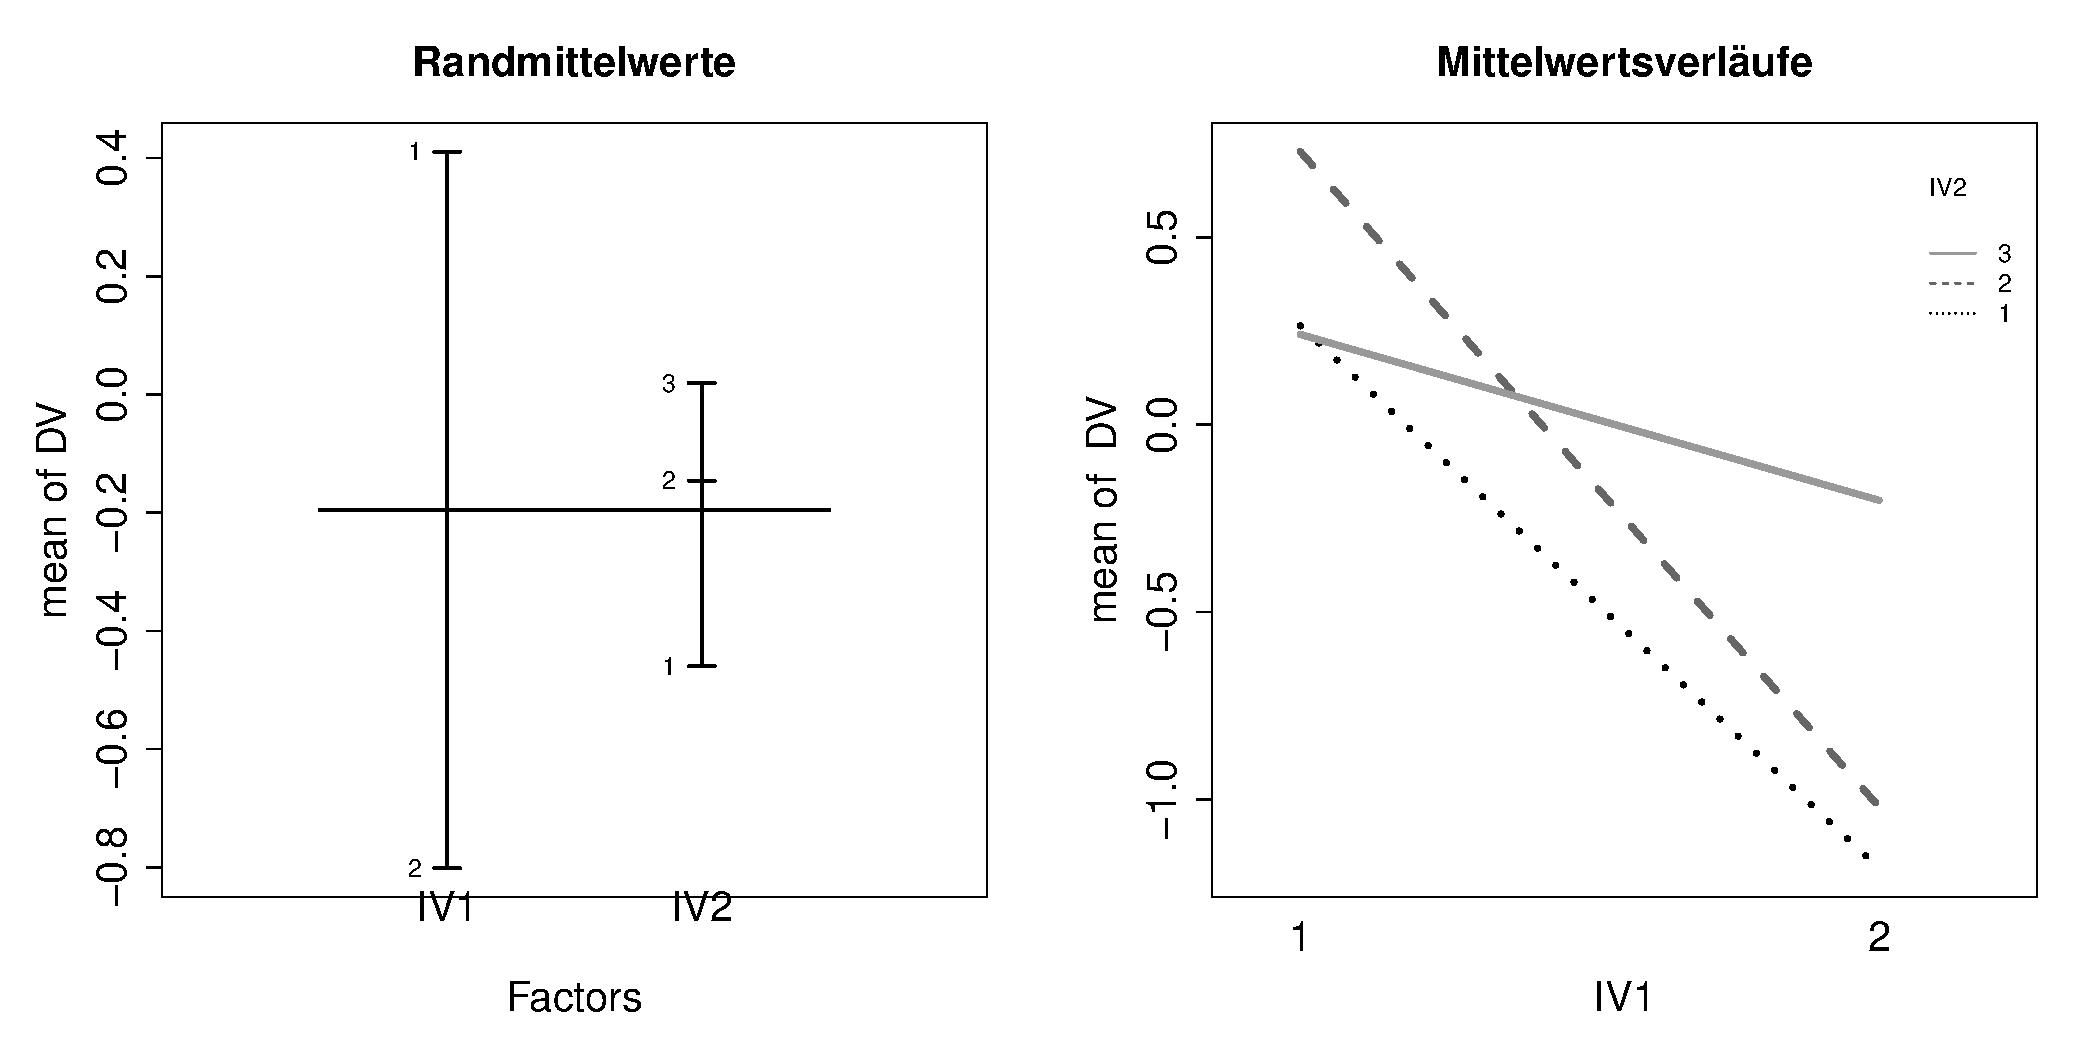
\includegraphics[width=12.5cm]{interactionPlot}
\vspace*{-0.5em}
\caption{Darstellung der Randmittelwerte durch \lstinline!plot.design()! sowie der Gruppenmittelwerte durch \lstinline!interaction.plot()!}
\label{fig:interactionPlot}
\end{figure}

%%%%%%%%%%%%%%%%%%%%%%%%%%%%%%%%%%%%%%%%%%%%%%%%%%%%%%%%%%%%%%%%%%
%%%%%%%%%%%%%%%%%%%%%%%%%%%%%%%%%%%%%%%%%%%%%%%%%%%%%%%%%%%%%%%%%%
\subsubsection{Effektstärke schätzen}
%%%%%%%%%%%%%%%%%%%%%%%%%%%%%%%%%%%%%%%%%%%%%%%%%%%%%%%%%%%%%%%%%%
%%%%%%%%%%%%%%%%%%%%%%%%%%%%%%%%%%%%%%%%%%%%%%%%%%%%%%%%%%%%%%%%%%

\index{Varianzanalyse!Effektstärke}
\index{etaSq@$\hat{\eta}^{2}$ (Effektstärke)}
Als Maß für die Stärke jedes getesteten Effekts kann das partielle $\eta_{p}^{2}$ herangezogen werden, zu dessen Schätzung $\hat{\eta}_{p}^{2}$ jeweils seine Effekt-Quadratsumme an der Summe von ihr und der Residual-Quadratsumme relativiert wird. Die Berechnung -- inkl.\ des einfachen $\hat{\eta}^{2}$ -- übernimmt\index[func]{EtaSq()@\lstinline{EtaSq()}} \lstinline!EtaSq(<<aov-Objekt>>)! aus dem Paket\index[pack]{DescTools@\lstinline{DescTools}} \lstinline!DescTools!.
\begin{lstlisting}
> library(DescTools)                         # für EtaSq()
> EtaSq(aovCRFpq, type=1)
             eta.sq  eta.sq.part
IV1      0.23816098   0.25778017
IV2      0.02561867   0.03601418
IV1:IV2  0.05048956   0.06857941

# Kontrolle
> anRes <- anova(lm(DV ~ IV1*IV2, data=dfCRFpq))
> SS1   <- anRes["IV1",       "Sum Sq"]      # Quadratsumme UV1
> SS2   <- anRes["IV2",       "Sum Sq"]      # Quadratsumme UV2
> SSI   <- anRes["IV1:IV2",   "Sum Sq"]      # Quadratsumme Interaktion
> SSE   <- anRes["Residuals", "Sum Sq"]      # Quadratsumme Residuen

> (etaSq1 <- SS1 / (SS1 + SS2 + SSI + SSE))  # eta^2 UV1
[1] 0.238161

> (etaSq2 <- SS2 / (SS1 + SS2 + SSI + SSE))  # eta^2 UV2
[1] 0.02561867

> (etaSqI <- SSI / (SS1 + SS2 + SSI + SSE))  # eta^2 Interaktion
[1] 0.05048956

> (pEtaSq1 <- SS1 / (SS1 + SSE))             # partielles eta^2 UV1
[1] 0.2577802

> (pEtaSq2 <- SS2 / (SS2 + SSE))             # partielles eta^2 UV2
[1] 0.03601418

> (pEtaSqI <- SSI / (SSI + SSE))             # part. eta^2 Interaktion
[1] 0.06857941
\end{lstlisting}

%%%%%%%%%%%%%%%%%%%%%%%%%%%%%%%%%%%%%%%%%%%%%%%%%%%%%%%%%%%%%%%%%%
%%%%%%%%%%%%%%%%%%%%%%%%%%%%%%%%%%%%%%%%%%%%%%%%%%%%%%%%%%%%%%%%%%
\subsection{Quadratsummen vom Typ I, II und III}
\label{sec:ssTypes}
%%%%%%%%%%%%%%%%%%%%%%%%%%%%%%%%%%%%%%%%%%%%%%%%%%%%%%%%%%%%%%%%%%
%%%%%%%%%%%%%%%%%%%%%%%%%%%%%%%%%%%%%%%%%%%%%%%%%%%%%%%%%%%%%%%%%%

\index{Varianzanalyse!Quadratsummen-Typen|textbf}
\index{Varianzanalyse!orthogonales Design}
In mehrfaktoriellen Designs mit unbalancierten Zellbesetzungen offenbart sich, dass R eine andere Methode zur Berechnung der Quadratsummen der Haupteffekte heranzieht, als es der Voreinstellung etwa von SAS, Stata oder SPSS entspricht.\footnote{Die hier verwendete Terminologie von \emph{Typen von Quadratsummen} wurde ursprünglich mit dem Programm SAS eingeführt und bezeichnet letztlich unterschiedliche Hypothesen in varianzanalytischen Designs mit mehreren Faktoren.} Für eine ausführlichere Darstellung s.\ Abschn.\ \ref{sec:multALManova}, \ref{sec:multALMmodCmp} sowie \citeA{Maxwell2004}.

R berechnet sequentielle Quadratsummen vom Typ I, für die bei unbalancierten Zellbesetzungen die Reihenfolge der im Modell berücksichtigten Terme bedeutsam ist. Die Quadratsumme eines Effekts wird hier als Reduktion der Quadratsumme der Residuen (\emph{residual sum of squares}, RSS) beim Wechsel zwischen den folgenden beiden Modellen berechnet: dem Modell mit allen Vorhersagetermen, die in der Modellformel vor dem zu testenden Effekt auftauchen und dem Modell, in dem zusätzlich dieser Effekt selbst berücksichtigt wird (Abschn.\ \ref{sec:regrCmp}). Der resultierende Test ist bei Haupteffekten äquivalent zur Frage, ob die zugehörigen gewichteten Randerwartungswerte identisch sind, wobei die Gewichtung der Zellerwartungswerte bei ihrer Mittelung mit den Zellbesetzungen erfolgt. Die Summe aller Effekt-Quadratsummen ist hier gleich der RSS-Differenz vom vollständigen Modell und jenem, in dem kein Effekt, also nur der Gesamterwartungswert eingeht (\lstinline!<<AV>> ~ 1!).

Quadratsummen vom Typ II für Haupteffekte berechnen sich als RSS-Differenz beim Wechsel zwischen den zwei folgenden Modellen: dem Modell mit allen Haupteffekten, aber ohne deren Interaktion sowie demselben Modell ohne den jeweils interessierenden Haupteffekt (egal wo er in der Modellformel steht). Die Reihenfolge der Effekte im Modell ist dabei irrelevant. Für den Test der Interaktion wird das vollständige Modell (beide Haupteffekte und Interaktion) mit dem Modell verglichen, das nur beide Haupteffekte berücksichtigt.

SAS und SPSS dagegen verwenden in der Voreinstellung partielle Quadratsummen vom Typ III\@. Die Quadratsumme eines Effekts wird hier als RSS-Reduktion beim Wechsel zwischen zwei anderen Modellen berechnet: dem Modell mit allen Vorhersagetermen außer dem interessierenden Effekt (egal ob vor oder nach diesem in der Modellformel stehend) und dem vollständigen Modell mit allen Termen. Die Reihenfolge der Effekte im Modell ist dabei irrelevant. Die Summe aller einzelnen Effekt-Quadratsummen hat hier bei unbalancierten Zellbesetzungen keine Bedeutung. Der so berechnete Test ist bei Haupteffekten äquivalent zur Frage, ob die gleichgewichteten Randerwartungswerte übereinstimmen.\footnote{\label{ftn:ssTypesCodes}Die genannte Äquivalenz von Modellvergleichen und Hypothesen über ungewichtete Randerwartungswerte setzt voraus, dass ein passendes Codierschema für kategoriale Variablen verwendet wird, z.\,B.\ die Effektcodierung (\citeNP{Venables2016}; Abschn.\ \ref{sec:multALManova}).}

Unabhängig vom Quadratsummen-Typ ist die Fehler-Quadratsumme beim Test einer Hypothese immer jene des vollständigen Modells mit allen Vorhersagetermen der Modellformel. Es handelt sich bei Quadratsummen vom Typ I, II und III letztlich nicht um verschiedene Berechnungsmethoden desselben Kennwertes, stattdessen dienen sie Tests inhaltlich unterschiedlicher Fragestellungen, die sich bei Haupteffekten auf unterschiedliche Modellvergleiche beziehen. Der Test der Interaktion stimmt hingegen bei allen Typen überein. Bei proportional ungleichen Zellbesetzungen\footnote{Proportional ungleiche Zellbesetzungen liegen vor, wenn $\frac{n_{jk}}{n_{jk'}} = \frac{n_{j'k}}{n_{j'k'}}$ sowie $\frac{n_{jk}}{n_{j'k}} = \frac{n_{jk'}}{n_{j'k'}}$ für alle $j, j', k, k'$ gilt.} ist zudem der Test der Haupteffekte beim Typ I gleich jenem beim Typ II. Im Spezialfall gleicher Zellbesetzungen liefern die Quadratsummen vom Typ I, II und III dieselben Ergebnisse.

Das folgende Beispiel eines CRF-$33$ Designs mit unbalancierten Zellbesetzungen ist jenes aus \citeA[p.~375]{Maxwell2004}. Zunächst folgen die Modellvergleiche, die zu Quadratsummen vom Typ I führen, daraufhin die Berechnung der Quadratsummen vom Typ III\@.
\begin{lstlisting}
> mdP <- 3                                    # Anzahl Stufen UV1
> mdQ <- 3                                    # Anzahl Stufen UV2

# AV Daten aus Bedingungen 1-1, 1-2, 1-3, 2-1, 2-2, 2-3, 3-1, 3-2, 3-3
> g11  <- c(41, 43, 50)
> g12  <- c(51, 43, 53, 54, 46)
> g13  <- c(45, 55, 56, 60, 58, 62, 62)
> g21  <- c(56, 47, 45, 46, 49)
> g22  <- c(58, 54, 49, 61, 52, 62)
> g23  <- c(59, 55, 68, 63)
> g31  <- c(43, 56, 48, 46, 47)
> g32  <- c(59, 46, 58, 54)
> g33  <- c(55, 69, 63, 56, 62, 67)
> mdDV <- c(g11, g12, g13, g21, g22, g23, g31, g32, g33) # Gesamt-Daten

# Zugehörige Faktoren UV1, UV2, Datensatz
> mdIV1 <- factor(rep(1:mdP, c(3+5+7, 5+6+4, 5+4+6)))
> mdIV2 <- factor(rep(rep(1:mdQ, mdP), c(3,5,7, 5,6,4, 5,4,6)))
> dfMD  <- data.frame(IV1=mdIV1, IV2=mdIV2, DV=mdDV)

# Quadratsummen vom Typ I aus anova()
> anova(lm(DV ~ IV1 + IV2 + IV1:IV2, data=dfMD))
Analysis of Variance Table
Response: DV
           Df   Sum Sq  Mean Sq  F value     Pr(>F)
IV1         2   101.11    50.56   1.8102     0.1782
IV2         2  1253.19   626.59  22.4357  4.711e-07 ***
IV1:IV2     4    14.19     3.55   0.1270     0.9717
Residuals  36  1005.42    27.93

# manuelle Berechnung der Quadratsummen vom Typ I aus dem
# Vergleich der sequentiell aufeinander aufbauenden Modelle
> SSI1 <- anova(lm(DV ~ 1,       dfMD), lm(DV ~ IV1,             dfMD))
> SSI2 <- anova(lm(DV ~ IV1,     dfMD), lm(DV ~ IV1+IV2,         dfMD))
> SSIi <- anova(lm(DV ~ IV1+IV2, dfMD), lm(DV ~ IV1+IV2+IV1:IV2, dfMD))

> SSI1[2, "Sum of Sq"]                          # QS Typ I von UV1
[1] 101.1111

> SSI2[2, "Sum of Sq"]                          # QS Typ I von UV2
[1] 1253.189

> SSIi[2, "Sum of Sq"]                          # QS der Interaktion
[1] 14.18714

# Vergleich des Gesamtmodells mit jenem ohne Effekte
> SSIt <- anova(lm(DV ~ 1, dfMD), lm(DV ~ IV1 + IV2 + IV1:IV2, dfMD))
> SSIt[2, "Sum of Sq"]                          # QS Gesamtmodell
[1] 1368.487

# Summe aller einzelnen Quadratsummen vom Typ I
> SSI1[2, "Sum of Sq"] + SSI2[2, "Sum of Sq"] + SSIi[2, "Sum of Sq"]
[1] 1368.487
\end{lstlisting}

In R gibt es im wesentlichen zwei Möglichkeiten, Quadratsummen vom Typ III zu erhalten. Zum einen kann mit \lstinline!drop1()!\index[func]{drop1()@\lstinline{drop1()}} (Abschn.\ \ref{sec:regrCmp}) die RSS-Änderung berechnet werden, die sich jeweils ergibt, wenn ein Vorhersageterm aus der Modellformel gestrichen wird und alle anderen beibehalten werden. Diese Vergleiche liegen gerade Quadratsummen vom Typ III zugrunde. Die Quadratsumme der Residuen steht in der Ausgabe in der Zeile \lstinline!<none>!. Zum anderen testet \lstinline!Anova()!\index[func]{Anova()@\lstinline{Anova()}} aus dem Paket \lstinline!car! mit Quadratsummen vom Typ III, wenn das Argument \lstinline!type="III"! gesetzt ist (analog Quadratsummen vom Typ II, s.\ Abschn.\ \ref{sec:AnovaRBp}). In beiden Fällen ist das \lstinline!contrasts! Argument für \lstinline!lm()!\index[func]{lm()@\lstinline{lm()}} notwendig, um von der\index{Varianzanalyse!Dummy-Codierung} Dummy-Codierung (Treatment-Kontraste) zur Effektcodierung\index{Varianzanalyse!Effektcodierung} der UVn zu wechseln (Abschn.\ \ref{sec:multALManova}).
\begin{lstlisting}
# lineares Modell mit Effektcodierung
> fitIII <- lm(DV ~ IV1 + IV2 + IV1:IV2, data=dfMD,
+              contrasts=list(IV1=contr.sum, IV2=contr.sum))

> drop1(fitIII, ~ ., test="F")                # QS Typ III aus drop1()
Single term deletions
Model:
DV ~ IV1 + IV2 + IV1:IV2

         Df  Sum of Sq      RSS     AIC  F value     Pr(>F)
<none>                  1005.42  157.79
IV1       2     204.76  1210.19  162.13   3.6658    0.03556 *
IV2       2    1181.11  2186.53  188.75  21.1452  8.447e-07 ***
IV1:IV2   4      14.19  1019.61  150.42   0.1270    0.97170

> library(car)                                # für Anova()
> Anova(fitIII, type="III")                   # QS Typ III ...
\end{lstlisting}

Die Quadratsumme der Interaktion unterscheidet sich nicht zwischen Typ I, II und III, die hier alle dieselben Modellvergleiche verwenden: Das eingeschränkte Modell ist immer das mit beiden Haupteffekten, das vollständige bzw.\ sequentiell folgende Modell jenes mit beiden Haupteffekten und ihrer Interaktion. Es folgt die manuelle Berechnung der Quadratsummen vom Typ III der Haupteffekte.
\begin{lstlisting}
> (MjkMD <- tapply(mdDV, list(mdIV1, mdIV2), mean))   # Zellmittelwerte
          1      2         3
1  44.66667  49.40  56.85714
2  48.60000  56.00  61.25000
3  48.00000  54.25  62.00000

> (NjkMD <- table(mdIV1, mdIV2))              # Zellbesetzungen
   1  2  3
1  3  5  7
2  5  6  4
3  5  4  6

> Mj <- rowMeans(MjkMD)                       # ungewichtete Zeilen-M
> Mk <- colMeans(MjkMD)                       # ungewichtete Spalten-M

# effektive Rand-Ns aus harmonischem Mittel der Zellen-Ns
> effNj <- 1 / rowMeans(1/NjkMD)              # harm. Mittel Zeilen-N
> effNk <- 1 / colMeans(1/NjkMD)              # harm. Mittel Spalten-N

# Gesamtmittel aus gewichteten Zeilen-Ms, bzw. gewichteten Spalten-Ms
> gM1 <- sum(effNj*Mj) / sum(effNj)           # aus Zeilen-Ms
> gM2 <- sum(effNk*Mk) / sum(effNk)           # aus Spalten-Ms

# QS Typ III - mdP bzw. mdQ * quadrierte Differenzen der Randmittel
# zum zugehörigen Gesamtmittel, gewichtet mit dem effektiven Rand-N
> (SSIII1 <- mdP * sum(effNj * (Mj-gM1)^2))   # QS Typ III UV1
[1] 204.7617

> (SSIII2 <- mdQ * sum(effNk * (Mk-gM2)^2))   # QS Typ III UV2
[1] 1181.105

# QS Residuen - Summe der quadrierten Differenzen zum Zellenmittel
> (SSE <- sum((mdDV - ave(mdDV, mdIV1, mdIV2, FUN=mean))^2))
[1] 1005.424
\end{lstlisting}

Der $F$-Bruch eines Effekts ergibt sich als Quotient der Effekt-Quadratsumme dividiert durch ihre Freiheitsgrade und der Quadratsumme der Residuen des vollständigen Modells dividiert durch ihre Freiheitsgrade.
\begin{lstlisting}
> dfSS1  <- mdP - 1                          # Freiheitsgrade QS UV1
> dfSS2  <- mdQ - 1                          # Freiheitsgrade QS UV2
> dfSSE  <- sum(NjkMD - 1)  # Freiheitsgrade QS Residuen vollst. Modell
> (Fval1 <- (SSIII1/dfSS1) / (SSE/dfSSE))    # Teststatistik F-Wert UV1
[1] 3.665829

> (Fval2 <- (SSIII2/dfSS2) / (SSE/dfSSE))    # Teststatistik F-Wert UV2
[1] 21.14520

> (pVal1 <- pf(Fval1, dfSS1, dfSSE, lower.tail=FALSE))  # p-Wert UV1
[1] 0.03555901

> (pVal2 <- pf(Fval2, dfSS2, dfSSE, lower.tail=FALSE))  # p-Wert UV2
[1] 8.44678e-07
\end{lstlisting}

%%%%%%%%%%%%%%%%%%%%%%%%%%%%%%%%%%%%%%%%%%%%%%%%%%%%%%%%%%%%%%%%%%
%%%%%%%%%%%%%%%%%%%%%%%%%%%%%%%%%%%%%%%%%%%%%%%%%%%%%%%%%%%%%%%%%%
\subsection{Bedingte Haupteffekte testen}
\label{sec:simpleEffects}
%%%%%%%%%%%%%%%%%%%%%%%%%%%%%%%%%%%%%%%%%%%%%%%%%%%%%%%%%%%%%%%%%%
%%%%%%%%%%%%%%%%%%%%%%%%%%%%%%%%%%%%%%%%%%%%%%%%%%%%%%%%%%%%%%%%%%

Im Folgenden sei wieder das balancierte Design aus Abschn.\ \ref{sec:CRFpqAov} betrachtet.

\index{Varianzanalyse!bedingte Haupteffekte}
\index{Varianzanalyse!simple effects}
Dem Test der bedingten Haupteffekte (\emph{simple effects}) der ersten UV im CRF-$pq$ Design liegt folgende Frage zugrunde: Stimmen in einer festen Stufe $k$ der zweiten UV alle Zellerwartungswerte $\mu_{jk}$ mit $1 \leq j \leq p$ überein und sind damit gleich dem zugehörigen Randerwartungswert $\mu_{.k}$ (Tab.\ \ref{tab:CRF23})? Für jede der $q$ Stufen der zweiten UV lässt sich ein solcher bedingter Haupteffekt der ersten UV testen. Analog soll der Test eines bedingten Haupteffekts der zweiten UV in einer festen Stufe $j$ der ersten UV prüfen, ob alle Zellerwartungswerte $\mu_{jk}$ mit $1 \leq k \leq q$ übereinstimmen und damit gleich dem zugehörigen Randerwartungswert $\mu_{j.}$ sind. Für die zweite UV können $p$ bedingte Haupteffekte getestet werden.

%\begin{longtable}{rcccl}
\begin{table}[ht]
\centering
\caption{CRF-$23$ Designschema mit Zell- und Randerwartungswerten}
\label{tab:CRF23}
\begin{tabular}{rcccl}
\hline
~ & \sffamily UV2 -- 1 & \sffamily UV2 -- 2 & \sffamily UV2 -- 3 &
\sffamily Mittel\\\hline\hline
\sffamily UV1 -- 1 & $\mu_{11}$ & $\mu_{12}$ & $\mu_{13}$ & $\mu_{1.}$\\
\sffamily UV1 -- 2 & $\mu_{21}$ & $\mu_{22}$ & $\mu_{23}$ & $\mu_{2.}$\\
\sffamily Mittel   & $\mu_{.1}$ & $\mu_{.2}$ & $\mu_{.3}$ & $\mu$\\\hline
\end{tabular}
\end{table}
%\end{longtable}

Für den Test bedingter Haupteffekte stellt das Paket \lstinline!phia!\index[pack]{phia@\lstinline{phia}|textbf} \cite{DeRosarioMartinez2013} die Funktion\index[func]{testInteractions()@\lstinline{testInteractions()}} \lstinline!testInteractions()! bereit. Eine Alternative ist das Paket \lstinline!emmeans!\index[pack]{emmeans@\lstinline{emmeans}} (Abschn.\ \ref{sec:CRFpqAov}, Fußnote \ref{ftn:emmeans}).
\begin{lstlisting}
testInteractions(<<aov-Modell>>, fixed="<<Bedingung>>",
                 across="<<bedingte Haupteffekte>>",
                 adjustment="<<alpha-Adjustierung>>")
\end{lstlisting}

Zunächst ist ein mit \lstinline!aov()! angepasstes Modell zu übergeben. Für \lstinline!fixed! ist der Faktor mit den Stufen zu nennen, für die bedingte Haupteffekte des anderen Faktors berechnet werden sollen. Für den Test der bedingten Haupteffekte der UV1 auf allen Stufen der UV2 wäre also UV2 an \lstinline!fixed! zu übergeben. \lstinline!across! definiert den Faktor, für den bedingte Haupteffekte zu berechnen sind. Wie der Gefahr eines erhöhten Fehlers erster Art durch wiederholtes Testen zu begegnen ist, wird in der Literatur uneinheitlich beurteilt (für verschiedene Strategien vgl.\ \citeNP[p.~377~ff.]{Kirk1995}). Über \lstinline!adjustment! können unterschiedliche Methoden gewählt werden. \lstinline!testInteractions()! verfügt über viele weitere Testmöglichkeiten, die in der Hilfe erläutert sind.
\begin{lstlisting}
> library(phia)                               # für testInteractions()
> testInteractions(aovCRFpq, fixed="IV2", across="IV1",
+                  adjustment="none")
F Test:
P-value adjustment method: none
            Value Df Sum of Sq       F   Pr(>F)
1         1.44724  1     8.378  6.9243 0.011841 *
2         1.74857  1    12.230 10.1079 0.002772 **
3         0.44248  1     0.783  0.6472 0.425629
Residuals         42    50.818
\end{lstlisting}

Die Ergebnisse lassen sich manuell prüfen, hier am Beispiel des bedingten Haupteffekts der ersten UV in der ersten Stufe der zweiten UV. Dafür ist zum einen die einfaktorielle Varianzanalyse der ersten UV notwendig, durchgeführt für die erste Stufe der zweiten UV. Die Beschränkung der Daten auf die feste Stufe einer UV lässt sich mit dem \lstinline!subset! Argument von \lstinline!aov()! oder \lstinline!lm()! erreichen, dem ein geeigneter Indexvektor zu übergeben ist. Die mittlere Effekt-Quadratsumme dieser Varianzanalyse bildet den Zähler der $F$-Teststatistik. Wird die Voraussetzung der Varianzhomogenität als gegeben erachtet, ist der Nenner des $F$-Bruchs für alle Tests identisch und besteht aus der mittleren Quadratsumme der Residuen der zweifaktoriellen Varianzanalyse.
\begin{lstlisting}
# einfaktorielle ANOVAs für UV1 in 1. Stufe der UV2
> CRFp1 <- anova(lm(DV ~ IV1, data=dfCRFpq, subset=(IV2=="1")))

# extrahiere Effekt-Quadratsumme für bedingten Haupteffekt der UV1
> SSp1 <- CRFp1["IV1", "Sum Sq"]            # in Stufe 1 der UV2

# zweifaktorielle ANOVA: QS und df UV1, Interaktion, Residuen
> CRFpq <- anova(lm(DV ~ IV1*IV2, data=dfCRFpq))
> SSA   <- CRFpq["IV1",       "Sum Sq"]     # QS UV1
> SSE   <- CRFpq["Residuals", "Sum Sq"]     # QS Residuen
> dfSSA <- CRFpq["IV1",       "Df"]         # Freiheitsgrade QS UV1
> dfSSE <- CRFpq["Residuals", "Df"]         # Freiheitsgrade Fehler

# F-Wert des bedingten Haupteffekts der UV1
> Fp1  <- (SSp1/dfSSA) / (SSE/dfSSE)        # in Stufe 1 der UV2
> (pP1 <- pf(Fp1, dfSSA, dfSSE, lower.tail=FALSE))      # p-Wert
[1] 0.01184106
\end{lstlisting}

%%%%%%%%%%%%%%%%%%%%%%%%%%%%%%%%%%%%%%%%%%%%%%%%%%%%%%%%%%%%%%%%%%
%%%%%%%%%%%%%%%%%%%%%%%%%%%%%%%%%%%%%%%%%%%%%%%%%%%%%%%%%%%%%%%%%%
\subsection{Beliebige a-priori Kontraste}
\label{sec:contrCRFpq}
%%%%%%%%%%%%%%%%%%%%%%%%%%%%%%%%%%%%%%%%%%%%%%%%%%%%%%%%%%%%%%%%%%
%%%%%%%%%%%%%%%%%%%%%%%%%%%%%%%%%%%%%%%%%%%%%%%%%%%%%%%%%%%%%%%%%%

\index{Varianzanalyse!Kontraste!a-priori}
Im Vergleich zum einfaktoriellen Fall im CR-$p$ Design ergeben sich für beliebige a-priori Kontraste im CRF-$pq$ Design einige Änderungen, da es nun verschiedene Typen von Kontrasten gibt. Zunächst sind dies jene Kontraste, die sich auf die\index{Varianzanalyse!assoziierte einfaktorielle} \emph{assoziierte} einfaktorielle Varianzanalyse beziehen. Dies bedeutet, dass die faktorielle Struktur der Bedingungskombinationen ignoriert wird, stattdessen werden alle Bedingungskombinationen als Stufen einer einzigen (künstlichen) UV betrachtet. Aus einem Design mit zwei Stufen der ersten und drei Stufen der zweiten UV würde so eines mit $2 \cdot 3=6$ Stufen einer einzigen UV\@. Innerhalb dieser assoziierten einfaktoriellen Situation lassen sich nun Kontraste wie in Abschn.\ \ref{sec:contrCRp} formulieren und testen.

Die mittlere Quadratsumme der Residuen aus der zweifaktoriellen Varianzanalyse ist dieselbe wie die mittlere Quadratsumme innerhalb der Gruppen aus der assoziierten einfaktoriellen Varianzanalyse. Zu beachten ist die Reihenfolge der Stufen in der assoziierten einfaktoriellen Situation. Sie wird hier durch die Stufen des künstlichen Faktors bestimmt, dessen Ausprägung von der Kombination der Faktorstufen der beiden UVn abhängt.

Im Beispiel soll das bereits verwendete CRF-$23$ Design mit dem in Tab.\ \ref{tab:CRF23} dargestellten Schema vorliegen. Als assoziiertes einfaktorielles Schema ergibt sich das in Tab.\ \ref{tab:CRF23assoc} aufgeführte.

%\begin{longtable}{ccccccl}
\begin{table}[ht]
\centering
\caption{Assoziiertes einfaktorielles Schema zum CRF-$23$ Design}
\label{tab:CRF23assoc}
\begin{tabular}{ccccccl}
\hline
\sffamily UVcomb -- 1 & \sffamily UVcomb -- 2 & \sffamily UVcomb -- 3 & \sffamily UVcomb -- 4 & \sffamily UVcomb -- 5 & \sffamily UVcomb -- 6 & \sffamily M\\\hline\hline
$\mu_{11}$ & $\mu_{21}$ & $\mu_{12}$ & $\mu_{22}$ & $\mu_{13}$ & $\mu_{23}$ & $\mu$\\\hline
\end{tabular}
\end{table}
%\end{longtable}

\begin{lstlisting}
# assoziierte einfaktorielle sowie die zweifaktorielle ANOVA
> CRFpq1 <- anova(lm(DV ~ IVcomb,  data=dfCRFpq))
> CRFpq2 <- anova(lm(DV ~ IV1*IV2, data=dfCRFpq))

# prüfe MS within = MS error
> all.equal(CRFpq1["Residuals", "Mean Sq"],
+           CRFpq2["Residuals", "Mean Sq"])
[1] TRUE
\end{lstlisting}

Mit \lstinline!glht()!\index[func]{glht()@\lstinline{glht()}} aus dem Paket \lstinline!multcomp!\index[pack]{multcomp@\lstinline{multcomp}} soll im Beispiel das Mittel der Erwartungswerte $\mu_{11}$ und $\mu_{12}$ gegen das Mittel der verbleibenden vier Gruppenerwartungswerte getestet werden. Unter $\text{H}_{0}$ soll der Kontrast gleich $0$ sein, unter $\text{H}_{1}$ größer als $0$.
\begin{lstlisting}
> library(multcomp)                                    # für glht()
> aovComb <- aov(DV ~ IVcomb, data=dfCRFpq)            # aov-Modell

# Matrix der Kontrastkoeffizienten - hier nur eine Zeile
> cntrMat <- rbind("contr 01"=c(1/2, -1/4, 1/2, -1/4, -1/4, -1/4))
> summary(glht(aovComb, linfct=mcp(IVcomb=cntrMat),
+              alternative="greater"))
Simultaneous Tests for General Linear Hypotheses
Multiple Comparisons of Means: User-defined Contrasts
Fit: aov(formula = DV ~ IVcomb, data = dfCRFpq)
Linear Hypotheses:
               Estimate  Std. Error  t value   Pr(>t)
contr 01 <= 0    1.0372      0.3368     3.08  0.00182 **
\end{lstlisting}

Da die Gruppengrößen hier gleich sind, vereinfacht sich die Formel für die Teststatistik in der manuellen Berechnung, da nicht mehr gruppenweise mit der Anzahl der Beobachtungen gewichtet werden muss.
\begin{lstlisting}
> Mjk     <- tapply(DV, IVcomb, mean)                # Zellenmittel
> dfSSE   <- (Njk-1)*P*Q                             # df von QS error
> SSE     <- sum((DV - ave(DV, IVcomb, FUN=mean))^2) # QS error
> MSE     <- SSE / dfSSE                             # MS error
> (psiHat <- sum(cntrMat[1, ] * Mjk))                # Kontrastschätzer
[1] 1.03724

> lenSq  <- sum(cntrMat[1, ]^2  / Njk)               # quadrierte Länge
> (tStat <- psiHat / sqrt(lenSq*MSE))                # Teststatistik t
[1] 3.079714

> (tCrit <- qt(0.05, dfSSE, lower.tail=FALSE)) # krit. t-Wert einseitig
[1] 1.681952

> (pVal <- pt(abs(tStat), dfSSE, lower.tail=FALSE))  # p-Wert einseitig
[1] 0.001822898

# untere Grenze des einseitigen 95%-Vertrauensintervalls für psi
> (ciLo <- psiHat - tCrit*sqrt(lenSq*MSE))
[1] 0.4707625
\end{lstlisting}

Sollen mehrere Kontraste gleichzeitig getestet werden, ist dies durch Zusammenstellung der zugehörigen Kontrastvektoren als (ggf.\ benannte) Zeilen einer Matrix möglich. Hier werden drei Kontraste ohne Adjustierung des $\alpha$-Niveaus getestet.
\begin{lstlisting}
# Matrix der Kontrastkoeffizienten
> cntrMat <- rbind("contr 01"=c( 1/2, -1/4, 1/2, -1/4, -1/4, -1/4),
+                  "contr 02"=c(   0,    0,   1,    0,   -1,    0),
+                  "contr 03"=c(-1/2, -1/2, 1/4,  1/4,  1/4,  1/4))

> library(multcomp)                             # für glht()
> (sumRes <- summary(glht(aovComb, linfct=mcp(IVcomb=cntrMat),
+                         alternative="greater"),
+                    test=adjusted("none")))
Simultaneous Tests for General Linear Hypotheses
Multiple Comparisons of Means: User-defined Contrasts
Fit: aov(formula = DV ~ IVcomb, data = dfCRFpq)
Linear Hypotheses:
               Estimate  Std. Error  t value   Pr(>t)
contr 01 <= 0    1.0372      0.3368    3.080  0.00182 **
contr 02 <= 0    0.4878      0.5500    0.887  0.19009
contr 03 <= 0    0.3969      0.3368    1.178  0.12264

# manuelle Berechnung
> psiHats <- cntrMat   %*% Mjk                # Kontrastschätzungen
> lenSqs  <- cntrMat^2 %*% (1/rep(Njk, ncol(cntrMat)))  # quadr. Längen
> tStats  <- psiHats / sqrt(lenSqs*MSE)       # Teststatistiken
> pVals   <- pt(abs(tStats), dfSSE, lower.tail=FALSE)   # p-Werte eins.
> data.frame(psiHats, tStats, pVals)
            psiHats     tStats        pVals
contr 01  1.0372399  3.0797137  0.001822898
contr 02  0.4877878  0.8869062  0.190090003
contr 03  0.3968684  1.1783590  0.122643406
\end{lstlisting}

Neben allgemeinen Kontrasten, die sich auf das assoziierte einfaktorielle Design beziehen, gibt es in der zweifaktoriellen Situation drei weitere Kontrasttypen, auch \emph{Familien} von Kontrasten genannt: Linearkombinationen der mittleren Erwartungswerte in den Stufen der ersten UV (\emph{$A$-Kontraste}), solche der mittleren Erwartungswerte in den Stufen der zweiten UV (\emph{$B$-Kontraste}) und Interaktions-Kontraste (\emph{$I$-Kontraste}). Alle drei zeichnen sich dadurch aus, dass sich die Koeffizienten der Linearkombination nicht nur insgesamt zu $0$ summieren, sondern zudem weitere Nebenbedingungen erfüllen, wenn sie in das Designschema eingetragen werden:

\begin{itemize}
\item $A$-Kontraste werden mit Koeffizienten gebildet, die im Designschema in jeder Zeile konstant sind und sich pro Spalte zu $0$ summieren. Im obigen Beispiel mit der entsprechenden Reihenfolge der Zellen würde etwa der Kontrast $(\frac{1}{3}, -\frac{1}{3}, \frac{1}{3}, -\frac{1}{3}, \frac{1}{3}, -\frac{1}{3})$ den mittleren Erwartungswert $\mu_{1.}$ gegen den mittleren Erwartungswert $\mu_{2.}$ testen.
\item $B$-Kontraste werden mit Koeffizienten gebildet, die im Designschema in jeder Spalte konstant sind und sich pro Zeile zu $0$ summieren. Im obigen Beispiel mit der entsprechenden Reihenfolge der Zellen würde etwa der Kontrast $(\frac{1}{2}, \frac{1}{2}, -\frac{1}{4}, -\frac{1}{4}, -\frac{1}{4}, -\frac{1}{4})$ den mittleren Erwartungswert $\mu_{.1}$ gegen das Mittel der mittleren Erwartungswerte $\mu_{.2}$ und $\mu_{.3}$ testen.
\item $I$-Kontraste werden mit Koeffizienten gebildet, die sich im Designschema sowohl pro Zeile als auch pro Spalte zu $0$ summieren. Im obigen Beispiel mit der entsprechenden Reihenfolge der Zellen würde etwa der Kontrast $(\frac{1}{2}, -\frac{1}{2}, -\frac{1}{4}, \frac{1}{4}, -\frac{1}{4}, \frac{1}{4})$ die Differenz der Gruppenerwartungswerte $\mu_{11}-\mu_{21}$ gegen das Mittel der beiden Differenzen der Gruppenerwartungswerte $\mu_{12}-\mu_{22}$ und $\mu_{13}-\mu_{23}$ testen.
\end{itemize}

$A$-, $B$- und $I$-Kontraste können genauso innerhalb der assoziierten einfaktoriellen Varianzanalyse\index{Varianzanalyse!assoziierte einfaktorielle} getestet werden wie allgemeine Kontraste. Statt mit den Gruppenerwartungswerten können $A$- und $B$-Kontraste zudem auch mit den mittleren Erwartungswerten formuliert werden. In diesem Fall ist die Teststatistik entsprechend anders zu bilden, der kritische Wert ändert sich dagegen nicht.

Im Beispiel sollen die oben genannten $A$- und $B$-Kontraste mit Hilfe der mittleren Erwartungswerte formuliert werden.
\begin{lstlisting}
# A-Kontrast aus Randmittelwerten der UV1
> meansA   <- tapply(dfCRFpq$DV, dfCRFpq$IV1, mean) # Zeilenmittel
> cntrVecA <- c(1, -1)                              # Kontrastvektor
> psiHatA  <- sum(cntrVecA * meansA)                # Kontrastschätzung
> lenSqA   <- sum(cntrVecA^2 / (Q*Njk))             # quadrierte Länge
> (statA   <- psiHatA / sqrt(lenSqA*MSE))           # Teststatistik
[1] 3.819294

# B-Kontrast aus Randmittelwerten der UV2
> meansB   <- tapply(dfCRFpq$DV, dfCRFpq$IV2, mean) # Spaltenmittel
> cntrVecB <- c(1, -1/2, -1/2)                      # Kontrastvektor
> psiHatB  <- sum(cntrVecB * meansB)                # Kontrastschätzung
> lenSqB   <- sum(cntrVecB^2 / (P*Njk))             # quadrierte Länge
> (statB   <- psiHatB / sqrt(lenSqB*MSE))           # Teststatistik
[1] -1.178359
\end{lstlisting}

%%%%%%%%%%%%%%%%%%%%%%%%%%%%%%%%%%%%%%%%%%%%%%%%%%%%%%%%%%%%%%%%%%
%%%%%%%%%%%%%%%%%%%%%%%%%%%%%%%%%%%%%%%%%%%%%%%%%%%%%%%%%%%%%%%%%%
\subsection{Beliebige post-hoc Kontraste nach Scheffé}
%%%%%%%%%%%%%%%%%%%%%%%%%%%%%%%%%%%%%%%%%%%%%%%%%%%%%%%%%%%%%%%%%%
%%%%%%%%%%%%%%%%%%%%%%%%%%%%%%%%%%%%%%%%%%%%%%%%%%%%%%%%%%%%%%%%%%

\index{Varianzanalyse!Kontraste!zweifaktoriell}
\index{Varianzanalyse!Kontraste!post-hoc (Scheffé)}
Beliebige Kontraste können auch im Anschluss an eine signifikante Varianzanalyse getestet werden. Die zweifaktorielle Varianzanalyse prüft beim Test der Effekte (zwei Haupteffekte, ein Interaktionseffekt) implizit simultan alle möglichen zugehörigen Kontraste ($A$, $B$ oder $I$) -- spezifische Hypothesen liegen also bei ihrer Anwendung nicht vor. Aus diesem Grund muss im Anschluss an eine Varianzanalyse bei Einzeltests eine geeignete\index{alpha-Adjustierung@$\alpha$-Adjustierung} $\alpha$-Adjustierung vorgenommen werden, hier vorgestellt nach der Methode von Scheffé.\footnote{Für weitere vgl.\ \lstinline!?PostHocTest!\index[func]{PostHocTest()@\lstinline{PostHocTest()}} aus dem Paket\index[pack]{DescTools@\lstinline{DescTools}} \lstinline!DescTools!.} Sie ist in\index[func]{ScheffeTest()@\lstinline{ScheffeTest()}} \lstinline!ScheffeTest()! aus dem Paket\index[pack]{DescTools@\lstinline{DescTools}} \lstinline!DescTools! implementiert (Abschn.\ \ref{sec:contrCRp}).

Hier soll wieder das Mittel der Erwartungswerte $\mu_{11}$ und $\mu_{12}$ gegen das Mittel der verbleibenden vier Gruppenerwartungswerte gerichtet getestet werden. Da es sich hierbei nicht um einen $A$, $B$ oder $I$-Kontrast handelt, soll in der assoziierten einfaktoriellen Situation getestet werden, was zu einer sehr konservativen $\alpha$-Adjustierung führt.
\begin{lstlisting}
# transponiere cntrMat mit t(), damit Koeffizienten in Spalte stehen
> aovComb <- aov(DV~IVcomb, data=dfCRFpq)   # assoziierte 1-fakt. ANOVA
> library(DescTools)                        # für ScheffeTest()
> ScheffeTest(aovComb, which="IVcomb", contrasts=t(cntrMat))
Posthoc multiple comparisons of means : Scheffe Test
95% family-wise confidence level
Fit: aov(formula = DV ~ IVcomb, data = dfCRFpq)
$IVcomb
                              diff      lwr.ci    upr.ci    pval
1.1,1.2-2.1,2.2,1.3,2.3  1.0372399  -0.1385869  2.213067  0.1153
1.2-1.3                  0.4877878  -1.4323293  2.407905  0.9766
1.2,2.2,1.3,2.3-1.1,2.1  0.3968684  -0.7789584  1.572695  0.9228
\end{lstlisting}

Für die manuelle Kontrolle gilt zunächst alles bereits für beliebige a-priori Kontraste Ausgeführte. Lediglich die Wahl des kritischen Wertes weicht ab und ergibt sich zur $\alpha$-Adjustierung aus einer $F$-Verteilung. Dieser kritische Wert ist mit dem Quadrat der a-priori $t$-Teststatistik zu vergleichen -- die etwa in der von \lstinline!summary(glht(...))! zurückgegebenen Liste in der Komponente \lstinline!test$tstat! steht.
\begin{lstlisting}
> (Fstat <- sumRes$test$tstat^2)             # quadrierte Teststatistik
 contr 01   contr 02   contr 03
9.4846366  0.7866025  1.3885299

# df von SS between aus der assoziierten einfaktoriellen Varianzanalyse
> dfSSba <- P*Q - 1

# kritischer F-Wert für quadrierte Teststatistik
> (Fcrit <- dfSSba * qf(0.05, df1=dfSSba, df2=dfSSE, lower.tail=FALSE))
[1] 12.18846

# p-Wert einseitig
> (pVal <- pf(Fstat/dfSSba, dfSSba, dfSSE, lower.tail=FALSE))
 contr 01   contr 02   contr 03
0.1152858  0.9766012  0.9227677
\end{lstlisting}

Die Wahl des kritischen Wertes erfolgte hier so, dass alle möglichen Kontraste aus der assoziierten einfaktoriellen Varianzanalyse zugelassen sind. Sollen die Kontraste dagegen nur aus einem Unterraum des Kontrastraumes stammen, etwa weil jeweils nur Kontraste aus einer Familie ($A$, $B$ oder $I$) von Interesse sind, kann der kritische $F$-Wert wie folgt gewählt werden. In diesem Fall erfolgt eine gleichzeitige\index{alpha-Adjustierung@$\alpha$-Adjustierung} $\alpha$-Adjustierung nur für Kontraste aus der gewählten Familie, woraus ein geringerer kritischer Wert resultiert:
\begin{itemize}
\item $A$-Kontraste ($p$ Stufen): \lstinline!(P-1) * qf(1-0.05, P-1, dfSSE))!
\item $B$-Kontraste ($q$ Stufen): \lstinline!(Q-1) * qf(1-0.05, Q-1, dfSSE))!
\item $I$-Kontraste: \lstinline!(P-1) * (Q-1) * qf(1-0.05, (P-1)*(Q-1), dfSSE))!
\end{itemize}

%%%%%%%%%%%%%%%%%%%%%%%%%%%%%%%%%%%%%%%%%%%%%%%%%%%%%%%%%%%%%%%%%%
%%%%%%%%%%%%%%%%%%%%%%%%%%%%%%%%%%%%%%%%%%%%%%%%%%%%%%%%%%%%%%%%%%
\subsection{Marginale Paarvergleiche nach Tukey}
%%%%%%%%%%%%%%%%%%%%%%%%%%%%%%%%%%%%%%%%%%%%%%%%%%%%%%%%%%%%%%%%%%
%%%%%%%%%%%%%%%%%%%%%%%%%%%%%%%%%%%%%%%%%%%%%%%%%%%%%%%%%%%%%%%%%%

\index{Varianzanalyse!Kontraste!Tukey HSD}
\index[func]{TukeyHSD()@\lstinline{TukeyHSD()}}
Alternativ zu beliebigen Kontrasten können im Anschluss an eine Varianzanalyse auch die Randerwartungswerte jeweils eines Faktors mit Tukey-Kontrasten paarweise miteinander verglichen werden (Abschn.\ \ref{sec:tukey}). Dafür ist in \lstinline!TukeyHSD()! für das Argument \lstinline!which! der Faktor zu nennen, dessen Stufen verglichen werden sollen. Die so durchgeführten Tests ignorieren allerdings eine ggf.\ im Modell vorhandene Interaktion.
\begin{lstlisting}
> aovCRF <- aov(DV ~ IV1+IV2, data=dfCRFpq)   # Modell ohne Interaktion
> TukeyHSD(aovCRF, which="IV2")
Tukey multiple comparisons of means
95% family-wise confidence level
Fit: aov(formula = DV ~ IV1 + IV2, data = dfCRFpq)
$IV2
         diff        lwr      upr     p adj
2-1 0.3142383 -0.6406700 1.269147 0.7061067
3-1 0.4794984 -0.4754099 1.434407 0.4490851
3-2 0.1652602 -0.7896482 1.120168 0.9076526
\end{lstlisting}

Auch mit \lstinline!glht()! aus dem Paket \lstinline!multcomp! können Tukey Paarvergleiche der Randerwartungswerte getestet werden (Abschn.\ \ref{sec:tukey}).
\begin{lstlisting}
> library(multcomp)                               # für glht()
> tukey <- glht(aovCRF, linfct=mcp(IV2="Tukey"))  # Tukey Kontraste
> summary(tukey)                                  # Tests ...
> confint(tukey)                                  # Konfidenzintervalle
\end{lstlisting}

%%%%%%%%%%%%%%%%%%%%%%%%%%%%%%%%%%%%%%%%%%%%%%%%%%%%%%%%%%%%%%%%%%
%%%%%%%%%%%%%%%%%%%%%%%%%%%%%%%%%%%%%%%%%%%%%%%%%%%%%%%%%%%%%%%%%%
\section[Zweifaktorielle Varianzanalyse mit zwei Intra-Gruppen Faktoren (RBF-\texorpdfstring{$pq$}{pq})]{Zweifaktorielle Varianzanalyse mit zwei Intra-Gruppen Faktoren (RBF-$\bm{pq}$)}
\label{sec:RBFpq}
%%%%%%%%%%%%%%%%%%%%%%%%%%%%%%%%%%%%%%%%%%%%%%%%%%%%%%%%%%%%%%%%%%
%%%%%%%%%%%%%%%%%%%%%%%%%%%%%%%%%%%%%%%%%%%%%%%%%%%%%%%%%%%%%%%%%%

\index{Varianzanalyse!zweifaktorielle!abhängige Gruppen (RBF-$pq$)}
Liefert jede Person in jeder der von zwei Faktoren (UVn) gebildeten Bedingungskombinationen Beobachtungen einer Zielgröße (AV), spricht man von einem RBF-$pq$ Design (\emph{randomized block factorial}) mit $p$ Stufen der ersten und $q$ Stufen der zweiten UV\@. Die Reihenfolge, in der die $p \cdot q$ Bedingungen durchlaufen werden, ist für jede Person zu randomisieren. Ein Block aus $p \cdot q$ voneinander abhängigen Beobachtungen (eine aus jeder Bedingung) kann dabei auch von unterschiedlichen, z.\,B.\ bzgl.\ relevanter Störvariablen gematchten Personen stammen. Hierbei ist innerhalb eines Blocks die Zuteilung von Personen zu Bedingungen zu randomisieren.

Im Vergleich zum CRF-$pq$ Design wirkt im Modell zum RBF-$pq$ Design ein systematischer Effekt mehr am Zustandekommen einer Beobachtung mit: Zusätzlich zu den drei festen Effekten, die auf die Gruppenzugehörigkeit bzgl.\ der beiden UVn zurückgehen (beide Haupteffekte und der Interaktionseffekt), ist dies der zufällige\index{Varianzanalyse!Blockeffekt} Blockeffekt.

%%%%%%%%%%%%%%%%%%%%%%%%%%%%%%%%%%%%%%%%%%%%%%%%%%%%%%%%%%%%%%%%%%
%%%%%%%%%%%%%%%%%%%%%%%%%%%%%%%%%%%%%%%%%%%%%%%%%%%%%%%%%%%%%%%%%%
\subsection{Univariat formuliert auswerten und Effektstärke schätzen}
%%%%%%%%%%%%%%%%%%%%%%%%%%%%%%%%%%%%%%%%%%%%%%%%%%%%%%%%%%%%%%%%%%
%%%%%%%%%%%%%%%%%%%%%%%%%%%%%%%%%%%%%%%%%%%%%%%%%%%%%%%%%%%%%%%%%%

Wie im RB-$p$ Design (Abschn.\ \ref{sec:RBp}) müssen die Daten im\index{Datensatz!Long-Format} Long-Format (Abschn.\ \ref{sec:reshape}) inkl.\ eines Blockbildungsfaktors \lstinline!<<Block>>! der Klasse \lstinline!factor! vorliegen. Nicht alle möglichen Blöcke sind auch experimentell realisiert, sondern nur eine Zufallsauswahl -- \lstinline!<<Block>>! ist also ein\index{Varianzanalyse!Random-Faktor} Random-Faktor. In der Modellformel muss explizit angegeben werden, aus welchen additiven Komponenten sich die Quadratsumme innerhalb der Zellen zusammensetzt. Im RBF-$pq$ Design drückt\index[func]{Error()@\lstinline{Error()}} \lstinline!Error(<<Block>>/(<<UV1>>*<<UV2>>))! aus, dass \lstinline!<<Block>>! in den durch die Kombination von \lstinline!<<UV1>>! und \lstinline!<<UV2>>! entstehenden Bedingungen verschachtelt ist: Die durch die kombinierte Variation von UV1 und UV2 entstehenden Effekte in der AV (beide Haupteffekte und der Interaktionseffekt) sind daher jeweils innerhalb der durch \lstinline!<<Block>>! definierten Blöcke zu\index[func]{aov()@\lstinline{aov()}} analysieren.\footnote{Der Term lautet \lstinline!Error(<<Block>> + <<Block>>:<<UV1>> + <<Block>>:<<UV2>> + <<Block>>:<<UV1>>:<<UV2>>)!, wenn er ausgeschrieben wird. Dies sind die vier Effekte, deren Quadratsummen sich zur Quadratsumme innerhalb der Zellen addieren -- also zur Quadratsumme der Residuen einer CRF-$pq$ ANOVA, die keinen Effekt von \lstinline!<<Block>>! berücksichtigt (\lstinline!anova(lm(DV ~ IV1*IV2, data=dfRBFpqL))!).}
\begin{lstlisting}
aov(<<AV>> ~ <<UV1>>*<<UV2>> + Error(<<Block>>/(<<UV1>>*<<UV2>>)),
    data=<<Datensatz>>)
\end{lstlisting}

\begin{lstlisting}
> N   <- 10                                       # Anzahl Personen
> P   <- 2                                        # Messzeitpunkte UV1
> Q   <- 3                                        # Messzeitpunkte UV2
> id  <- factor(rep(1:N, times=P*Q))              # Blockzugehörigkeit
> IV1 <- factor(rep(rep(1:P, each=N), times=Q))   # Intra-Gruppen UV1
> IV2 <- factor(rep(rep(1:Q, each=P*N)))          # Intra-Gruppen UV2

# Simulation der AV mit Effekt beider UVn, ohne Interaktion
> DV_t11 <- round(rnorm(N, -0.8, 1), 2)           # AV zu t1-1
> DV_t12 <- round(rnorm(N, -0.7, 1), 2)           # AV zu t1-2
> DV_t13 <- round(rnorm(N,  0.0, 1), 2)           # AV zu t1-3
> DV_t21 <- round(rnorm(N,  0.2, 1), 2)           # AV zu t2-1
> DV_t22 <- round(rnorm(N,  0.3, 1), 2)           # AV zu t2-2
> DV_t23 <- round(rnorm(N,  1.0, 1), 2)           # AV zu t2-3
> DV     <- c(DV_t11, DV_t21, DV_t12, DV_t22, DV_t13, DV_t23)

> dfRBFpqL <- data.frame(id, IV1, IV2, DV)        # Datensatz long
> aovRBFpq <- aov(DV ~ IV1*IV2 + Error(id/(IV1*IV2)), data=dfRBFpqL)
> summary(aovRBFpq)
Error: id
           Df  Sum Sq  Mean Sq  F value  Pr(>F)
Residuals   9  3.6306   0.4034

Error: id:IV1
           Df  Sum Sq  Mean Sq  F value   Pr(>F)
IV1         1  16.865  16.8646   11.209  0.00855 **
Residuals   9  13.541   1.5045

Error: id:IV2
           Df   Sum Sq  Mean Sq  F value   Pr(>F)
IV2         2   13.797   6.8987   4.5641  0.02493 *
Residuals  18   27.207   1.5115

Error: id:IV1:IV2
           Df   Sum Sq  Mean Sq  F value  Pr(>F)
IV1:IV2     2   2.2468   1.1234   0.9608  0.4014
Residuals  18  21.0473   1.1693
\end{lstlisting}

Die Ausgabe unterscheidet sich von jener im CRF-$pq$ Design, da hier nicht mehr dieselbe Residual-Quadratsumme für den Test jeder der drei Effekte herangezogen wird. Die beim Test eines Effekts jeweils verwendete Quelle der Fehlervarianz wird durch die \lstinline!Error: <<Effekt>>! Überschriften kenntlich gemacht, ihre Quadratsumme findet sich in der Zeile \lstinline!Residuals!. Die Quadratsumme des festen Faktors \lstinline!IV1! wird mit der Quadratsumme aus der Interaktion von \lstinline!IV1! und dem Random-Faktor \lstinline!id! in der Rolle der Residual-Quadratsumme verglichen. Analoges gilt für den festen Faktor \lstinline!IV2!. Die Quadratsumme der Interaktion der beiden festen Faktoren wird entsprechend mit der Quadratsumme der Interaktion zweiter Ordnung vom Random-Faktor und beiden festen Faktoren getestet (vgl.\ mit der Ausgabe von \lstinline!anova(lm(DV ~ IV1*IV2*id, data=dfRBFpqL))!).

\index{Varianzanalyse!dreifaktorielle!abhängige Gruppen (RBF-$pqr$)}
Die varianzanalytische Auswertung eines dreifaktoriellen Designs mit drei Intra-Gruppen Faktoren (RBF-$pqr$) unterscheidet sich nur wenig von der beschriebenen zweifaktoriellen Situation. Lediglich die Modellformel mit den zu berücksichtigenden Effekten ist entsprechend anzupassen. Sollen alle Haupteffekte, Interaktionseffekte erster Ordnung und der Interaktionseffekt zweiter Ordnung eingehen, könnte die Modellformel etwa \lstinline!<<AV>> ~ <<UV1>>*<<UV2>>*<<UV3>> + Error(<<Block>>/(<<UV1>>*<<UV2>>*<<UV3>>))! lauten.

%%%%%%%%%%%%%%%%%%%%%%%%%%%%%%%%%%%%%%%%%%%%%%%%%%%%%%%%%%%%%%%%%%
%%%%%%%%%%%%%%%%%%%%%%%%%%%%%%%%%%%%%%%%%%%%%%%%%%%%%%%%%%%%%%%%%%
\subsubsection{Manuelle Kontrolle}
%%%%%%%%%%%%%%%%%%%%%%%%%%%%%%%%%%%%%%%%%%%%%%%%%%%%%%%%%%%%%%%%%%
%%%%%%%%%%%%%%%%%%%%%%%%%%%%%%%%%%%%%%%%%%%%%%%%%%%%%%%%%%%%%%%%%%

Der Test eines Haupteffekts ist äquivalent zum Test im einfaktoriellen RB-$p$ Design der zuvor blockweise über die Stufen der jeweils anderen UV gemittelten Daten. Für den Test der UV1 ergibt sich dabei als neuer Wert jedes Blocks für eine Stufe der UV1 der zugehörige Mittelwert des Blocks über die Stufen der UV2 -- der Test der UV2 erfolgt analog. Der Test der Interaktion von UV1 und UV2 ist u.\,a.\ äquivalent zum Test, ob die bedingten Haupteffekte der UV1 für jede Stufe der UV2 identisch sind. Da die UV1 hier nur zwei Stufen hat, können ihre bedingten Haupteffekte durch die blockweisen Differenzen zwischen beiden Stufen der UV1 geschätzt werden: Als neuer Wert jedes Blocks für eine Stufe der UV2 ergibt sich die Differenz der zugehörigen Messwerte zwischen den Stufen der UV1. Mit diesen Daten lässt sich hier ein zum Test der Interaktion äquivalenter Test im RB-$p$ Design durchführen.
\begin{lstlisting}
> dfG <- dfRBFpqL                         # kürzerer Name für Datensatz

# Datensatz aus blockweise über Stufen der UV2 gemittelten Daten
> mDf1 <- aggregate(DV ~ id + IV1, data=dfG, FUN=mean)

# Datensatz aus blockweise über Stufen der UV1 gemittelten Daten
> mDf2 <- aggregate(DV ~ id + IV2, data=dfG, FUN=mean)

# hier: Datensatz aus blockweisen Differenzen zwischen Stufen der UV1
> dDfI <- aggregate(DV ~ id + IV2, data=dfG, FUN=diff)

# äquivalent zum Test des Haupteffekts der UV1 im RBF-pq Design
> summary(aov(DV ~ IV1 + Error(id/IV1), data=mDf1))       # ...

# äquivalent zum Test des Haupteffekts der UV2 im RBF-pq Design
> summary(aov(DV ~ IV2 + Error(id/IV2), data=mDf2))       # ...

# hier: äquivalent zum Test der Interaktion UV1:UV2 im RBF-pq Design
> summary(aov(DV ~ IV2 + Error(id/IV2), data=dDfI))       # ...
\end{lstlisting}

Im allgemeinen Fall wäre der Test der Interaktion wie folgt manuell durchzuführen.
\begin{lstlisting}
# für Quadratsumme Interaktion: Mittel der Zellen, UV1, UV2, gesamt
> Mjk <- with(dfG, tapply(DV, list(IV1, IV2), mean))      # Zellen-M
> Mj  <- with(dfG, tapply(DV, IV1, mean))   # UV1-Mittel
> Mk  <- with(dfG, tapply(DV, IV2, mean))   # UV2-Mittel
> M   <- mean(Mjk)                          # Gesamtmittel

# Interaktion UV1:UV2
> IV1xIV2 <- c(sweep(sweep(Mjk, 1, Mj, "-"), 2, Mk, "-")) + M
> (SSI    <- N * sum(IV1xIV2^2))            # Quadratsumme Interaktion
[1] 2.246813

# QS Residuen: jeden Wert durch zugehöriges Mittel ersetzen
> MjkL <- with(dfG, ave(DV,     IV1, IV2, FUN=mean))
> MijL <- with(dfG, ave(DV, id, IV1,      FUN=mean))
> MikL <- with(dfG, ave(DV, id,      IV2, FUN=mean))
> MiL  <- with(dfG, ave(DV, id,           FUN=mean))
> MjL  <- with(dfG, ave(DV,     IV1,      FUN=mean))
> MkL  <- with(dfG, ave(DV,          IV2, FUN=mean))

# Interaktion Block:UV1:UV2 -> Residuen bei Test Interaktion UV1:UV2
> IDxIV1xIV2 <- dfG$DV - MijL - MikL - MjkL + MiL + MjL + MkL - M
> (SSE       <- sum(IDxIV1xIV2^2))         # Kontrolle: QS Residuen
[1] 21.04732

> dfSSI  <- (P-1) * (Q-1)                  # Freiheitsgrade Interaktion
> dfSSE  <- (P-1) * (Q-1) * (N-1)          # Freiheitsgrade Residuen
> (FvalI <- (SSI/dfSSI) / (SSE/dfSSE))     # F-Wert Interaktion
[1] 0.9607551

# p-Wert Interaktion
> (pValI <- pf(FvalI, dfSSI, dfSSE, lower.tail=FALSE))
[1] 0.4013768
\end{lstlisting}

%%%%%%%%%%%%%%%%%%%%%%%%%%%%%%%%%%%%%%%%%%%%%%%%%%%%%%%%%%%%%%%%%%
%%%%%%%%%%%%%%%%%%%%%%%%%%%%%%%%%%%%%%%%%%%%%%%%%%%%%%%%%%%%%%%%%%
\subsubsection{Effektstärke schätzen}
%%%%%%%%%%%%%%%%%%%%%%%%%%%%%%%%%%%%%%%%%%%%%%%%%%%%%%%%%%%%%%%%%%
%%%%%%%%%%%%%%%%%%%%%%%%%%%%%%%%%%%%%%%%%%%%%%%%%%%%%%%%%%%%%%%%%%

\index{Varianzanalyse!Effektstärke}
\index{etaSq@$\hat{\eta}^{2}$ (Effektstärke)}
Als Maß für die Stärke jedes getesteten Effekts kann das generalisierte $\eta_{g}^{2}$ herangezogen werden, zu dessen Schätzung $\hat{\eta}_{g}^{2}$ jeweils seine Effekt-Quadratsumme an der Summe von ihr selbst mit allen Residual-Quadratsummen relativiert wird. Die Berechnung -- inkl.\ des einfachen $\hat{\eta}^{2}$ und des partiellen $\hat{\eta}_{p}^{2}$ -- übernimmt\index[func]{EtaSq()@\lstinline{EtaSq()}} \lstinline!EtaSq(<<aov-Objekt>>)! aus dem Paket\index[pack]{DescTools@\lstinline{DescTools}} \lstinline!DescTools!.
\begin{lstlisting}
> library(DescTools)                       # für EtaSq()
> EtaSq(aovRBFpq, type=1)
             eta.sq  eta.sq.part  eta.sq.gen
IV1      0.17150172   0.55465963  0.20493961
IV2      0.14031114   0.33648396  0.17415900
IV1:IV2  0.02284859   0.09645404  0.03320113
\end{lstlisting}

Da von \lstinline!summary(<<aov-Modell>>)! zurückgegebene Objekte eine recht verschachtelte Struktur besitzen, lassen sich die Quadratsummen zur manuellen Kontrolle hier leichter aus dem von \lstinline!anova(<<lm-Modell>>)! erzeugten Datensatz extrahieren.
\begin{lstlisting}
> anRes <- anova(lm(DV ~ IV1*IV2*id, data=dfRBFpqL))

> SSEid       <- anRes["id",         "Sum Sq"]
> SSEIV1id    <- anRes["IV1:id",     "Sum Sq"]
> SSEIV2id    <- anRes["IV2:id",     "Sum Sq"]
> SSEIV1IV2id <- anRes["IV1:IV2:id", "Sum Sq"]
> SSEtot <- SSEid + SSEIV1id + SSEIV2id + SSEIV1IV2id
> SS1    <- anRes["IV1",      "Sum Sq"]
> SS2    <- anRes["IV2",      "Sum Sq"]
> SSI    <- anRes["IV1:IV2",  "Sum Sq"]

> (etaSq1  <- SS1 / (SS1 + SS2 + SSI + SSEtot))     # eta^2 UV1
[1] 0.1715017

> (etaSq2  <- SS2 / (SS1 + SS2 + SSI + SSEtot))     # eta^2 UV2
[1] 0.1403111

> (etaSqI  <- SSI / (SS1 + SS2 + SSI + SSEtot))     # eta^2 Interaktion
[1] 0.02284859

> (pEtaSq1 <- SS1 / (SS1 + SSEIV1id))    # partielles eta^2 UV1
[1] 0.5546596

> (pEtaSq2 <- SS2 / (SS2 + SSEIV2id))    # partielles eta^2 UV2
[1] 0.336484

> (pEtaSqI <- SSI / (SSI + SSEIV1IV2id)) # partielles eta^2 Interaktion
[1] 0.09645404

> (gEtaSq1 <- SS1 / (SS1 + SSEtot))      # generalisiertes eta^2 UV1
[1] 0.2049396

> (gEtaSq2 <- SS2 / (SS2 + SSEtot))      # generalisiertes eta^2 UV2
[1] 0.174159

> (gEtaSqI <- SSI / (SSI + SSEtot))      # general. eta^2 Interaktion
[1] 0.03320113
\end{lstlisting}

%%%%%%%%%%%%%%%%%%%%%%%%%%%%%%%%%%%%%%%%%%%%%%%%%%%%%%%%%%%%%%%%%%
%%%%%%%%%%%%%%%%%%%%%%%%%%%%%%%%%%%%%%%%%%%%%%%%%%%%%%%%%%%%%%%%%%
\subsection{Zirkularität der Kovarianzmatrizen prüfen}
%%%%%%%%%%%%%%%%%%%%%%%%%%%%%%%%%%%%%%%%%%%%%%%%%%%%%%%%%%%%%%%%%%
%%%%%%%%%%%%%%%%%%%%%%%%%%%%%%%%%%%%%%%%%%%%%%%%%%%%%%%%%%%%%%%%%%

\index{Varianzanalyse!Zirkularität}
Auch bei einer Varianzanalyse für Daten aus einem RBF-$pq$ Design muss für jeden Test der drei möglichen Effekte die Voraussetzung der Zirkularität der zugehörigen Kovarianzmatrix erfüllt sein (Abschn.\ \ref{sec:sphericity}). Meist erfolgt daher separat für jeden Test eine Korrektur der Freiheitsgrade auf Basis der Schätzung $\hat{\varepsilon}$ nach\index{Varianzanalyse!Zirkularität!$\varepsilon$-Korrektur} Greenhouse und Geisser bzw.\ nach Huynh und Feldt.

Bei der Schätzung $\hat{\varepsilon}$ für die Tests der Haupteffekte ist zunächst jeweils die oben beschriebene blockweise Mittelung vorzunehmen. Die jeweils resultierende Datenmatrix der gemittelten Werte umfasst im Wide-Format so viele Spalten, wie die zu testende UV Stufen besitzt und repräsentiert nunmehr Daten aus einem einfaktoriellen RB-$p$ Design. Die Voraussetzung der Zirkularität bezieht sich auf ihre theoretische Kovarianzmatrix, mit derem empirischen Pendant deshalb der Korrekturfaktor $\hat{\varepsilon}$ berechnet wird. Mit zwei Stufen der UV1 ist hier keine $\epsilon$-Korrektur des Tests der UV1 notwendig, da $(2 \times 2)$-Kovarianzmatrizen immer zirkulär sind. Auch der Test der Interaktion lässt sich hier wie beschrieben auf Daten eines RB-$p$ Designs zurückführen und $\hat{\varepsilon}$ auf Basis der Kovarianzmatrix der Residuen ermitteln.
\begin{lstlisting}
# epsilon-Schätzung für Test der UV2: Daten als Matrix im Wide-Format
> DVmat <- with(dfG, tapply(DV, list(id, IV2), mean))
\end{lstlisting}

Die weiteren Berechnungen würden mit jenen in Abschn.\ \ref{sec:sphericity} übereinstimmen.

\begin{lstlisting}
# epsilon-Schätzung für Test der Interaktion UV1:UV2 aus Residuen
> dfG <- cbind(dfG, IDxIV1xIV2)     # dem Datensatz Residuen hinzufügen

# extrahiere Residuen als Matrix im Wide-Format
> errMat  <- data.matrix(unstack(dfG, IDxIV1xIV2 ~ IV2))
> Serr    <- cov(errMat)            # Kovarianzmatrix der Residuen
> (epsGGi <- (1 / (Q-1)) * sum(diag(Serr))^2 / sum(Serr^2))
[1] 0.9934177

> dfId    <- N-1                    # df Blockeffekt = df Fehler
> (epsHFi <- ((dfId+1)*(Q-1)*epsGGi - 2) /
+     ((Q-1)*(dfId - ((Q-1)*epsGGi))))
[1] 1.273915
\end{lstlisting}

%%%%%%%%%%%%%%%%%%%%%%%%%%%%%%%%%%%%%%%%%%%%%%%%%%%%%%%%%%%%%%%%%%
%%%%%%%%%%%%%%%%%%%%%%%%%%%%%%%%%%%%%%%%%%%%%%%%%%%%%%%%%%%%%%%%%%
\subsection{Multivariat formuliert auswerten}
%%%%%%%%%%%%%%%%%%%%%%%%%%%%%%%%%%%%%%%%%%%%%%%%%%%%%%%%%%%%%%%%%%
%%%%%%%%%%%%%%%%%%%%%%%%%%%%%%%%%%%%%%%%%%%%%%%%%%%%%%%%%%%%%%%%%%

Für eine Beschreibung von \lstinline!Anova()!\index[func]{Anova()@\lstinline{Anova()}} aus dem \lstinline!car!\index[pack]{car@\lstinline{car}} Paket s.\ Abschn.\ \ref{sec:AnovaRBp}. Im Vergleich zur RB-$p$ Situation ändert sich hier im wesentlichen das Intra-Gruppen Design unter \lstinline!idata! und \lstinline!idesign!. Da nun zwei Intra-Gruppen Faktoren vorliegen, muss der unter \lstinline!idata! anzugebende Datensatz zwei Variablen der Klasse \lstinline!factor! beinhalten. In jeder Zeile von \lstinline!idata! geben diese Faktoren an, aus welcher Bedingungskombination der beiden UVn die zugehörige Spalte der Datenmatrix im\index{Datensatz!Wide-Format} Wide-Format stammt. Unter \lstinline!idesign! ist es nun möglich, als Vorhersageterme in der Modellformel beide Haupteffekte und deren Interaktion einzutragen.
\begin{lstlisting}
# Datensatz im Wide-Format
> dfRBFpqW <- data.frame(DV_t11,DV_t21, DV_t12,DV_t22, DV_t13,DV_t23)

# Zwischen-Gruppen Design - hier keine Zwischen-Gruppen UV
> fitRBFpq <- lm(cbind(DV_t11, DV_t21,
+                      DV_t12, DV_t22,
+                      DV_t13, DV_t23) ~ 1,
+                data=dfRBFpqW)

# Intra-Gruppen Design: Aufbau der Datenmatrix in fitRBFpq
> (inRBFpq <- expand.grid(IV1=gl(P, 1), IV2=gl(Q, 1)))
  IV1  IV2
1   1    1
2   2    1
3   1    2
4   2    2
5   1    3
6   2    3

> library(car)                                    # für Anova()
> AnovaRBFpq <- Anova(fitRBFpq, idata=inRBFpq, idesign=~IV1*IV2)
> summary(AnovaRBFpq, multivariate=FALSE, univariate=TRUE)        # ...
\end{lstlisting}

\lstinline!Anova()! setzt hier voraus, dass die Anzahl der Freiheitsgrade des Blockeffekts ($n-1$) mindestens so groß ist wie jene der Interaktion beider Intra-Gruppen Faktoren ($(p-1) \cdot (q-1)$). Es müssen also mindestens $(p-1) \cdot (q-1) + 1$ viele Blöcke vorhanden sein. Ist dies nicht der Fall, kann für die automatische Berechnung der $\hat{\varepsilon}$-Korrekturen auf \lstinline!anova()! ausgewichen werden (Abschn.\ \ref{sec:RBpMX}).

Für jeden Test ist mit den Argumenten \lstinline!M! und \lstinline!X! das passende Paar vom umfassenderen und eingeschränkten Intra-Gruppen Modell als rechte Seite einer Modellformel zu formulieren. Hier soll dabei wie bei Quadratsummen vom Typ I sequentiell vorgegangen werden (Abschn.\ \ref{sec:ssTypes}, \ref{sec:multALMmodCmp}). Die Kennwerte des von \lstinline!X! zu \lstinline!M! hinzugenommenen Effekts stehen in der Ausgabe in der Zeile \lstinline!(Intercept)!. Für\index[func]{mauchly.test()@\lstinline{mauchly.test()}} \lstinline!mauchly.test()! s.\ Abschn.\ \ref{sec:RBpMX}.
\begin{lstlisting}
> anova(fitRBFpq, M=~IV1,                         # Test IV1 ...
+                 X=~1,         idata=inRBFpq, test="Spherical")

> anova(fitRBFpq, M=~IV1 + IV2,                   # Test IV2 ...
+                 X=~IV1,       idata=inRBFpq, test="Spherical")

> anova(fitRBFpq, M=~IV1 + IV2 + IV1:IV2,         # Test IV1:IV2 ...
+                 X=~IV1 + IV2, idata=inRBFpq, test="Spherical")

# Mauchly-Tests auf Zirkularität (P=2 -> IV1 hier nicht notwendig)
> mauchly.test(fitRBFpq, M=~IV1 + IV2,            # IV2 ...
+                        X=~IV1,       idata=inRBFpq)

> mauchly.test(fitRBFpq, M=~IV1 + IV2 + IV1:IV2,  # IV1:IV2 ...
+                        X=~IV1 + IV2, idata=inRBFpq)
\end{lstlisting}

%%%%%%%%%%%%%%%%%%%%%%%%%%%%%%%%%%%%%%%%%%%%%%%%%%%%%%%%%%%%%%%%%%
%%%%%%%%%%%%%%%%%%%%%%%%%%%%%%%%%%%%%%%%%%%%%%%%%%%%%%%%%%%%%%%%%%
\subsection{Einzelvergleiche (Kontraste)}
%%%%%%%%%%%%%%%%%%%%%%%%%%%%%%%%%%%%%%%%%%%%%%%%%%%%%%%%%%%%%%%%%%
%%%%%%%%%%%%%%%%%%%%%%%%%%%%%%%%%%%%%%%%%%%%%%%%%%%%%%%%%%%%%%%%%%

Prinzipiell ist es möglich, auch für ein RBF-$pq$ Design beliebige Einzelvergleiche als Tests von Linearkombinationen von Erwartungswerten durchzuführen. Dabei ist die Situation analog zu jener im CRF-$pq$ Design, wie sie in Abschn.\ \ref{sec:contrCRFpq} beschrieben wurde. Auch hier wären zunächst Vergleiche der mittleren Erwartungswerte des ersten Faktors ($A$-Kontraste) bzw.\ des zweiten Faktors ($B$-Kontraste) von Interaktionskontrasten ($I$-Kontraste) und allgemeinen Zellvergleichen zu unterscheiden.

Im Vergleich zum CRF-$pq$ Design ergeben sich jedoch Unterschiede bei der jeweils zu verwendenden Quadratsumme der Residuen: Während diese im CRF-$pq$ Design für jeden Test dieselbe ist, wird im RBF-$pq$ Design jeder Test mit einer anderen Residual-Quadratsumme durchgeführt. Ein $A$-Kontrast wäre im RBF-$pq$ Design gegen die Quadratsumme der Interaktion des Blocks mit der UV1 zu testen, ein $B$-Kontrast entsprechend gegen die Quadratsumme der Interaktion des Blocks mit der UV2, ein $I$-Kontrast gegen die Quadratsumme der Interaktion zweiter Ordnung des Blocks mit der UV1 mit der UV2. Die Anzahl der Fehler-Freiheitsgrade ändert sich entsprechend der verwendeten Quadratsumme. Für Vergleiche einzelner Zellen müsste das assoziierte einfaktorielle RB-$p$ Design herangezogen werden. Auch hier stellt sich jedoch die Frage, ob Einzelvergleiche in abhängigen Designs auf diese Weise durchgeführt werden sollten. (Abschn.\ \ref{sec:contrRBp}).

%%%%%%%%%%%%%%%%%%%%%%%%%%%%%%%%%%%%%%%%%%%%%%%%%%%%%%%%%%%%%%%%%%
%%%%%%%%%%%%%%%%%%%%%%%%%%%%%%%%%%%%%%%%%%%%%%%%%%%%%%%%%%%%%%%%%%
\section[Zweifaktorielle Varianzanalyse mit Split-Plot-Design (SPF-\texorpdfstring{$p \cdot q$}{p.q})]{Zweifaktorielle Varianzanalyse mit Split-Plot-Design (SPF-$\bm{p \cdot q}$)}
\label{sec:SPFpq}
%%%%%%%%%%%%%%%%%%%%%%%%%%%%%%%%%%%%%%%%%%%%%%%%%%%%%%%%%%%%%%%%%%
%%%%%%%%%%%%%%%%%%%%%%%%%%%%%%%%%%%%%%%%%%%%%%%%%%%%%%%%%%%%%%%%%%

\index{Varianzanalyse!zweifaktorielle!Split-Plot (SPF-$p \cdot q$)}
Ein Split-Plot-Design liegt im zweifaktoriellen Fall vor, wenn die Bedingungen eines Zwischen-Gruppen Faktors (UV1) mit jenen eines Faktors (UV2) kombiniert werden, bzgl.\ dessen Stufen abhängige Beobachtungen einer Zielgröße (AV) resultieren -- etwa weil es sich um einen Messwiederholungsfaktor handelt. Hat die UV1 $p$ und die UV2 $q$ Stufen, wobei jede mögliche Stufenkombination auch realisiert wird, spricht man von einem SPF-$p \cdot q$ Design (\emph{split plot factorial}).

%%%%%%%%%%%%%%%%%%%%%%%%%%%%%%%%%%%%%%%%%%%%%%%%%%%%%%%%%%%%%%%%%%
%%%%%%%%%%%%%%%%%%%%%%%%%%%%%%%%%%%%%%%%%%%%%%%%%%%%%%%%%%%%%%%%%%
\subsection{Univariat formuliert auswerten und Effektstärke schätzen}
%%%%%%%%%%%%%%%%%%%%%%%%%%%%%%%%%%%%%%%%%%%%%%%%%%%%%%%%%%%%%%%%%%
%%%%%%%%%%%%%%%%%%%%%%%%%%%%%%%%%%%%%%%%%%%%%%%%%%%%%%%%%%%%%%%%%%

Versuchsplanerisch müssen zunächst Blöcke aus jeweils $q$ Beobachtungen gebildet werden. Die Anzahl der Blöcke muss dabei ein ganzzahliges Vielfaches von $p$ sein, um gleiche Zellbesetzungen zu erhalten. Im zweiten Schritt werden die einzelnen Blöcke randomisiert auf die Stufen der UV1 verteilt, wobei sich letztlich in jeder der $p$ Stufen dieselbe Anzahl von Blöcken befinden sollte. Als weiterer Schritt der Randomisierung wird im Fall der Messwiederholung innerhalb jedes Blocks die Reihenfolge der Beobachtungen bzgl.\ der $q$ Stufen der UV2 randomisiert. Ein Block kann sich auch aus Beobachtungen unterschiedlicher, z.\,B.\ bzgl.\ relevanter Störvariablen homogener Personen zusammensetzen. In diesem Fall ist die Zuordnung der $q$ Personen pro Block zu den $q$ Stufen der UV2 zu randomisieren. UV1 und die Blockzugehörigkeit sind im SPF-$p \cdot q$ Design konfundiert, da jeder Block nur Beobachtungen aus einer Stufe der UV1 enthält.

Wie beim RBF-$pq$ Design (Abschn.\ \ref{sec:RBFpq}) müssen die Daten im\index{Datensatz!Long-Format} Long-Format (Abschn.\ \ref{sec:reshape}) inkl.\ eines Blockbildungsfaktors \lstinline!<<Block>>! der Klasse \lstinline!factor! vorliegen. Nicht alle möglichen Blöcke sind auch experimentell realisiert, sondern nur eine Zufallsauswahl -- \lstinline!<<Block>>! ist also ein\index{Varianzanalyse!Random-Faktor} Random-Faktor. In der Modellformel muss explizit angegeben werden, aus welchen additiven Komponenten sich die Quadratsumme innerhalb der Zellen zusammensetzt. Im SPF-$p \cdot q$ Design drückt\index[func]{Error()@\lstinline{Error()}} \lstinline!Error(<<Block>>/<<UV2>>)! aus, dass \lstinline!<<Block>>! in \lstinline!<<UV2>>! verschachtelt ist: Der Effekt der UV2 ist daher jeweils innerhalb der durch \lstinline!<<Block>>! definierten Blöcke zu\index[func]{aov()@\lstinline{aov()}} analysieren.\footnote{Ausgeschrieben lautet der Term \lstinline!Error(<<Block>> + <<Block>>:<<UV2>>)!. Dies sind die beiden Effekte, deren Quadratsummen sich zur Quadratsumme innerhalb der Zellen addieren -- also zur Quadratsumme der Residuen einer CRF-$pq$ ANOVA, die keinen Effekt von \lstinline!<<Block>>! berücksichtigt: \lstinline!anova(lm(DV ~ IVbtw*IVwth, data=dfSPFpqL))!.}
\begin{lstlisting}
aov(<<AV>> ~ <<UV1>>*<<UV2>> + Error(<<Block>>/<<UV2>>), data=<<Datensatz>>)
\end{lstlisting}

\begin{lstlisting}
> Nj    <- 10                                    # Gruppengröße
> P     <- 3                                     # Stufen Zwischen-UV
> Q     <- 3                                     # Zeitpunkte Intra-UV
> id    <- factor(rep(1:(P*Nj), times=Q))        # Blockzugehörigkeit
> IVbtw <- factor(rep(LETTERS[1:P], times=Q*Nj)) # Zwischen-UV: between
> IVwth <- factor(rep(1:Q, each=P*Nj))           # Intra-UV: within

# Simulation ohne Effekt IVbtw, mit Effekt IVwth, ohne Interaktion
> DV_t1 <- round(rnorm(P*Nj, -0.5, 1), 2)        # AV zu t1
> DV_t2 <- round(rnorm(P*Nj,  0,   1), 2)        # AV zu t2
> DV_t3 <- round(rnorm(P*Nj,  0.5, 1), 2)        # AV zu t3
> DV    <- c(DV_t1, DV_t2, DV_t3)                # Gesamt-Daten

> dfSPFpqL <- data.frame(id, IVbtw, IVwth, DV)   # Datensatz LongFormat
> summary(aov(DV ~ IVbtw*IVwth + Error(id/IVwth), data=dfSPFpqL))
Error: id
           Df   Sum Sq  Mean Sq  F value  Pr(>F)
IVbtw       2   1.2424   0.6212   0.5533  0.5814
Residuals  27  30.3135   1.1227

Error: id:IVwth
             Df  Sum Sq  Mean Sq  F value    Pr(>F)
IVwth         2   9.494   4.7470   6.2443  0.003635 **
IVbtw:IVwth   4   4.830   1.2074   1.5882  0.190704
Residuals    54  41.052   0.7602
\end{lstlisting}

Die beim Test eines Effekts jeweils verwendete Quelle der Fehlervarianz wird durch die \lstinline!Error: <<Effekt>>! Überschriften kenntlich gemacht, ihre Quadratsumme findet sich in der Zeile \lstinline!Residuals!. Die Ausgabe macht deutlich, dass die Quadratsumme des Effekts des Zwischen-Gruppen Faktors \lstinline!IVbtw! mit der Quadratsumme des Random-Faktors \lstinline!id! in der Rolle der Residual-Quadratsumme verglichen wird. Sowohl die Quadratsumme des Intra-Gruppen Faktors \lstinline!IVwth! als auch die der Interaktion beider UVn wird mit der Quadratsumme aus der Interaktion von \lstinline!IVwth! und \lstinline!id! in der Rolle der Residual-Quadratsumme verglichen (vgl.\ mit der Ausgabe von \lstinline!anova(lm(DV ~ IVbtw*IVwth*id, data=dfSPFpqL))!).

Die in Abschn.\ \ref{sec:SPFpqMult} verwendete \lstinline!Anova()! Funktion bietet die Möglichkeit, bei ungleichen Zellbesetzungen bzgl.\ des Zwischen-Gruppen Faktors Quadratsummen vom Typ II und III zu berechnen, während \lstinline!aov()! nur Quadratsummen vom Typ I ermittelt (Abschn.\ \ref{sec:ssTypes}).

%%%%%%%%%%%%%%%%%%%%%%%%%%%%%%%%%%%%%%%%%%%%%%%%%%%%%%%%%%%%%%%%%%
%%%%%%%%%%%%%%%%%%%%%%%%%%%%%%%%%%%%%%%%%%%%%%%%%%%%%%%%%%%%%%%%%%
\subsubsection{Effektstärke schätzen}
%%%%%%%%%%%%%%%%%%%%%%%%%%%%%%%%%%%%%%%%%%%%%%%%%%%%%%%%%%%%%%%%%%
%%%%%%%%%%%%%%%%%%%%%%%%%%%%%%%%%%%%%%%%%%%%%%%%%%%%%%%%%%%%%%%%%%

\index{Varianzanalyse!Effektstärke}
\index{etaSq@$\hat{\eta}^{2}$ (Effektstärke)}
Als Maß für die Stärke jedes getesteten Effekts kann das generalisierte $\eta_{g}^{2}$ herangezogen werden, zu dessen Schätzung $\hat{\eta}_{g}^{2}$ jeweils seine Effekt-Quadratsumme an der Summe von ihr selbst mit allen Residual-Quadratsummen relativiert wird. Die Berechnung -- inkl.\ des einfachen $\hat{\eta}^{2}$ und des partiellen $\hat{\eta}_{p}^{2}$ -- übernimmt\index[func]{EtaSq()@\lstinline{EtaSq()}} \lstinline!EtaSq(<<aov-Objekt>>)! aus dem Paket\index[pack]{DescTools@\lstinline{DescTools}} \lstinline!DescTools!.
\begin{lstlisting}
> library(DescTools)                        # für EtaSq()
> EtaSq(aovSPFpq, type=1)
                 eta.sq  eta.sq.part  eta.sq.gen
IVbtw        0.01429186   0.03937160  0.01711126
IVwth        0.10921277   0.18782992  0.11741384
IVbtw:IVwth  0.05555568   0.10526138  0.06338389
\end{lstlisting}

Da von \lstinline!summary(<<aov-Modell>>)! zurückgegebene Objekte eine recht verschachtelte Struktur besitzen, lassen sich die Quadratsummen zur manuellen Kontrolle hier leichter aus dem von \lstinline!anova(<<lm-Modell>>)! erzeugten Datensatz extrahieren.
\begin{lstlisting}
> anRes <- anova(lm(DV ~ IVbtw*IVwth*id, data=dfSPFpqL))

# Residual-Quadratsummen
> SSEid    <- anRes["id",       "Sum Sq"]
> SSEIVwid <- anRes["IVwth:id", "Sum Sq"]
> SSEtot   <- SSEid + SSEIVwid
> SSbtw <- anRes["IVbtw",       "Sum Sq"]   # QS Zwischen-UV
> SSwth <- anRes["IVwth",       "Sum Sq"]   # QS Intra-UV
> SSI   <- anRes["IVbtw:IVwth", "Sum Sq"]   # QS Interaktion

> (etaSqB  <- SSbtw / (SSbtw + SSwth + SSI + SSEtot)) # eta^2 Zw.-UV
[1] 0.01429186

> (etaSqW  <- SSbtw / (SSbtw + SSwth + SSI + SSEtot)) # eta^2 Intra-UV
[1] 0.01429186

> (etaSqI  <- SSbtw / (SSbtw + SSwth + SSI + SSEtot)) # eta^2 Interakt.
[1] 0.01429186

> (pEtaSqB <- SSbtw / (SSbtw + SSEid))   # partielles eta^2 Zwischen-UV
[1] 0.0393716

> (pEtaSqW <- SSwth / (SSwth + SSEIVwid)) # partielles eta^2 Intra-UV
[1] 0.1878299

> (pEtaSqI <- SSI   / (SSI   + SSEIVwid)) # part. eta^2 Interaktion
[1] 0.1052614

> (gEtaSqB <- SSbtw / (SSbtw + SSEtot))  # generalis. eta^2 Zwischen-UV
[1] 0.01711126

> (gEtaSqW <- SSwth / (SSwth + SSEtot))  # generalis. eta^2 Intra-UV
[1] 0.1174138

> (gEtaSqI <- SSI / (SSI + SSEtot))      # generalis. eta^2 Interaktion
[1] 0.06338389
\end{lstlisting}

%%%%%%%%%%%%%%%%%%%%%%%%%%%%%%%%%%%%%%%%%%%%%%%%%%%%%%%%%%%%%%%%%%
%%%%%%%%%%%%%%%%%%%%%%%%%%%%%%%%%%%%%%%%%%%%%%%%%%%%%%%%%%%%%%%%%%
\subsection{Voraussetzungen und Prüfen der Zirkularität}
%%%%%%%%%%%%%%%%%%%%%%%%%%%%%%%%%%%%%%%%%%%%%%%%%%%%%%%%%%%%%%%%%%
%%%%%%%%%%%%%%%%%%%%%%%%%%%%%%%%%%%%%%%%%%%%%%%%%%%%%%%%%%%%%%%%%%

\index{Varianzanalyse!Zirkularität}
Die statistischen Voraussetzungen im SPF-$p \cdot q$ Design unterscheiden sich z.\,T.\ von jenen in der RBF-$pq$ Situation (für Details vgl.\ \citeNP[p.~541~ff.]{Kirk1995}). Für den Test des Haupteffekts des Zwischen-Gruppen Faktors UV1 besteht u.\,a.\ die Bedingung der Varianzhomogenität. Sie bezieht sich auf die Daten, die innerhalb jeder Stufe der UV1 durch blockweises Mitteln der Werte über die Stufen der UV2 entstehen. Die so gebildeten Mittelwerte müssen in jeder Stufe der UV1 dieselbe theoretische Varianz besitzen. Es gelten also alle Voraussetzungen wie für eine Varianzanalyse im zugehörigen CR-$p$ Design, die zum Test des Haupteffekts der UV1 im SPF-$p \cdot q$ Design äquivalent ist.
\begin{lstlisting}
# Datensatz aus blockweise gemittelten Werten
> mDf <- aggregate(DV ~ id + IVbtw, data=dfSPFpqL, FUN=mean)

# einfaktorielle ANOVA -> äquivalent zum Test der UV1 im SPF-p.q Design
> summary(aov(DV ~ IVbtw, data=mDf))                        # ...
\end{lstlisting}

Für den Test des Haupteffekts des Intra-Gruppen Faktors UV2 und der Interaktion von UV1 und UV2 gelten folgende Voraussetzungen: Die für jede Stufe der UV1 gebildeten theoretischen Kovarianzmatrizen der UV2 müssen identisch und zudem zirkulär sein (Abschn.\ \ref{sec:sphericity}). Da im Gegensatz zum RBF-$pq$ Design beide Tests auf derselben Residual-Quadratsumme basieren, gibt es nur eine für beide Tests gültige Korrektur der Freiheitsgrade auf Basis der Schätzung $\hat{\varepsilon}$ nach\index{Varianzanalyse!Zirkularität!$\varepsilon$-Korrektur} Greenhouse und Geisser bzw.\ nach Huynh und Feldt.

Für die manuelle Berechnung von $\hat{\varepsilon}$ ist es hier notwendig, zunächst explizit die Interaktion des Blockeffekts mit dem Zwischen-Gruppen Faktor zu berechnen, da sie die Residual-Quadratsumme in den Tests des Intra-Gruppen Faktors und der Interaktion von Zwischen- und Intra-Gruppen Faktor im Nenner des $F$-Bruchs liefert.
\begin{lstlisting}
# ersetze Zielgröße durch zugehörige Mittelwerte
> Mjk <- with(dfSPFpqL, ave(DV, IVbtw, IVwth, FUN=mean))  # Zellen
> Mi  <- with(dfSPFpqL, ave(DV, id,           FUN=mean))  # Blöcke
> Mj  <- with(dfSPFpqL, ave(DV, IVbtw,        FUN=mean))  # UV1-Stufen

# Interaktion Block:UV2 - Residuen bei Test UV2, Interaktion UV1:UV2
> IDxIV <- dfSPFpqL$DV - Mi - Mjk + Mj
> sum(IDxIV^2)                              # Kontrolle: QS Residuen
[1] 41.05164

# Interaktion dfSPFpqL anfügen, als Matrix im Wide-Format extrahieren
> dfSPFpqL <- cbind(dfSPFpqL, IDxIV)
> errMat   <- data.matrix(unstack(dfSPFpqL, IDxIV ~ IVwth))

# Schätzung epsilon nach Greenhouse & Geisser auf Basis der Residuen
> Serr   <- cov(errMat)                  # Kovarianzmatrix der Residuen
> (epsGG <- (1 / (Q-1)) * sum(diag(Serr))^2 / sum(Serr^2))
[1] 0.9125422

# Schätzung von epsilon nach Huynh + Feldt
> dfId   <- (Nj-1) * P                    # df Blockeffekt = df Fehler
> (epsHF <- ((dfId+1)*(Q-1)*epsGG - 2) / ((Q-1)*(dfId - (Q-1)*epsGG)))
[1] 0.975224
\end{lstlisting}

%%%%%%%%%%%%%%%%%%%%%%%%%%%%%%%%%%%%%%%%%%%%%%%%%%%%%%%%%%%%%%%%%%
%%%%%%%%%%%%%%%%%%%%%%%%%%%%%%%%%%%%%%%%%%%%%%%%%%%%%%%%%%%%%%%%%%
\subsection{Multivariat formuliert auswerten}
\label{sec:SPFpqMult}
%%%%%%%%%%%%%%%%%%%%%%%%%%%%%%%%%%%%%%%%%%%%%%%%%%%%%%%%%%%%%%%%%%
%%%%%%%%%%%%%%%%%%%%%%%%%%%%%%%%%%%%%%%%%%%%%%%%%%%%%%%%%%%%%%%%%%

Für eine Beschreibung von \lstinline!Anova()!\index[func]{Anova()@\lstinline{Anova()}} aus dem \lstinline!car!\index[pack]{car@\lstinline{car}} Paket s.\ Abschn.\ \ref{sec:AnovaRBp}. Als wesentlicher Unterschied zur RB-$p$ Situation ergibt sich im SPF-$p \cdot q$ Design die Änderung des mit \lstinline!lm()! multivariat spezifizierten Zwischen-Gruppen Designs. In der Modellformel ist nun auf der rechten Seite der \lstinline!~! der Zwischen-Gruppen Faktor zu nennen.
\begin{lstlisting}
# Datensatz im Wide-Format
> IVbtwW   <- factor(rep(LETTERS[1:P], Nj))
> dfSPFpqW <- data.frame(IVbtwW, DV_t1, DV_t2, DV_t3)

# Zwischen-Gruppen Design
> fitSPFpq   <- lm(cbind(DV_t1, DV_t2, DV_t3) ~ IVbtwW, data=dfSPFpqW)
> intraSPFpq <- data.frame(IVwth=gl(Q, 1))       # Intra-Gruppen Design
> library(car)                                   # für Anova()
> AnovaSPFpq <- Anova(fitSPFpq, idata=intraSPFpq, idesign=~IVwth)
> summary(AnovaSPFpq, multivariate=FALSE, univariate=TRUE)        # ...
\end{lstlisting}

\lstinline!Anova()! setzt hier voraus, dass die Anzahl der Freiheitsgrade des Blockeffekts ($(n_{j}-1) \cdot p$ bei gleichen Gruppengrößen $n_{j}$) mindestens so groß wie die des Intra-Gruppen Effekts ($q-1$) ist. Es müssen also mindestens $\frac{q-1}{p} + 1$ viele Blöcke pro Gruppe vorhanden sein. Ist dies nicht der Fall, kann für die automatische Berechnung der $\hat{\varepsilon}$-Korrekturen auf \lstinline!anova()! ausgewichen werden (Abschn.\ \ref{sec:RBpMX}).

Hier ist zu beachten, dass sich die mit \lstinline!X! und \lstinline!M! definierten Modelle nur auf die Intra-Gruppen Effekte beziehen. Taucht ein Zwischen-Gruppen Faktor in der Formel von \lstinline!lm()! auf, testet \lstinline!anova()! seine Interaktion mit dem von \lstinline!X! zu \lstinline!M! hinzugenommenen Intra-Gruppen Effekt, wobei die Quadratsumme des umfassenderen Intra-Gruppen Modells die Rolle der Residual-Quadratsumme einnimmt.

Die Quadratsumme des Zwischen-Gruppen Effekts wird im SPF-$p \cdot q$ Design gegen jene des Blockeffekts getestet. Das mit \lstinline!M! definierte umfassendere Intra-Gruppen Modell muss also jenes mit nur diesem Effekt sein (\lstinline!~ 1!). Mit \lstinline!X! ist entsprechend das eingeschränkte Modell ohne jeden Effekt zu definieren (\lstinline!~ 0!). Da von \lstinline!X! zu \lstinline!M! kein Intra-Gruppen Effekt hinzu kommt, bleibt es beim Test der Quadratsumme des Zwischen-Gruppen Faktors gegen jene des umfassenderen Intra-Gruppen Modells.
\begin{lstlisting}
# Test des Zwischen-Gruppen Faktors IVbtw
> anova(fitSPFpq, M=~1, X=~0, idata=intraSPFpq, test="Spherical") # ...
\end{lstlisting}

Der Intra-Gruppen Faktor lässt sich testen, indem er beim Modellwechsel von \lstinline!X! zu \lstinline!M! hinzugenommen wird. Die Kennwerte dieses Effekts stehen in der Ausgabe in der Zeile \lstinline!(Intercept)!. Zusätzlich testet \lstinline!anova()! wie erwähnt die Quadratsumme der Interaktion des Zwischen-Gruppen Faktors mit diesem hinzugenommenen Effekt gegen jene des vollständigen Intra-Gruppen-Modells. Für\index[func]{mauchly.test()@\lstinline{mauchly.test()}} \lstinline!mauchly.test()! s.\ Abschn.\ \ref{sec:RBpMX}.
\begin{lstlisting}
# Test IVwth (Zeile Intercept), Interaktion IVbtw:IVwth (Zeile IVbtw)..
> anova(fitSPFpq, M=~IVwth, X=~1, idata=intraSPFpq, test="Spherical")
> mauchly.test(fitSPFpq, M=~IVwth, X=~1, idata=inSPFpq)           # ...
\end{lstlisting}

%%%%%%%%%%%%%%%%%%%%%%%%%%%%%%%%%%%%%%%%%%%%%%%%%%%%%%%%%%%%%%%%%%
%%%%%%%%%%%%%%%%%%%%%%%%%%%%%%%%%%%%%%%%%%%%%%%%%%%%%%%%%%%%%%%%%%
\subsection{Einzelvergleiche (Kontraste)}
%%%%%%%%%%%%%%%%%%%%%%%%%%%%%%%%%%%%%%%%%%%%%%%%%%%%%%%%%%%%%%%%%%
%%%%%%%%%%%%%%%%%%%%%%%%%%%%%%%%%%%%%%%%%%%%%%%%%%%%%%%%%%%%%%%%%%

Im SPF-$p \cdot q$ Design lassen sich beliebige Einzelvergleiche als Tests von Linearkombinationen von Erwartungswerten analog zu jenen im CRF-$pq$ Design testen (Abschn.\ \ref{sec:contrCRFpq}). Auch hier sind Vergleiche der mittleren Erwartungswerte des Zwischen-Gruppen Faktors ($A$-Kontraste) von solchen des Intra-Gruppen Faktors ($B$-Kontraste) und von Interaktionskontrasten ($I$-Kontraste) zu unterscheiden.

Im Vergleich zum CRF-$pq$ Design ergeben sich jedoch Unterschiede bei der jeweils zu verwendenden Quadratsumme der Residuen, die dort immer dieselbe ist. Die Effekt-Quadratsumme eines $A$-Kontrasts ist im SPF-$p \cdot q$ Design gegen die Quadratsumme des Blockeffekts zu testen. Alternativ lassen sich $A$-Kontraste wie Kontraste im CR-$p$ Design testen, nachdem zu blockweise gemittelten Daten übergegangen wurde. $B$- sowie Interaktionskontraste sind gegen die Quadratsumme der Interaktion vom Blockeffekt und Intra-Gruppen Faktor mit den zugehörigen Freiheitsgraden $(n_{j}-p) \cdot (q-1)$ zu testen (mit gleichen Gruppengrößen $n_{j}$). Allerdings stellt sich hier die Frage, ob sich auf Stufen des Intra-Gruppen Faktors beziehende Einzelvergleiche sinnvollerweise durchgeführt werden sollten (Abschn.\ \ref{sec:contrRBp}).

\index[pack]{multcomp@\lstinline{multcomp}}
\index[func]{glht()@\lstinline{glht()}}
Im Beispiel soll der $A$-Kontrast $-0.5 \, (\mu_{1.} + \mu_{2.}) + \mu_{3.}$ im zugehörigen CR-$p$ Design nach blockweiser Mittelung gerichtet getestet werden (Abschn.\ \ref{sec:contrCRp}).
\begin{lstlisting}
> aovRes  <- aov(DV ~ IVbtw, data=mDf)
> cntrMat <- rbind("-0.5*(A+B)+C"=c(-1/2, -1/2, 1))    # Kontrastmatrix
> library(multcomp)                                    # für glht()
> summary(glht(aovRes, linfct=mcp(IVbtw=cntrMat),
+              alternative="greater"))
Simultaneous Tests for General Linear Hypotheses
Multiple Comparisons of Means: User-defined Contrasts
Fit: aov(formula = DV ~ IVbtw, data = mDf)
Linear Hypotheses:
                   Estimate  Std. Error  t value  Pr(>t)
-0.5*(A+B)+C <= 0    0.2480      0.2369    1.047   0.152

# manuelle Kontrolle
> P   <- nlevels(mDf$IVbtw)                        # Anzahl Gruppen
> Nj  <- table(mDf$IVbtw)                          # Gruppengrößen
> Mj  <- tapply(mDf$DV, mDf$IVbtw, mean)           # Gruppenmittel
> SSw <- sum((mDf$DV - ave(mDf$DV, mDf$IVbtw, FUN=mean))^2) # QS within
> MSw <- SSw / (sum(Nj) - P)                       # mittlere QS within
> (psiHat <- sum(cntrMat[1, ] * Mj))               # Kontrastschätzung
[1] 0.248

> lenSq  <- sum(cntrMat[1, ]^2 / Nj)               # quadrierte Länge
> (tStat <- psiHat / sqrt(lenSq*MSw))              # Teststatistik t
[1] 1.04672

> (pVal <- pt(tStat, sum(Nj) - P), lower.tail=FALSE)  # p-Wert
[1] 0.1522546
\end{lstlisting}

%%%%%%%%%%%%%%%%%%%%%%%%%%%%%%%%%%%%%%%%%%%%%%%%%%%%%%%%%%%%%%%%%%
%%%%%%%%%%%%%%%%%%%%%%%%%%%%%%%%%%%%%%%%%%%%%%%%%%%%%%%%%%%%%%%%%%
\subsection[Erweiterung auf dreifaktorielles SPF-\texorpdfstring{$p \cdot qr$}{p.qr} Design]{Erweiterung auf dreifaktorielles SPF-$\bm{p \cdot qr}$ Design}
%%%%%%%%%%%%%%%%%%%%%%%%%%%%%%%%%%%%%%%%%%%%%%%%%%%%%%%%%%%%%%%%%%
%%%%%%%%%%%%%%%%%%%%%%%%%%%%%%%%%%%%%%%%%%%%%%%%%%%%%%%%%%%%%%%%%%

%%%%%%%%%%%%%%%%%%%%%%%%%%%%%%%%%%%%%%%%%%%%%%%%%%%%%%%%%%%%%%%%%%
%%%%%%%%%%%%%%%%%%%%%%%%%%%%%%%%%%%%%%%%%%%%%%%%%%%%%%%%%%%%%%%%%%
\subsubsection{Univariat formulierte Auswertung}
%%%%%%%%%%%%%%%%%%%%%%%%%%%%%%%%%%%%%%%%%%%%%%%%%%%%%%%%%%%%%%%%%%
%%%%%%%%%%%%%%%%%%%%%%%%%%%%%%%%%%%%%%%%%%%%%%%%%%%%%%%%%%%%%%%%%%

\index{Varianzanalyse!dreifaktorielle!Split-Plot (SPF-$p \cdot qr$)}
Die varianzanalytische Auswertung eines dreifaktoriellen Designs mit einer Zwischen-Gruppen UV und zwei Intra-Gruppen Faktoren (SPF-$p \cdot qr$) unterscheidet sich nur wenig von jener im SPF-$p \cdot q$ Design. Abgesehen von der etwas komplizierteren Datenstruktur ist bei Verwendung von \lstinline!aov()!\index[func]{aov()@\lstinline{aov()}} nur die Modellformel mit den zu berücksichtigenden Effekten anzupassen.
\begin{lstlisting}
> Nj <- 10                                       # Gruppengröße
> P  <- 2                                        # Stufen Zwischen-UV
> Q  <- 3                                        # Zeitpunkte Intra-UV1
> R  <- 2                                        # Zeitpunkte Intra-UV2
> id <- factor(rep(1:(P*Nj), times=Q*R))         # Blockzugehörigkeit
> IVbtw  <- factor(rep(LETTERS[1:P], times=Q*R*Nj))  # Zw.-UV: between
> IVwth1 <- factor(rep(1:Q, each=P*R*Nj))        # Intra-UV1: within
> IVwth2 <- factor(rep(rep(1:R, each=P*Nj), times=Q)) # In.-UV2: within

# Simulation: kein Effekt IVbtw, Effekte IVwth1, IVwth2, keine Interakt.
> DV_t11 <- round(rnorm(P*Nj,  8, 2), 2)         # AV zu t1-1
> DV_t21 <- round(rnorm(P*Nj, 13, 2), 2)         # AV zu t2-1
> DV_t31 <- round(rnorm(P*Nj, 13, 2), 2)         # AV zu t3-1
> DV_t12 <- round(rnorm(P*Nj, 10, 2), 2)         # AV zu t1-2
> DV_t22 <- round(rnorm(P*Nj, 15, 2), 2)         # AV zu t2-2
> DV_t32 <- round(rnorm(P*Nj, 15, 2), 2)         # AV zu t3-2
> DV     <- c(DV_t11, DV_t12, DV_t21, DV_t22, DV_t31, DV_t32)

# Datensatz im Long-Format und Auswertung mit aov() ...
> dfSPFp.qrL <- data.frame(id, IVbtw, IVwth1, IVwth2, DV)
> summary(aov(DV ~ IVbtw*IVwth1*IVwth2 + Error(id/(IVwth1*IVwth2)),
+         data=dfSPFp.qrL))                       # ...
\end{lstlisting}

Als Maß für die Stärke jedes Effekts dient wie im SPF-$p \cdot q$ Design das generalisierte $\eta_{g}^{2}$ (Abschn.\ \ref{sec:SPFpq}), das hier analog mit \lstinline!EtaSq()! aus dem Paket \lstinline!DescTools! geschätzt wird.

%%%%%%%%%%%%%%%%%%%%%%%%%%%%%%%%%%%%%%%%%%%%%%%%%%%%%%%%%%%%%%%%%%
%%%%%%%%%%%%%%%%%%%%%%%%%%%%%%%%%%%%%%%%%%%%%%%%%%%%%%%%%%%%%%%%%%
\subsubsection{Multivariat formulierte Auswertung}
%%%%%%%%%%%%%%%%%%%%%%%%%%%%%%%%%%%%%%%%%%%%%%%%%%%%%%%%%%%%%%%%%%
%%%%%%%%%%%%%%%%%%%%%%%%%%%%%%%%%%%%%%%%%%%%%%%%%%%%%%%%%%%%%%%%%%

Wird \lstinline!Anova()!\index[func]{Anova()@\lstinline{Anova()}} aus dem \lstinline!car!\index[pack]{car@\lstinline{car}} Paket eingesetzt, ist zunächst zu Daten im Wide-Format überzugehen. Zudem sind Zwischen-Gruppen Design und Intra-Gruppen Struktur zu benennen.
\begin{lstlisting}
# Datensatz im Wide-Format
> IVbtwW     <- factor(rep(LETTERS[1:P], Nj))         # Zwischen-UV
> dfSPFp.qrW <- data.frame(IVbtwW, DV_t11, DV_t21, DV_t31, DV_t12,
+                          DV_t22, DV_t32)

# Zwischen-Gruppen Design
> fitSPFp.qr <- lm(cbind(DV_t11, DV_t21, DV_t31, DV_t12, DV_t22,
+                        DV_t32) ~ IVbtwW, data=dfSPFp.qrW)

# Intra-Gruppen Design
> inSPFp.qr <- expand.grid(IVwth1=gl(Q, 1), IVwth2=gl(R, 1))
> library(car)                                        # für Anova()
> AnovaSPFp.qr <- Anova(fitSPFp.qr, idata=inSPFp.qr,
+                       idesign=~IVwth1*IVwth2)

> summary(AnovaSPFp.qr, multivariate=FALSE, univariate=TRUE)      # ...
\end{lstlisting}

\lstinline!Anova()! setzt hier voraus, dass die Anzahl der Freiheitsgrade des Blockeffekts ($(n_{j}-1) \cdot p$ bei gleichen Gruppengrößen $n_{j}$) mindestens so groß wie die der Interaktion beider Intra-Gruppen Effekte ($(q-1) \cdot (r-1)$) ist. Es müssen also mindestens $\frac{(q-1) \cdot (r-1)}{p} + 1$ viele Blöcke pro Gruppe vorhanden sein. Ist dies nicht der Fall, kann für die automatische Berechnung der $\hat{\varepsilon}$-Korrekturen auf \lstinline!anova()! ausgewichen werden (Abschn.\ \ref{sec:RBpMX}, \ref{sec:SPFpqMult}).
\begin{lstlisting}
# Test Zwischen-Gruppen Faktor IVbtw ...
> anova(fitSPFp.qr, M=~1, X=~0, idata=inSPFp.qr, test="Spherical") # ..

# Test Intra-Gruppen Faktor IVwth1, Interaktion IVbtw:IVwth1 ...
> anova(fitSPFp.qr, M=~IVwth1, X=~1, idata=inSPFp.qr, test="Spherical")

# Test Intra-Gruppen Faktor IVwth2, Interaktion IVbtw:IVwth2 ...
> anova(fitSPFp.qr, M=~IVwth1 + IVwth2, X=~IVwth1,
+       idata=inSPFp.qr, test="Spherical")                      # ...

# Test Interaktionen IVwth1:IVwth2, IVbtw:IVwth1:IVwth2
> anova(fitSPFp.qr, M=~IVwth1 + IVwth2 + IVwth1:IVwth2,
+                   X=~IVwth1 + IVwth2,
        idata=inSPFp.qr, test="Spherical")                      # ...

# R=2 -> Mauchly-Test IVwth2 hier unnötig
> mauchly.test(fitSPFp.qr, M=~IVwth1, X=~1, idata=inSPFp.qr)    # ...
> mauchly.test(fitSPFp.qr, M=~IVwth1 + IVwth2 + IVwth1:IVwth2,
+                          X=~IVwth1 + IVwth2, idata=inSPFp.qr) # ...
\end{lstlisting}

%%%%%%%%%%%%%%%%%%%%%%%%%%%%%%%%%%%%%%%%%%%%%%%%%%%%%%%%%%%%%%%%%%
%%%%%%%%%%%%%%%%%%%%%%%%%%%%%%%%%%%%%%%%%%%%%%%%%%%%%%%%%%%%%%%%%%
\subsection[Erweiterung auf dreifaktorielles SPF-\texorpdfstring{$pq \cdot r$}{pq.r} Design]{Erweiterung auf dreifaktorielles SPF-$\bm{pq \cdot r}$ Design}
%%%%%%%%%%%%%%%%%%%%%%%%%%%%%%%%%%%%%%%%%%%%%%%%%%%%%%%%%%%%%%%%%%
%%%%%%%%%%%%%%%%%%%%%%%%%%%%%%%%%%%%%%%%%%%%%%%%%%%%%%%%%%%%%%%%%%

%%%%%%%%%%%%%%%%%%%%%%%%%%%%%%%%%%%%%%%%%%%%%%%%%%%%%%%%%%%%%%%%%%
%%%%%%%%%%%%%%%%%%%%%%%%%%%%%%%%%%%%%%%%%%%%%%%%%%%%%%%%%%%%%%%%%%
\subsubsection{Univariat formulierte Auswertung}
%%%%%%%%%%%%%%%%%%%%%%%%%%%%%%%%%%%%%%%%%%%%%%%%%%%%%%%%%%%%%%%%%%
%%%%%%%%%%%%%%%%%%%%%%%%%%%%%%%%%%%%%%%%%%%%%%%%%%%%%%%%%%%%%%%%%%

\index{Varianzanalyse!dreifaktorielle!Split-Plot (SPF-$pq \cdot r$)}
Die varianzanalytische Auswertung eines dreifaktoriellen Designs mit zwei Zwischen-Gruppen UVn und einem Intra-Gruppen Faktor (SPF-$pq \cdot r$) mit \lstinline!aov()!\index[func]{aov()@\lstinline{aov()}} bringt ebenfalls eine etwas komplexere Datenstruktur mit sich und macht eine Anpassung der Modellformel notwendig.
\begin{lstlisting}
> Njk    <- 10                                  # Gruppengröße
> P      <- 2                                   # Stufen Zwischen-UV1
> Q      <- 2                                   # Stufen Zwischen-UV2
> R      <- 3                                   # Zeitpunkte Intra-UV
> id     <- factor(rep(1:(P*Q*Njk), times=R))   # Blockzugehörigkeit
> IVbtw1 <- factor(rep(1:P, times=Q*R*Njk))     # Zwischen-UV1: between
> IVbtw2 <- factor(rep(rep(1:Q, each=P*Njk), times=R))   # Zwischen-UV2
> IVwth  <- factor(rep(1:R, each=P*Q*Njk))      # Intra-UV: within

# Simulation: kein Effekt IVbtw1, IVbtw2, Effekt IVwth, keine Interakt.
> DV_t1 <- round(rnorm(P*Q*Njk, -3, 2), 2)      # AV zu t1
> DV_t2 <- round(rnorm(P*Q*Njk,  1, 2), 2)      # AV zu t2
> DV_t3 <- round(rnorm(P*Q*Njk,  2, 2), 2)      # AV zu t3
> DV    <- c(DV_t1, DV_t2, DV_t3)               # Gesamt-Daten

# Datensatz im Long-Format und Auswertung mit aov() ...
> dfSPFpq.rL <- data.frame(id, IVbtw1, IVbtw2, IVwth, DV)
> summary(aov(DV ~ IVbtw1*IVbtw2*IVwth + Error(id/IVwth),
+             data=dfSPFpq.rL))
\end{lstlisting}

Als Maß für die Stärke jedes Effekts dient wie im SPF-$p \cdot q$ Design das generalisierte $\eta_{g}^{2}$ (Abschn.\ \ref{sec:SPFpq}), das hier analog mit \lstinline!EtaSq()! aus dem Paket \lstinline!DescTools! geschätzt wird.

%%%%%%%%%%%%%%%%%%%%%%%%%%%%%%%%%%%%%%%%%%%%%%%%%%%%%%%%%%%%%%%%%%
%%%%%%%%%%%%%%%%%%%%%%%%%%%%%%%%%%%%%%%%%%%%%%%%%%%%%%%%%%%%%%%%%%
\subsubsection{Multivariat formulierte Auswertung}
%%%%%%%%%%%%%%%%%%%%%%%%%%%%%%%%%%%%%%%%%%%%%%%%%%%%%%%%%%%%%%%%%%
%%%%%%%%%%%%%%%%%%%%%%%%%%%%%%%%%%%%%%%%%%%%%%%%%%%%%%%%%%%%%%%%%%

Wird \lstinline!Anova()!\index[func]{Anova()@\lstinline{Anova()}} aus dem \lstinline!car!\index[pack]{car@\lstinline{car}} Paket eingesetzt, ist zunächst zu Daten im Wide-Format überzugehen. Zudem sind Zwischen-Gruppen Design und Intra-Gruppen Struktur zu benennen.
\begin{lstlisting}
# Datensatz im Wide-Format
> IVbtw1W    <- factor(rep(LETTERS[1:P], times=Q*Njk))
> IVbtw2W    <- factor(rep(c("+", "-"), each=P*Njk))
> dfSPFpq.rW <- data.frame(IV1W, IV2W, DV_t1, DV_t2, DV_t3)

# Zwischen-Gruppen Design
> fitSPFpq.r <- lm(cbind(DV_t1,DV_t2,DV_t3) ~ IVbtw1W*IVbtw2W,
+                  data=dfSPFpq.rW)

> inSPFpq.r  <- data.frame(IVwth=gl(R, 1))       # Intra-Gruppen Design
> library(car)                                   # für Anova()
> AnovaSPFpq.r <- Anova(fitSPFpq.r, idata=inSPFpq.r, idesign=~IVwth)
> summary(AnovaSPFpq.r, multivariate=FALSE, univariate=TRUE)      # ...
\end{lstlisting}

\lstinline!Anova()! setzt hier voraus, dass die Anzahl der Freiheitsgrade des Blockeffekts ($(n_{j}-1) \cdot p \cdot q$ bei gleichen Gruppengrößen $n_{j}$) mindestens so groß wie die des Intra-Gruppen Effekts ($r-1$) ist. Es müssen also mindestens $\frac{r-1}{p \cdot q} + 1$ viele Blöcke pro Gruppe vorhanden sein. Ist dies nicht der Fall, kann für die automatische Berechnung der $\hat{\varepsilon}$-Korrekturen auf \lstinline!anova()! ausgewichen werden (Abschn.\ \ref{sec:RBpMX}, \ref{sec:SPFpqMult}).
\begin{lstlisting}
# Test IVbtw1, IVbtw2, IVbtw1:IVbtw2
> anova(fitSPFpq.r, M=~1, X=~0, idata=inSPFpq.r, test="Spherical") # ..

# Test IVwth, IVbtw1:IVwth, IVbtw2:IVwth, IVbtw1:IVbtw2:IVwth ...
> anova(fitSPFpq.r, M=~IVwth, X=~1, idata=inSPFpq.r, test="Spherical")
> mauchly.test(fitSPFpq.r, M=~IVwth, X=~1, idata=inSPFpq.r)       # ...
\end{lstlisting}

%%%%%%%%%%%%%%%%%%%%%%%%%%%%%%%%%%%%%%%%%%%%%%%%%%%%%%%%%%%%%%%%%%
%%%%%%%%%%%%%%%%%%%%%%%%%%%%%%%%%%%%%%%%%%%%%%%%%%%%%%%%%%%%%%%%%%
\section{Kovarianzanalyse}
\label{sec:ancova}
%%%%%%%%%%%%%%%%%%%%%%%%%%%%%%%%%%%%%%%%%%%%%%%%%%%%%%%%%%%%%%%%%%
%%%%%%%%%%%%%%%%%%%%%%%%%%%%%%%%%%%%%%%%%%%%%%%%%%%%%%%%%%%%%%%%%%

\index{Kovarianzanalyse}
Bei der Kovarianzanalyse (ANCOVA) werden die Daten einer Zielgröße (AV) in einem linearen Modell aus quantitativen und kategorialen Variablen vorhergesagt. Sie stellt damit eine Kombination von linearer Regression und Varianzanalyse dar. Die Modellierung erfolgt mit den aus Regressions- und Varianzanalyse bekannten Funktionen, wobei in der \lstinline!<<AV>> ~ <<UV>>! Modellformel in der Rolle von \lstinline!<<UV>>! sowohl quantitative Variablen wie Faktoren als Vorhersageterme auftauchen.
%Für die analoge multivariate Kovarianzanalyse mit mehreren AVn s.\ Abschn.\ \ref{sec:multALMancova}, \ref{sec:multALMexAncova}.

%%%%%%%%%%%%%%%%%%%%%%%%%%%%%%%%%%%%%%%%%%%%%%%%%%%%%%%%%%%%%%%%%%
%%%%%%%%%%%%%%%%%%%%%%%%%%%%%%%%%%%%%%%%%%%%%%%%%%%%%%%%%%%%%%%%%%
\subsection{Test der Effekte von Gruppenzugehörigkeit und Kovariate}
\label{sec:ancovaTest}
%%%%%%%%%%%%%%%%%%%%%%%%%%%%%%%%%%%%%%%%%%%%%%%%%%%%%%%%%%%%%%%%%%
%%%%%%%%%%%%%%%%%%%%%%%%%%%%%%%%%%%%%%%%%%%%%%%%%%%%%%%%%%%%%%%%%%

Im Folgenden sei die Situation mit einer quantitativen und einer kategorialen UV vorausgesetzt. Die kategoriale UV wird dabei als Treatment-Variable, die quantitative Variable als Kovariate bezeichnet. Aus der Perspektive der Regression kann die Kovarianzanalyse als Prüfung betrachtet werden, ob ein Zusammenhang zwischen Kovariate und Prädiktor über unterschiedliche Gruppen hinweg besteht.

Aus der Perspektive der Varianzanalyse ist man an der Wirkung der Treatment-Variable interessiert, hält jedoch den Einfluss einer quantitativen Störvariable für möglich, der in jeder Treatment-Gruppe als linear angenommen wird. Da der Einfluss der Störvariable die Heterogenität der AV-Werte innerhalb jeder Gruppe erhöht, scheint es erstrebenswert, die Einflüsse der Treatment-UV und der Kovariate voneinander trennen zu können und so die power des Tests auf Gruppenunterschiede zu erhöhen. Meist wird die Fragestellung dahingehend eingeschränkt, dass in den Treatment-Gruppen nur unterschiedliche $y$-Achsenabschnitte der Regressionsgleichung zugelassen, die Steigungen dagegen als identisch vorausgesetzt werden. Die Treatment-Wirkung wäre dann in den Unterschieden der $y$-Achsenabschnitte erkennbar.

Als Beispiel diene jenes aus \citeA[p.~483]{Maxwell2004}: An Depressionskranken sei ein Maß der Schwere ihrer Krankheit vor und nach einer therapeutischen Intervention erhoben worden, bei der es sich entweder um ein Medikament mit SSRI-Wirkstoff, um ein Placebo oder um den Verbleib auf einer Warteliste handelt. Die Vorher-Messung soll als Kovariate für die entscheidende Nachher-Messung dienen.
\begin{lstlisting}
# Schweregrad in den Bedingungen bei Vorher- und Nachher-Messung
> SSRIpre  <- c(18, 16, 16, 15, 14, 20, 14, 21, 25, 11)   # SSRI vor
> SSRIpost <- c(12, 0, 10, 9, 0, 11, 2, 4, 15, 10)        # SSRI nach
> SSRIpost <- c(12, 0, 10, 9, 0, 11, 2, 4, 15, 10)        # SSRI nach
> PlacPre  <- c(18, 16, 15, 14, 20, 25, 11, 25, 11, 22)   # Placebo vor
> PlacPost <- c(11, 4, 19, 15, 3, 14, 10, 16, 10, 20)     # Placebo nach
> WLpre    <- c(15, 19, 10, 29, 24, 15, 9, 18, 22, 13) # Warteliste vor
> WLpost   <- c(17, 25, 10, 22, 23, 10, 2, 10, 14, 7)  # Warteliste nach
> P        <- 3                                        # Anzahl Gruppen
> Nj       <- rep(length(SSRIpre), times=P)            # Gruppengrößen

# Faktor der Gruppenzugehörigkeiten
> IV       <- factor(rep(1:3, Nj), labels=c("SSRI", "Placebo", "WL"))
> DVpre    <- c(SSRIpre, PlacPre, WLpre)          # alle prä-Messungen
> DVpost   <- c(SSRIpost, PlacPost, WLpost)       # alle post-Messungen
> dfAncova <- data.frame(id=1:sum(Nj), IV, DVpre, DVpost) # Datensatz
\end{lstlisting}

Als Veranschaulichung wird die Verteilung der Vorher- und Nachher-Werte in den Gruppen durch boxplots dargestellt.
\begin{lstlisting}
> plot(DVpre  ~ IV, main="Prä-Scores je Gruppe")     # Boxplot Prä
> plot(DVpost ~ IV, main="Post-Scores je Gruppe")    # Boxplot Post
\end{lstlisting}

Anschließend führt \lstinline!anova()!\index[func]{anova()@\lstinline{anova()}} die Varianzanalyse zunächst ohne, dann die Kovarianzanalyse mit Kovariate durch (Abb.\ \ref{fig:ancovaBoxplot}, Abschn.\ \ref{sec:boxplot}). Dabei sei vorausgesetzt, dass der Steigungsparameter in allen Gruppen identisch ist, das Modell berücksichtigt also keinen Interaktionsterm von Treatment-Variable und Kovariate. Modelle dieser Art lassen sich sehr flexibel und anschaulich mit dem Paket \lstinline!emmeans!\index[pack]{emmeans@\lstinline{emmeans}} visualisieren (Abschn.\ \ref{sec:CRFpqAov}, Fußnote \ref{ftn:emmeans}).

Während der Gruppeneffekt ohne Kovariate nicht signifikant getestet wird, fällt sowohl der Test des Gruppeneffekts als auch jener der Kovariate in der Kovarianzanalyse signifikant aus. 
\begin{lstlisting}
> fitFull <- lm(DVpost ~ IV + DVpre, data=dfAncova)  # vollst. Modell
> fitGrp  <- lm(DVpost ~ IV,         data=dfAncova)  # ohne Kovariate
> fitRegr <- lm(DVpost ~      DVpre, data=dfAncova)  # ohne Gruppe
> anova(fitGrp)                         # Test ohne Kovariate
Analysis of Variance Table
Response: DVpost
           Df   Sum Sq  Mean Sq  F value   Pr(>F)
IV          2   240.47  120.233   3.0348  0.06473 .
Residuals  27  1069.70   39.619

> anova(fitFull)                        # Test mit Kovariate, QS Typ I
Analysis of Variance Table
Response: DVpost
           Df  Sum Sq  Mean Sq  F value    Pr(>F)
IV          2  240.47   120.23   4.1332  0.027629 *
DVpre       1  313.37   313.37  10.7723  0.002937 **
Residuals  26  756.33    29.09
\end{lstlisting}

\begin{figure}[ht]
\centering
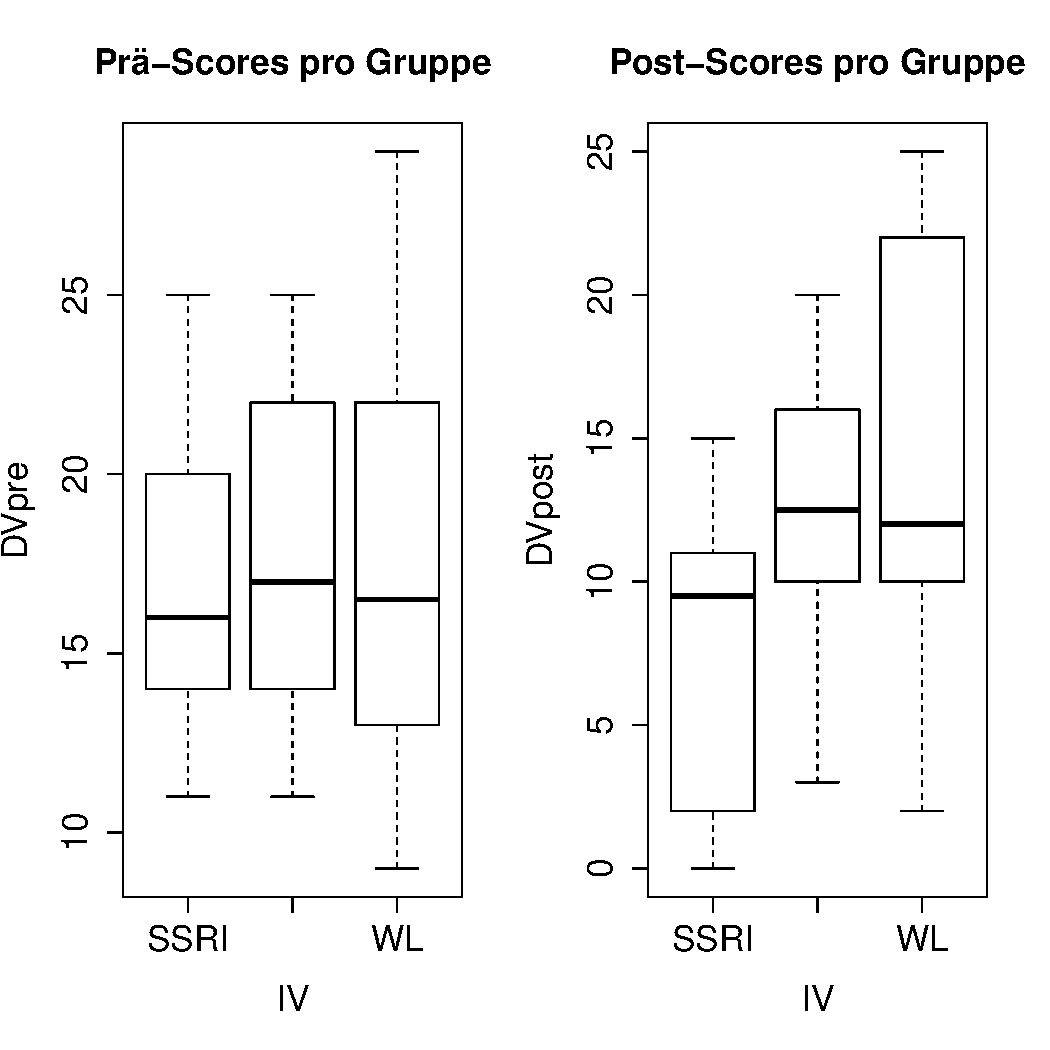
\includegraphics[width=8cm]{ancovaBoxplot}
\vspace*{-1em}
\caption{Kovarianzanalyse: Boxplots zum Vergleich der Verteilungen der Zielgröße in den Gruppen}
\label{fig:ancovaBoxplot}
\end{figure}

Zur Berechnung von Quadratsummen vom Typ III kann zum einen auf \lstinline!Anova()!\index[func]{Anova()@\lstinline{Anova()}} aus dem \lstinline!car!\index[pack]{car@\lstinline{car}} Paket zurückgegriffen werden.\footnote{Da keine Interaktion von Treatment-Variable und Kovariate berücksichtigt wird, sind die Quadratsummen vom Typ II und III hier identisch.} Zum anderen lassen sich diese Quadratsummen mit \lstinline!anova()! durch den Test zweier geeigneter Modelle gegeneinander ermitteln (Abschn.\ \ref{sec:ssTypes}): Für den Effekt der Kovariate sind dies auf der einen Seite das Modell ohne Kovariate als Vorhersageterm, auf der anderen Seite das vollständige Modell. Für den Effekt der Treatment-Variable entsprechend auf der einen Seite das Modell ohne Treatment-Variable als Vorhersageterm, auf der anderen Seite das vollständige Modell.
\begin{lstlisting}
# Effektcodierung für Quadratsummen vom Typ III
> fitFiii <- lm(DVpost ~ IV + DVpre,
+               contrasts=list(IV=contr.sum), data=dfAncova)

> library(car)                            # für Anova()
> Anova(fitFiii, type="III")              # QS Typ III
Anova Table (Type II tests)
Response: DVpost
             Sum Sq  Df  F value    Pr(>F)
(Intercept)   27.83   1   0.9567  0.337029
IV           217.15   2   3.7324  0.037584 *
DVpre        313.37   1  10.7723  0.002937 **
Residuals    756.33  26

# Quadratsummen vom Typ II (hier = III) über Modellvergleiche
> anova(fitRegr, fitFull)                 # Test Treatment ...
> anova(fitGrp,  fitFull)                 # Test Kovariate ...
\end{lstlisting}

Die Ergebnisse lassen sich manuell nachvollziehen, indem die Residual-Quadratsummen für das vollständige Modell, das Regressionsmodell ohne Treatment-Variable und das ANOVA-Modell ohne Kovariate berechnet werden. Die Effekt-Quadratsummen vom Typ III ergeben sich dann jeweils als Differenz der Residual-Quadratsumme des Modells, in dem dieser Effekt nicht berücksichtigt wird und der Residual-Quadratsumme des vollständigen Modells.
\begin{lstlisting}
> X   <- DVpre                            # kürzerer Name Kovariate
> Y   <- DVpost                           # kürzerer Name AV
> XMj <- tapply(X, IV, mean)              # Gruppenmittel Kovariate
> YMj <- tapply(Y, IV, mean)              # Gruppenmittel AV
> N   <- length(Y)                        # Gesamtanzahl Personen

# Residual-Quadratsumme vollständiges Modell
# zunächst gruppenweise zentrierte Daten der Kovariate und AV
> Xctr      <- X - ave(X, IV, FUN=mean)   # zentrierte Kovariate
> Yctr      <- Y - ave(Y, IV, FUN=mean)   # zentrierte AV
> bFull     <- cov(Xctr, Yctr) / var(Xctr)  # b-Gewicht (alle Gruppen)
> aFull     <- YMj - bFull*XMj            # y-Achsenabschnitte
> YhatFull  <- bFull*X + aFull[IV]        # Vorhersage
> SSEfull   <- sum((Y-YhatFull)^2)        # Residual-QS
> dfSSEfull <- N-P-1                      # Freiheitsgrade Residual-QS
> MSEfull   <- SSEfull / dfSSEfull        # mittlere Residual-QS

# Residual-Quadratsumme Regressionsmodell ohne Treatment-Variable
> bRegr     <- cov(X, Y) / var(X)         # b-Gewicht
> aRegr     <- mean(Y) - bRegr*mean(X)    # y-Achsenabschnitt
> YhatRegr  <- bRegr*X + aRegr            # Vorhersage
> SSEregr   <- sum((Y-YhatRegr)^2)        # Residual-QS
> dfSSEregr <- N-2                        # df Fehler
> MSEregr   <- SSEregr / dfSSEregr        # mittlere Residual-QS

# Residual-Quadratsumme ANOVA-Modell ohne Kovariate
> Vj       <- tapply(Y, IV, var)          # Gruppenvarianzen
> M        <- sum((Nj/N) * YMj)           # Gesamt-Mittel
> SSEgrp   <- sum((Nj-1) * Vj)            # Residual-QS
> dfSSEgrp <- N-P                         # df Fehler
> MSEgrp   <- SSEgrp / dfSSEgrp           # mittlere Residual-QS

# Effekt-Quadratsummen und F-Werte der zugehörigen Tests
> SSregr <- SSEgrp - SSEfull              # Effekt-QS Kovariate
> dfRegr <- dfSSEgrp - dfSSEfull          # df Kovariate -> 1
> MSregr <- SSregr / dfRegr               # MS Kovariate
> (Fregr <- MSregr / MSEfull)             # F-Wert Kovariate
[1] 10.77234

> SSgrp <- SSEregr - SSEfull              # Effekt-QS Treatment
> dfGrp <- dfSSEregr - dfSSEfull          # df Treatment -> P-1
> MSgrp <- SSgrp / dfGrp                  # MS Treatment
> (Fgrp <- MSgrp / MSEfull)               # F-Wert Treatment
[1] 3.732399
\end{lstlisting}

Mit \lstinline!summary(<<lm-Modell>>)!\index[func]{summary()@\lstinline{summary()}} lassen sich die in den verschiedenen Gruppen angepassten Regressionsparameter ausgeben und einzeln auf Signifikanz testen.
\begin{lstlisting}
> (sumRes <- summary(fitFull))            # gekürzte Ausgabe ...
Residuals:
     Min       1Q  Median      3Q     Max
-10.6842  -3.9615  0.6448  3.8773  9.9675

Coefficients:
             Estimate  Std. Error  t value  Pr(>|t|)
(Intercept)   -3.6704      3.7525   -0.978   0.33703
IVPlacebo      4.4483      2.4160    1.841   0.07703 .
IVWL           6.4419      2.4133    2.669   0.01292 *
DVpre          0.6453      0.1966    3.282   0.00294 **
---
Residual standard error: 5.393 on 26 degrees of freedom
Multiple R-squared: 0.4227,   Adjusted R-squared: 0.3561
F-statistic: 6.346 on 3 and 26 DF,  p-value: 0.002252
\end{lstlisting}

Die unter \lstinline!Coefficients! aufgeführten Testergebnisse sind so zu interpretieren, dass die SSRI-Gruppe als Referenzgruppe verwendet wurde, da sie die erste Faktorstufe in \lstinline!IV! darstellt (Abschn.\ \ref{sec:facLabelOrder}, \ref{sec:multALManova}). Ihre Koeffizienten finden sich in der Zeile \lstinline!(Intercept)!. Für diese Gruppe ist der unter \lstinline!Estimate! genannte Wert der $y$-Achsenabschnitt der Regressionsgerade. Die \lstinline!Estimate! Werte für die Gruppen \lstinline!Placebo! und \lstinline!WL! geben jeweils die Differenz des $y$-Achsenabschnitts in dieser Gruppe zur Referenzgruppe an. Der in der letzten Spalte genannte $p$-Wert gibt Auskunft auf die Frage, ob dieser Unterschied signifikant von $0$ verschieden ist. Die für alle Gruppen identische Steigung ist als \lstinline!Estimate! für die Kovariate \lstinline!DVpre! abzulesen. Ob sie signifikant von $0$ verschieden ist, ergibt sich aus dem in der letzten Spalte genannten $p$-Wert.\footnote{Die absolute Höhe der Gruppe der $y$-Achsenabschnitte lässt sich aus den Daten nicht unabhängig schätzen, während ihre Abstände untereinander eindeutig bestimmt sind. Die in \citeA[Kap.~9]{Maxwell2004} gezeigte Lösung fixiert den $y$-Achsenabschnitt der \lstinline!WL! Gruppe auf $0$ und berichtet die übrigen als Differenz dazu.}

Eine grafische Veranschaulichung des linearen Zusammenhangs zwischen Vorher- und Nachher-Messwert in den einzelnen Gruppen erfolgt in Abb.\ \ref{fig:ancovaRegr}.
\begin{lstlisting}
# Steigung und y-Achsenabschnitte der Regressionsgeraden extrahieren
> coeffs    <- coef(sumRes)                  # alle Koeffizienten
> iCeptSSRI <- coeffs[1, 1]                  # b0 SSRI (Referenzgruppe)
> iCeptPlac <- coeffs[2, 1] + iCeptSSRI      # b0 Placebo
> iCeptWL   <- coeffs[3, 1] + iCeptSSRI      # b0 Warteliste
> slopeAll  <- coeffs[4, 1]                  # gemeinsame Steigung

# Darstellungsbereich für x- & y-Achse wählen und Punktwolke darstellen
> xLims <- c(0, max(dfAncova$DVpre))
> yLims <- c(min(c(iCeptSSRI, iCeptPlac, iCeptWL)),
+            max(dfAncova$DVpost))

> plot(DVpost ~ DVpre, data=dfAncova, xlim=xLims, ylim=yLims,
+      pch=rep(c(3,17,19), Nj), col=rep(c("red", "green", "blue"), Nj),
+      main="Rohdaten und Regressionsgerade pro Gruppe")

> legend(x="topleft", legend=levels(IV), pch=c(3, 17, 19),
+        col=c("red", "green", "blue"))

# Regressionsgeraden einfügen
> abline(iCeptSSRI, slopeAll, col="red")
> abline(iCeptPlac, slopeAll, col="green")
> abline(iCeptWL,   slopeAll, col="blue")
\end{lstlisting}

\begin{figure}[ht]
\centering
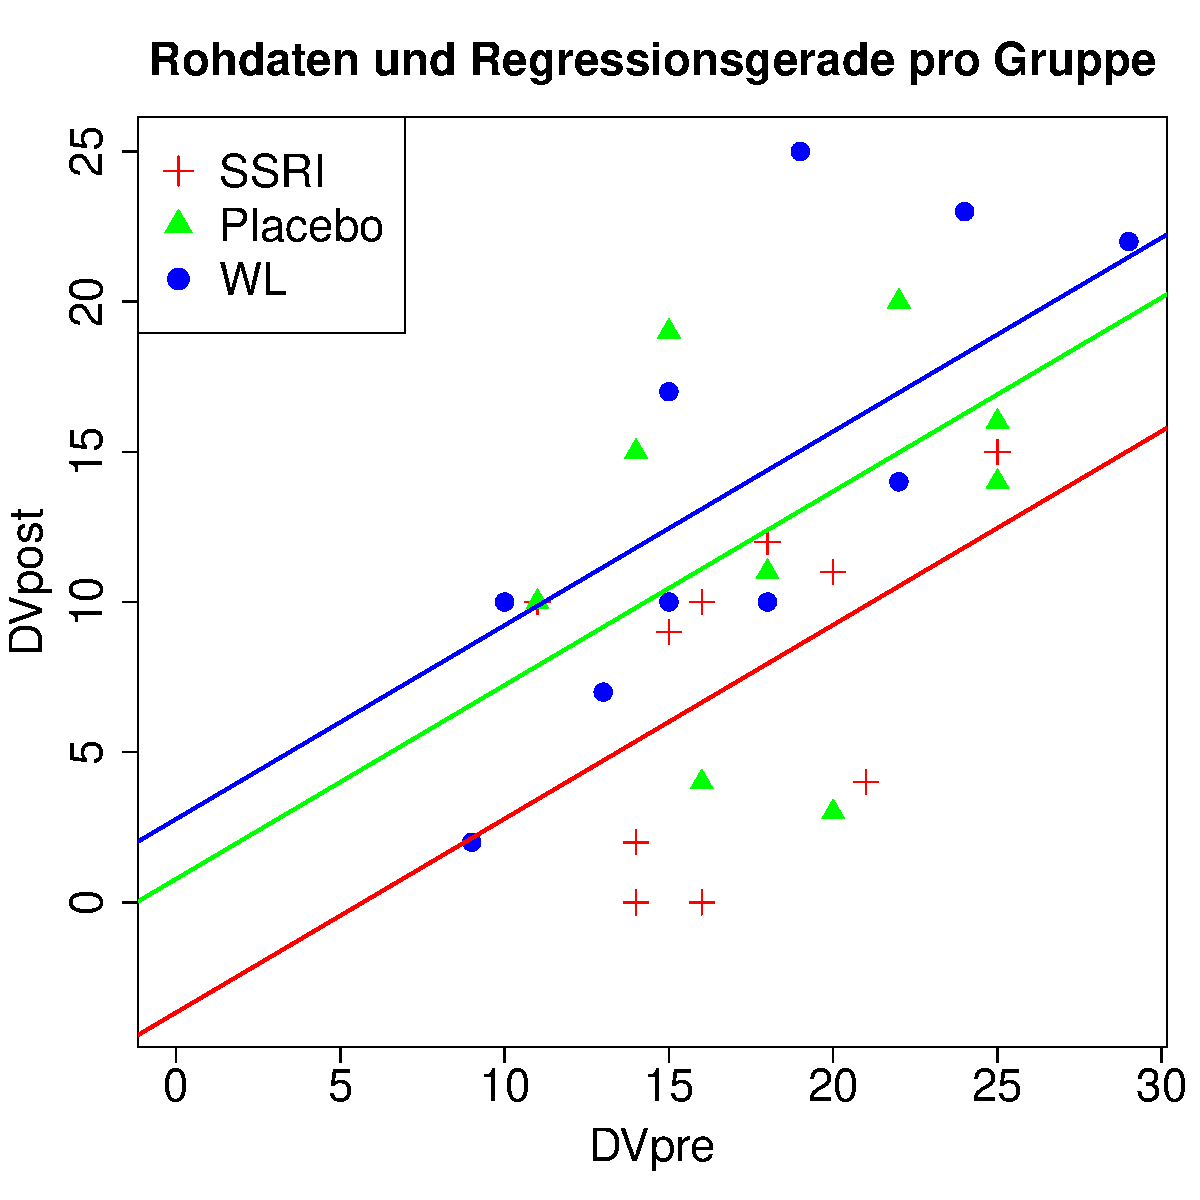
\includegraphics[width=8cm]{ancovaRegr}
\vspace*{-0.5em}
\caption{Kovarianzanalyse: nach Gruppen getrennte Regressionsgeraden}
\label{fig:ancovaRegr}
\end{figure}

\index{Kovarianzanalyse!Effektstärke}
\index{etaSq@$\hat{\eta}^{2}$ (Effektstärke)}
Als Maß für die Stärke jedes getesteten Effekts kann das partielle $\eta_{p}^{2}$ herangezogen werden, zu dessen Schätzung $\hat{\eta}_{p}^{2}$ jeweils seine Effekt-Quadratsumme an der Summe von ihr und der Residual-Quadratsumme relativiert wird. $\hat{\eta}_{p}^{2}$ der Kovariate ist hier gleich der quadrierten Partialkorrelation von Kovariate und Kriterium ohne die Treatment-Variable (Abschn.\ \ref{sec:partCorReg}).
\begin{lstlisting}
> SSEfull <- deviance(fitFull)         # Fehler-Quadratsumme full model
> SSEgrp  <- deviance(fitGrp)          # Fehler-Quadratsumme Treatment
> SSEregr <- deviance(fitRegr)         # Fehler-Quadratsumme Kovariate
> SSregr  <- SSEgrp  - SSEfull         # Effekt-Quadratsumme Kovariate
> SSgrp   <- SSEregr - SSEfull         # Effekt-Quadratsumme Treatment
> SSregr / (SSregr + SSEfull)          # partielles eta^2 Kovariate
[1] 0.2929469

# Kontrolle: Partialkorrelation Kovariate mit Kriterium ohne Faktor
> cor(residuals(lm(DVpre ~ IV)), residuals(lm(DVpost ~ IV)))^2
[1] 0.2929469

> SSgrp / (SSgrp + SSEfull)            # partielles eta^2 Treatment
[1] 0.2230642
\end{lstlisting}

Sollen in der Kovarianzanalyse die Steigungen der Regressionsgeraden in den Gruppen nicht als identisch festgelegt, sondern auch bzgl.\ dieses Parameters Gruppenunterschiede i.\,S.\ einer Moderation (Abschn.\ \ref{sec:regrMod}) zugelassen werden, lautet das Modell:
\begin{lstlisting}
> summary(lm(DVpost ~ IV + DVpre + IV:DVpre, data=dfAncova))      # ...
\end{lstlisting}

%%%%%%%%%%%%%%%%%%%%%%%%%%%%%%%%%%%%%%%%%%%%%%%%%%%%%%%%%%%%%%%%%%
%%%%%%%%%%%%%%%%%%%%%%%%%%%%%%%%%%%%%%%%%%%%%%%%%%%%%%%%%%%%%%%%%%
\subsection{Beliebige a-priori Kontraste}
%%%%%%%%%%%%%%%%%%%%%%%%%%%%%%%%%%%%%%%%%%%%%%%%%%%%%%%%%%%%%%%%%%
%%%%%%%%%%%%%%%%%%%%%%%%%%%%%%%%%%%%%%%%%%%%%%%%%%%%%%%%%%%%%%%%%%

\index{Kovarianzanalyse!Einzelvergleiche (Kontraste)}
Ähnlich wie bei Varianzanalysen lassen sich bei Kovarianzanalysen spezifische Vergleiche zwischen experimentellen Bedingungen in der Form von Kontrasten, also Linearkombinationen von Gruppenerwartungswerten testen (Abschn.\ \ref{sec:contrCRp}). Die Kovariate findet dabei Berücksichtigung, indem hier der Vergleich zwischen korrigierten Erwartungswerten der AV stattfindet: Auf empirischer Ebene müssen für deren Schätzung zunächst die Regressionsparameter pro Gruppe bestimmt werden, wobei wie oben das $b$-Gewicht konstant sein und nur die Variation des $y$-Achsenabschnitts zwischen den Gruppen zugelassen werden soll. Der Gesamtmittelwert der Kovariate über alle Gruppen hinweg wird nun pro Gruppe in die ermittelte Regressionsgleichung eingesetzt. Das Ergebnis ist der korrigierte Gruppenmittelwert, der ausdrücken soll, welcher Wert in der AV zu erwarten wäre, wenn alle Personen denselben Wert auf der Kovariate (nämlich deren Gesamtmittelwert) hätten und sich nur in der Gruppenzugehörigkeit unterscheiden würden.

\index[pack]{multcomp@\lstinline{multcomp}}
\index[func]{glht()@\lstinline{glht()}}
Im Beispiel werden drei Kontraste ohne $\alpha$-Adjustierung getestet. Dafür ist es notwendig, die zugehörigen Kontrastvektoren als (ggf.\ benannte) Zeilen einer Matrix zusammenzustellen.
\begin{lstlisting}
# Matrix der Kontrastkoeffizienten
> cntrMat <- rbind("SSRI-Placebo"   = c(-1, 1, 0),
+                  "SSRI-WL"        = c(-1, 0, 1),
+                  "SSRI-0.5(P+WL)" = c(-2, 1, 1))

> library(multcomp)                           # für glht()
> aovAncova <- aov(DVpost ~ IV + DVpre, data=dfAncova)
> (sumRes <- summary(glht(aovAncova, linfct=mcp(IV=cntrMat),
+                         alternative="greater"),
+                    test=adjusted("none")))
Simultaneous Tests for General Linear Hypotheses
Multiple Comparisons of Means: User-defined Contrasts
Fit: aov(formula = DVpost ~ IV + DVpre, data = dfAncova)
Linear Hypotheses:
                     Estimate  Std. Error  t value  Pr(>|t|)
SSRI-Placebo <= 0       4.448       2.416    1.841   0.03852 *
SSRI-WL <= 0            6.442       2.413    2.669   0.00646 **
SSRI-0.5(P+WL) <= 0    10.890       4.183    2.603   0.00753 **
\end{lstlisting}

Die korrigierten Gruppenmittel lassen sich mit \lstinline!interactionMeans(<<aov-Modell>>)!\index[func]{interactionMeans()@\lstinline{interactionMeans()}} aus dem Paket\index[pack]{phia@\lstinline{phia}} \lstinline!phia! berechnen.
\begin{lstlisting}
> library(phia)                               # für interactionMeans()
> interactionMeans(aovAncova)
       IV adjusted mean std. error
1    SSRI      7.536616   1.707096
2 Placebo     11.984895   1.706832
3      WL     13.978489   1.705586
\end{lstlisting}

Die Ergebnisse für korrigierte Gruppenmittel und Kontraste können manuell geprüft werden.
\begin{lstlisting}
> (YMjAdj <- bFull*mean(X) + aFull)           # korrig. Gruppenmittel
    SSRI    Placebo         WL 
7.536616  11.984895  13.978489

> psiHats    <- cntrMat     %*% YMjAdj        # Kontrastschätzungen
> lenSqs     <- cntrMat^2   %*% (1/Nj)        # quadrierte Längen
> Xctr       <- X - ave(X, IV, FUN=mean)      # zentrierte Kovariate
> fracs      <- (cntrMat %*% XMj)^2 / sum(Xctr^2)
> varPsiHats <- MSEfull * (lenSqs + fracs)    # Varianz der Schätzungen
> tStats     <- psiHats / sqrt(varPsiHats)    # Teststatistiken
> pVals      <- pt(abs(tStats), dfSSEfull, lower.tail=FALSE) # p-Werte
> data.frame(psiHats, tStats, pVals)
                  psiHats     tStats        pVals
SSRI-Placebo     4.448279  1.8411994  0.038515271
SSRI-WL          6.441874  2.6692923  0.006461541
SSRI-0.5(P+WL)  10.890153  2.6031958  0.007529061
\end{lstlisting}

%%%%%%%%%%%%%%%%%%%%%%%%%%%%%%%%%%%%%%%%%%%%%%%%%%%%%%%%%%%%%%%%%%
%%%%%%%%%%%%%%%%%%%%%%%%%%%%%%%%%%%%%%%%%%%%%%%%%%%%%%%%%%%%%%%%%%
\subsection{Beliebige post-hoc Kontraste nach Scheffé}
%%%%%%%%%%%%%%%%%%%%%%%%%%%%%%%%%%%%%%%%%%%%%%%%%%%%%%%%%%%%%%%%%%
%%%%%%%%%%%%%%%%%%%%%%%%%%%%%%%%%%%%%%%%%%%%%%%%%%%%%%%%%%%%%%%%%%

\index{Kovarianzanalyse!Einzelvergleiche (Kontraste)}
Beliebige Kontraste können auch im Anschluss an eine signifikante Kovarianzanalyse getestet werden, die implizit simultan alle möglichen Kontraste prüft -- spezifische Hypothesen liegen also bei ihrer Anwendung nicht vor. Aus diesem Grund muss im Anschluss an eine Kovarianzanalyse bei Einzeltests eine geeignete\index{alpha-Adjustierung@$\alpha$-Adjustierung} $\alpha$-Adjustierung vorgenommen werden, hier vorgestellt nach der Methode von Scheffé.

Zunächst gilt für das Aufstellen eines Kontrasts alles bereits für beliebige a-priori Kontraste Ausgeführte. Lediglich die Wahl des kritischen Wertes weicht ab und ergibt sich zur $\alpha$-Adjustierung aus einer $F$-Verteilung. Dieser kritische Wert ist mit dem Quadrat der a-priori $t$-Teststatistik zu vergleichen -- die etwa in der von \lstinline!summary(glht(...))! zurückgegebenen Liste in der Komponente \lstinline!test$tstat! steht. Hier sollen dieselben Kontraste wie im a-priori Fall gerichtet getestet werden.
\begin{lstlisting}
> dfSSgrp <- P-1                        # Freiheitsgrade Treatment-QS
> Fstats  <- sumRes$test$tstat^2        # quadrierte t-Teststatistiken

# p-Werte einseitig
> (pVals <- pf(Fstats/dfSSgrp, dfSSgrp, dfSSEfull, lower.tail=FALSE))
SSRI-Placebo      SSRI-WL  SSRI-0.5(P+WL)
  0.20326188   0.04291472      0.04923999
\end{lstlisting}

%%%%%%%%%%%%%%%%%%%%%%%%%%%%%%%%%%%%%%%%%%%%%%%%%%%%%%%%%%%%%%%%%%
%%%%%%%%%%%%%%%%%%%%%%%%%%%%%%%%%%%%%%%%%%%%%%%%%%%%%%%%%%%%%%%%%%
\section{Power, Effektstärke und notwendige Stichprobengröße}
\label{sec:power}
%%%%%%%%%%%%%%%%%%%%%%%%%%%%%%%%%%%%%%%%%%%%%%%%%%%%%%%%%%%%%%%%%%
%%%%%%%%%%%%%%%%%%%%%%%%%%%%%%%%%%%%%%%%%%%%%%%%%%%%%%%%%%%%%%%%%%

\index{power}
\index{Stichprobengrosse@Stichprobengröße}
\index{Fallzahlberechnung}
Mit Hilfe der Funktionen von Zufallsvariablen (Abschn.\ \ref{sec:randVarFuncs}) lässt sich die power der vorgestellten inferenzstatistischen Tests berechnen, sofern eine exakte $\text{H}_{1}$ vorliegt. Hierfür ist es notwendig, zunächst auf Basis der Verteilung der Teststatistik unter $\text{H}_{0}$ mit der Quantilfunktion \lstinline!q<<Funktionsfamilie>>()! den kritischen Wert für das gewünschte $\alpha$-Niveau zu bestimmen. Mit Hilfe der zugehörigen Verteilungsfunktion \lstinline!p<<Funktionsfamilie>>()! kann dann unter Gültigkeit der $\text{H}_{1}$ die power berechnet werden.

Analog lässt sich auch die notwendige Stichprobengröße (Fallzahl) ermitteln, für die der Test bei einem als gegeben vorausgesetzten Effekt eine gewisse power erreicht. Hierfür bedarf es meist eines Nonzentralitätsparameters der Verteilung der Teststatistik unter $\text{H}_{1}$, der anhand der aus der Statistik bekannten Formeln zu berechnen ist und sich aus der theoretischen Effektstärke ergibt.

Die im Basisumfang von R enthaltenen Funktionen zur Bestimmung von power und Stichprobengröße besitzen eine recht eingeschränkte Funktionalität, so berücksichtigen sie nur Binomialtest, $t$-Test und Varianzanalyse. Mehr Möglichkeiten bieten die Pakete \lstinline!pwr!\index[pack]{pwr@\lstinline{pwr}} \cite{Champely2007} und\index[pack]{MBESS@\lstinline{MBESS}} \lstinline!MBESS!. Insbesondere besitzt jedoch das kostenlose Programm G*Power \cite{Faul2007} einen deutlich breiteren Einsatzbereich hinsichtlich der unterstützten Tests. Zudem bietet es vielfältige Möglichkeiten zur Visualisierung der Zusammenhänge von Effektstärke, power und Fallzahl.

%%%%%%%%%%%%%%%%%%%%%%%%%%%%%%%%%%%%%%%%%%%%%%%%%%%%%%%%%%%%%%%%%%
%%%%%%%%%%%%%%%%%%%%%%%%%%%%%%%%%%%%%%%%%%%%%%%%%%%%%%%%%%%%%%%%%%
\subsection{Binomialtest}
%%%%%%%%%%%%%%%%%%%%%%%%%%%%%%%%%%%%%%%%%%%%%%%%%%%%%%%%%%%%%%%%%%
%%%%%%%%%%%%%%%%%%%%%%%%%%%%%%%%%%%%%%%%%%%%%%%%%%%%%%%%%%%%%%%%%%

\index{Binomialtest!power}
Im Beispiel soll zunächst der Fall eines rechtsseitigen Binomialtests betrachtet werden (Abschn.\ \ref{sec:binomTest}). Die Punktwahrscheinlichkeiten der einzelnen Ereignisse bei Gültigkeit von $\text{H}_{0}$ und $\text{H}_{1}$ sind zusammen mit dem kritischen Wert in Abb.\ \ref{fig:powerBinom} dargestellt.
\begin{lstlisting}
> N      <- 7                 # Stichprobengröße
> pH0    <- 0.25              # Wahrscheinlichkeit Treffer unter H0
> pH1    <- 0.7               # Wahrscheinlichkeit Treffer unter H1
> alpha  <- 0.05              # Signifikanzniveau
> (critB <- qbinom(alpha, N, pH0, lower.tail=FALSE))  # krit. Wert
[1] 4

# power für konkrete H0, H1, N
> (powB <- pbinom(critB, N, pH1, lower.tail=FALSE))
[1] 0.6470695

> sum(dbinom((critB+1):N, N, pH1))    # Kontrolle: Summe Einzelwkt.
[1] 0.6470695

# Säulendiagramm: Veranschaulichung der Wahrscheinlichkeitsfunktionen
> dH0 <- dbinom(0:N, N, pH0)          # Verteilung unter H0
> dH1 <- dbinom(0:N, N, pH1)          # Verteilung unter H1
> mat <- rbind(dH0, dH1)
> rownames(mat) <- c("H0 (p=0.25)", "H1 (p=0.7)")
> colnames(mat) <- 0:N
> barsX <- barplot(mat, beside=TRUE, ylim=c(0, 0.35),
+              xlab="Anzahl Treffer", ylab="Wahrscheinlichkeit",
+              main="Binomialvert. unter H0 und H1 (N=7)",
+              col=c(rgb(1, 0.2, 0.2, 0.7), rgb(0.3, 0.3, 1, 0.6))),
+              names.arg=colnames(mat), legend.text=rownames(mat))

> barplot(mat[ , 1:(critB+1)], beside=TRUE, ylim=c(0, 0.35),
+         col=c("red", "blue"), add=TRUE)

# Hilfslinie für kritischen Wert
> xx <- barsX[2, critB+1] + (barsX[1, critB+2] - barsX[2, critB+1]) / 4
> abline(v=xx, col="green", lwd=2)
> text(xx-0.4, 0.34, adj=1, labels="kritischer Wert")
\end{lstlisting}

Beim Test mit der diskreten Binomialverteilung ist die power keine monotone Funktion der Stichprobengröße, sondern kann auch sinken, wenn der Test bei fester $\text{H}_{0}$ und $\text{H}_{1}$ mit Daten von mehr Beobachtungsobjekten durchgeführt wird. Dies liegt an der Veränderung des kritischen Wertes, die zusammen mit der Powerfunktion in Abb.\ \ref{fig:powerBinom} abgebildet ist.
\begin{lstlisting}
> Nvec <- 2:15                          # betrachteter Bereich für N

# kritische Werte
> critBvec <- qbinom(alpha,    size=Nvec, prob=pH0, lower.tail=FALSE)

# power
> powBvec  <- pbinom(critBvec, size=Nvec, prob=pH1, lower.tail=FALSE)

# veranschauliche Verlauf der kritischen Werte
> par(mar=c(5, 4, 4, 4))                # breiterer rechter Rand
> plot(Nvec, critBvec, xlab="N", xaxt="n", yaxt="n", lwd=2, type="s",
+      pch=16, col="red", main="Power und kritischer Wert
+      Binomialtest", ylab="kritischer Wert")

# zeichne Achsen separat ein
> axis(side=1, at=seq(Nvec[1], Nvec[length(Nvec)], by=1))
> axis(side=2, at=seq(min(critBvec), max(critBvec), by=1), col="red")
> par(new=TRUE)                         # füge Powerfunktion hinzu
> plot(Nvec, powBvec, ylim=c(0, 1), type="b", lwd=2, pch=16,
+      col="blue", xlab=NA, ylab=NA, axes=FALSE)

# zeichne rechte Achse mit Achsenbeschriftung separat ein
> axis(side=4, at=seq(0, 1, by=0.1), col="blue")
> mtext(text="Power", side=4, line=3, cex=1.4)
\end{lstlisting}

\begin{figure}[ht]
\centering
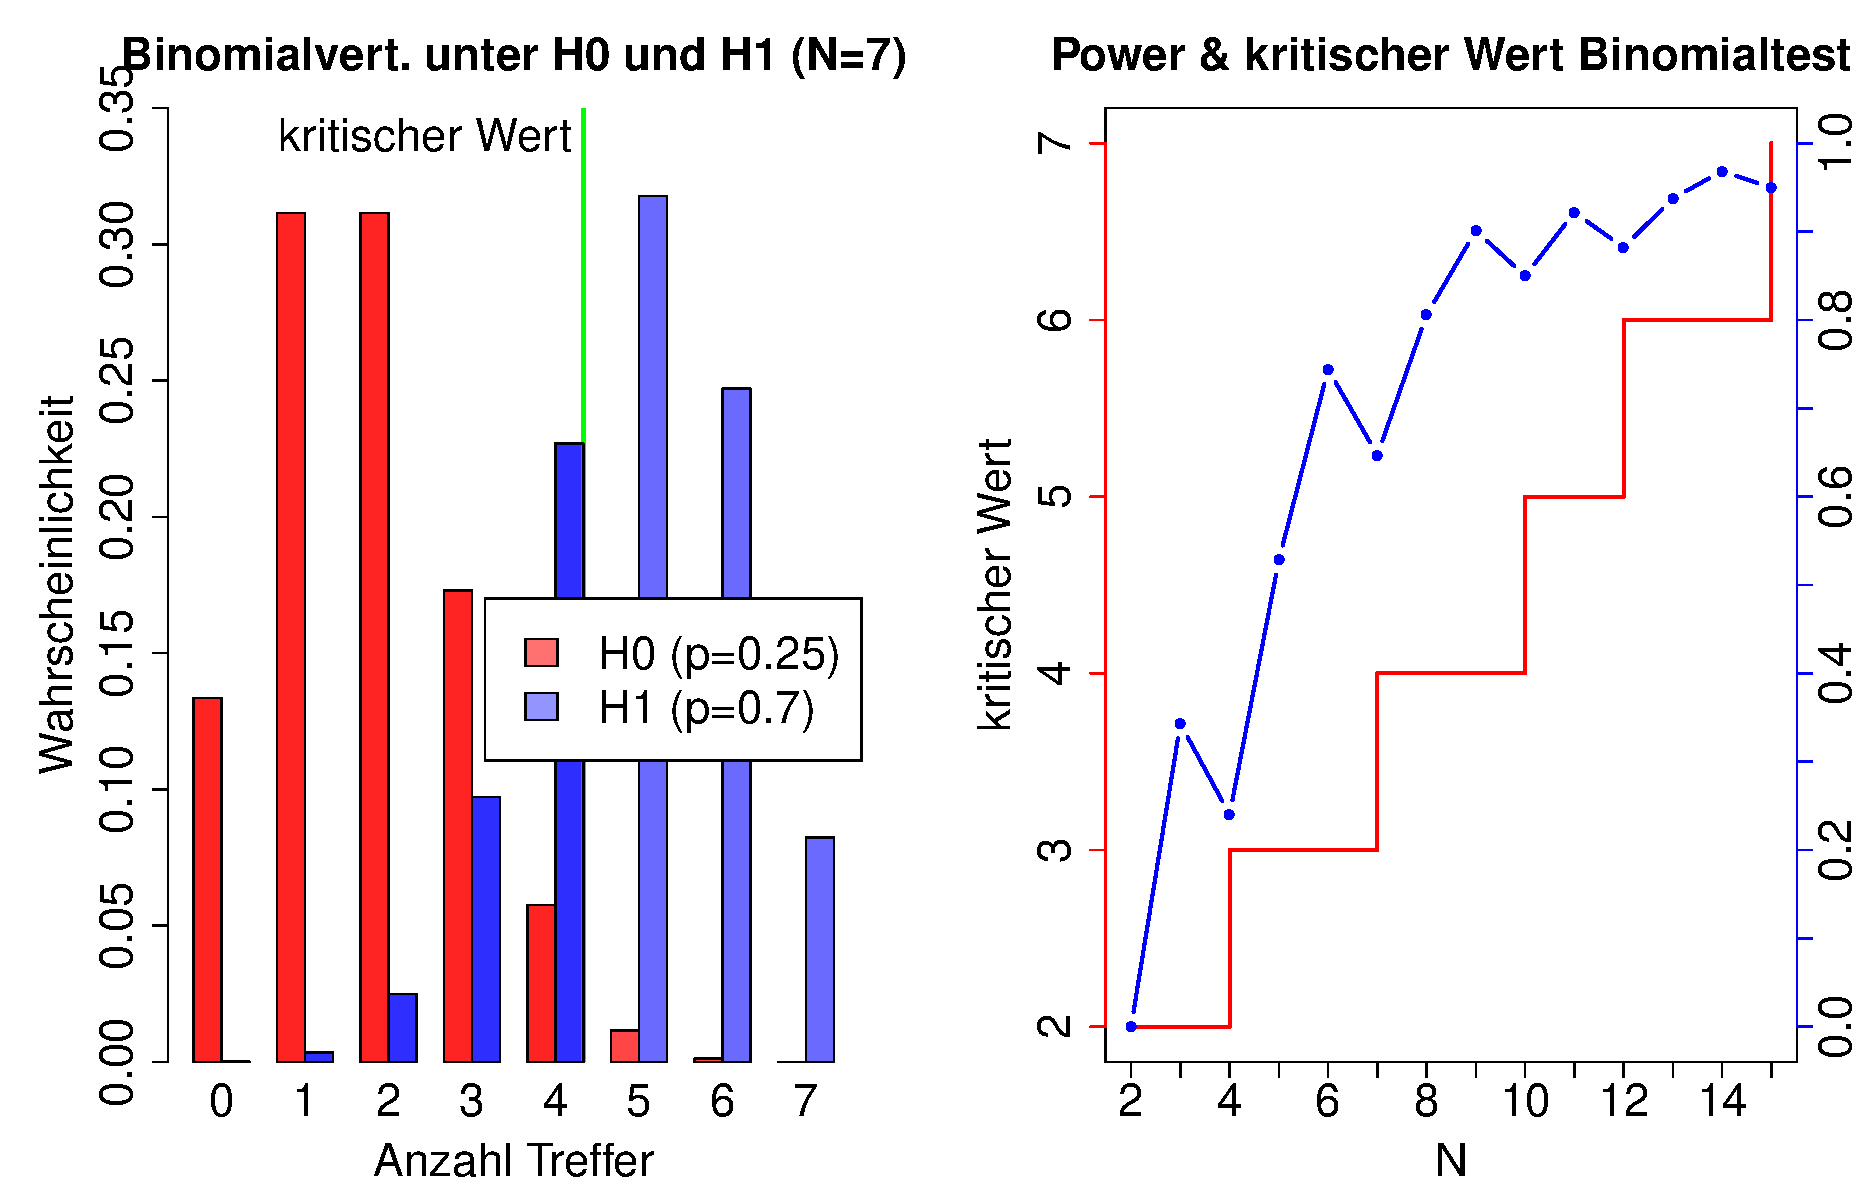
\includegraphics[width=12.5cm]{powerBinom}
\vspace*{-0.5em}
\caption{Binomialverteilung: Wahrscheinlichkeiten von Treffern unter $\text{H}_{0}$ und $\text{H}_{1}$ sowie kritischer Wert. Powerfunktion und kritischer Wert in Abhängigkeit von der Stichprobengröße}
\label{fig:powerBinom}
\end{figure}

%%%%%%%%%%%%%%%%%%%%%%%%%%%%%%%%%%%%%%%%%%%%%%%%%%%%%%%%%%%%%%%%%%
%%%%%%%%%%%%%%%%%%%%%%%%%%%%%%%%%%%%%%%%%%%%%%%%%%%%%%%%%%%%%%%%%%
\subsection[\texorpdfstring{$t$}{t}-Test]{$\bm{t}$-Test}
%%%%%%%%%%%%%%%%%%%%%%%%%%%%%%%%%%%%%%%%%%%%%%%%%%%%%%%%%%%%%%%%%%
%%%%%%%%%%%%%%%%%%%%%%%%%%%%%%%%%%%%%%%%%%%%%%%%%%%%%%%%%%%%%%%%%%

\index{t-Test@$t$-Test!power}
Für den $t$-Test mit einer Stichprobe ist zur Bestimmung der Verteilung der Teststatistik unter $\text{H}_{1}$ die Berechnung des\index{Verteilung!Nonzentralitätsparameter} Nonzentralitätsparameters $\delta$ erforderlich, für den die theoretische Streuung sowie der Erwartungswert unter $\text{H}_{0}$ und $\text{H}_{1}$ bekannt sein muss.\footnote{Für zwei unabhängige Stichproben mit Gruppengrößen $n_{1}$ und $n_{2}$, Streuung $\sigma$ und Erwartungswerten $\mu_{1}$ und $\mu_{2}$ unter $\text{H}_{1}$ ist $\delta = \sqrt{\frac{n_{1} \, n_{2}}{n_{1}+n_{2}}} \, \frac{\mu_{2}-\mu_{1}}{\sigma}$. Für zwei abhängige Stichproben des jeweiligen Umfangs $n$ mit theoretischen Streuungen $\sigma_{1}$ und $\sigma_{2}$ sowie der theoretischen Korrelation $\rho$ ist $\delta = \sqrt{n} \, \frac{\mu_{2}-\mu_{1}}{\sqrt{\sigma_{1}^{2} + \sigma_{2}^{2} + 2 \, \rho \, \sigma_{1} \, \sigma_{2}}}$.} Abbildung \ref{fig:powerT} zeigt die Verteilungen von $t$ für das gegebene Hypothesenpaar und kennzeichnet die Flächen, deren Größe $\alpha$, $\beta$ und power bei einem rechtsseitigen Test entsprechen.
\begin{lstlisting}
> N     <- 10                                 # Stichprobengröße
> muH0  <- 0                                  # Erwartungswert unter H0
> muH1  <- 1.6                                # Erwartungswert unter H1
> alpha <- 0.05                               # Signifikanzniveau
> sigma <- 2                                  # theoretische Streuung
> (d    <- (muH1-muH0) / sigma)               # Effektstärke d
[1] 0.8

> (delta <- (muH1-muH0) / (sigma/sqrt(N)))    # NZP, oder: sqrt(N)*d
[1] 2.529822

> (tCrit <- qt(1-alpha, N-1, lower.tail=FALSE))     # kritischer t-Wert
[1] 1.833113

> (powT <- pt(tCrit, N-1, delta, lower.tail=FALSE)) #  power
[1] 0.7544248

# bestimme Werte der t-Verteilungen
> xLims  <- c(-5, 10)
> tLeft  <- seq(xLims[1], tCrit, length.out=100)
> tRight <- seq(tCrit, xLims[2], length.out=100)
> yH0r   <- dt(tRight, N-1, 0)
> yH1l   <- dt(tLeft,  N-1, delta)
> yH1r   <- dt(tRight, N-1, delta)

# markiere Flächen für alpha, beta und power
> curve(dt(x, N-1, 0), xlim=xLims, lwd=2, col="red", xlab="t",
+       ylab="Dichte", main="Verteilung von t unter H0 und H1",
+       ylim=c(0, 0.4), xaxs="i")

> curve(dt(x, N-1, delta), lwd=2, col="blue", add=TRUE)
> polygon(c(tRight, rev(tRight)), c(yH0r, numeric(length(tRight))),
+         border=NA, col=rgb(1, 0.3, 0.3, 0.6))

> polygon(c(tLeft, rev(tLeft)), c(yH1l, numeric(length(tLeft))),
+         border=NA, col=rgb(0.3, 0.3, 1, 0.6))

> polygon(c(tRight, rev(tRight)), c(yH1r, numeric(length(tRight))),
+         border=NA, density=5, lty=2, lwd=2, angle=45, col="darkgray")

# zusätzliche Beschriftungen
> abline(v=tCrit, lty=1, lwd=3, col="red")
> text(tCrit+0.2, 0.4,  adj=0, labels="kritischer Wert")
> text(tCrit-2.8, 0.3,  adj=1, labels="Verteilung unter H0")
> text(tCrit+1.5, 0.3,  adj=0, labels="Verteilung unter H1")
> text(tCrit+1.0, 0.08, adj=0, labels="Power")
> text(tCrit-0.7, 0.05,  expression(beta))
> text(tCrit+0.5, 0.015, expression(alpha))
\end{lstlisting}

\begin{figure}[ht]
\centering
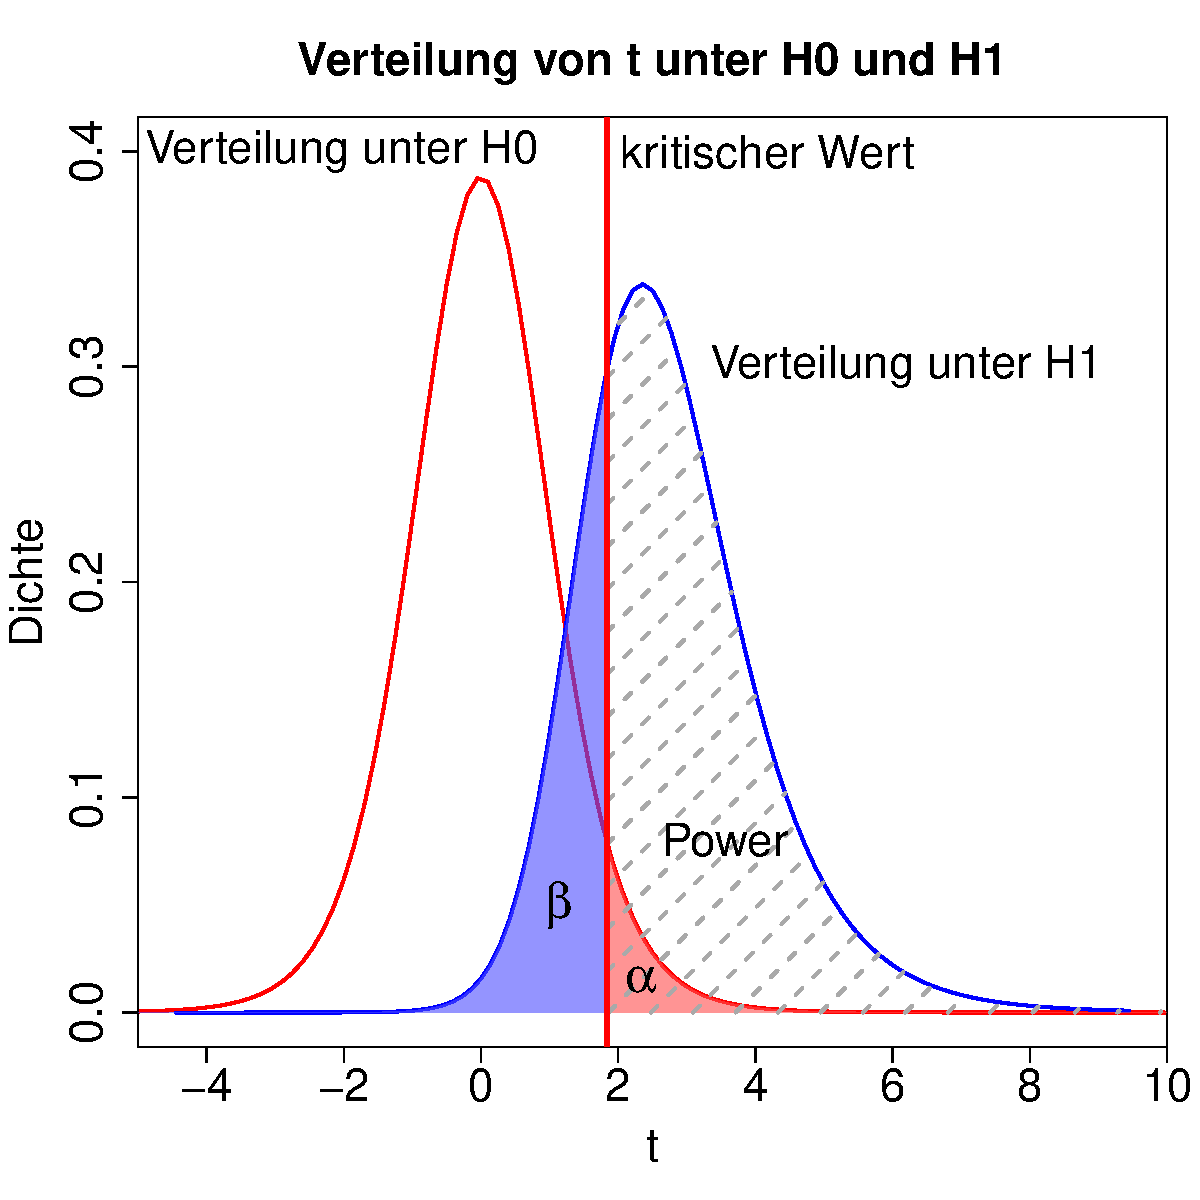
\includegraphics[width=8cm]{powerT}
\vspace*{-1em}
\caption{Rechtsseitiger $t$-Test für eine Stichprobe: Verteilung von $t$ unter $\text{H}_{0}$ und $\text{H}_{1}$, kritischer Wert, $\alpha$, $\beta$ und power}
\label{fig:powerT}
\end{figure}

\index{t-Test@$t$-Test!power}
\index{t-Test@$t$-Test!Stichprobengröße}
Wie für Binomial- und $t$-Tests demonstriert, kann die power analog für viele andere Tests manuell ermittelt werden. Für die Berechnung der power von $t$-Tests, bestimmten $\chi^{2}$-Tests und einfaktoriellen Varianzanalysen ohne Messwiederholung stehen in R auch eigene Funktionen bereit, deren Name nach dem Muster \lstinline!power.<<Test>>.test()! aufgebaut ist. Diese Funktionen dienen gleichzeitig der Ermittlung der Stichprobengröße, die notwendig ist, damit ein Test bei fester Effektstärke eine vorgegebene Mindest-Power\index[func]{power.t.test()@\lstinline{power.t.test()}} erzielt.\footnote{Die Funktionen sind nicht vektorisiert, akzeptieren für jedes Argument also nur jeweils einen Wert.}
\begin{lstlisting}
power.t.test(n, delta, sd, sig.level, power, strict=FALSE,
             type=c("two.sample, "one.sample", "paired"),
             alternative=c("two.sided", "one.sided"))
\end{lstlisting}

Von den Argumenten \lstinline!n! für die Gruppengröße, \lstinline!delta! für die Differenz der Erwartungswerte unter $\text{H}_{0}$ und $\text{H}_{1}$, \lstinline!sd! für die theoretische Streuung, \lstinline!sig.level! für das $\alpha$-Niveau und \lstinline!power! für die power sind genau vier mit konkreten Werten zu nennen und eines auf \lstinline!NULL! zu setzen. Das auf \lstinline!NULL! gesetzte Argument wird dann auf Basis der übrigen berechnet. \lstinline!n! bezieht sich im Fall zweier Stichproben auf die Größe jeder Gruppe -- es werden also auch bei unabhängigen Stichproben gleiche Gruppengrößen vorausgesetzt.\footnote{Für unterschiedliche Gruppengrößen $n_{1}$ und $n_{2}$ lassen sich annähernd richtige Ergebnisse erzielen, wenn \lstinline!2*((n1*n2)/(n1+n2))! für das Argument \lstinline!n! übergeben wird, wodurch die Berechnung des\index{Verteilung!Nonzentralitätsparameter} Nonzentralitätsparameters $\delta$ als \lstinline!sqrt(n/2) * (delta/sd)! korrekt ist. Statt mit der richtigen Zahl der Freiheitsgrade $n_{1}+n_{2}-2$ rechnet \lstinline!power.t.test()! dann aber mit $4 \, \frac{n_{1} \, n_{2}}{n_{1}+n_{2}} - 2$. Der so entstehende Fehler wächst zwar mit der Differenz von $n_{1}$ und $n_{2}$, bleibt jedoch absolut gesehen gering.}

Welche Art von $t$-Test vorliegt, kann über \lstinline!type! angegeben werden, \lstinline!alternative! legt fest, ob die $\text{H}_{1}$ gerichtet oder ungerichtet ist. Das Argument \lstinline!strict! bestimmt, ob im zweiseitigen Test für die power die Wahrscheinlichkeit berücksichtigt werden soll, auch auf der falschen Seite (relativ zur Lage der tatsächlichen Verteilung unter $\text{H}_{1}$) die $\text{H}_{0}$ zu verwerfen.

Eine Fragestellung für den Einsatz von \lstinline!power.t.test()! ist die Aufgabe, eine Stichprobengröße zu ermitteln, für die der Test bei einem als gegeben vorausgesetzten Effekt eine gewisse power erreicht. In diesem Fall ist also das Argument \lstinline!n=NULL! zu übergeben, alle anderen sind zu spezifizieren. Die ausgegebene Gruppengröße ist i.\,d.\,R.\ nicht ganzzahlig, muss also in der konkreten Anwendung aufgerundet werden, wodurch sich die tatsächliche power des Tests leicht erhöht.

Im Beispiel soll für die oben gegebene Situation herausgefunden werden, wie viele Beobachtungsobjekte notwendig sind, damit der Test eine power von $0.9$ besitzt.
\begin{lstlisting}
> power.t.test(n=NULL, delta=muH1-muH0, sd=sigma, sig.level=0.05,
+              power=0.9, type="one.sample", alternative="one.sided")
One-sample t test power calculation
          n = 14.84346
      delta = 1.6
         sd = 2
  sig.level = 0.05
      power = 0.9
alternative = one.sided
\end{lstlisting}

Eine andere Frage ist, wie groß bei einer gegebenen Stichprobengröße der tatsächliche Effekt sein muss, damit der Test eine bestimmte power erreicht. Hier ist \lstinline!delta=NULL! zu übergeben, alle anderen Argumente sind zu spezifizieren.

%%%%%%%%%%%%%%%%%%%%%%%%%%%%%%%%%%%%%%%%%%%%%%%%%%%%%%%%%%%%%%%%%%
%%%%%%%%%%%%%%%%%%%%%%%%%%%%%%%%%%%%%%%%%%%%%%%%%%%%%%%%%%%%%%%%%%
\subsection{Einfaktorielle Varianzanalyse}
\label{sec:powerAnova}
%%%%%%%%%%%%%%%%%%%%%%%%%%%%%%%%%%%%%%%%%%%%%%%%%%%%%%%%%%%%%%%%%%
%%%%%%%%%%%%%%%%%%%%%%%%%%%%%%%%%%%%%%%%%%%%%%%%%%%%%%%%%%%%%%%%%%

\index{Varianzanalyse!power}
\index{Varianzanalyse!Stichprobengröße}
Die analog zu \lstinline!power.t.test()! arbeitende Funktion für eine einfaktorielle Varianzanalyse ohne Messwiederholung lautet\index[func]{power.anova.test()@\lstinline{power.anova.test()}} \lstinline!power.anova.test()!.
\begin{lstlisting}
power.anova.test(groups, n, between.var, within.var, sig.level, power)
\end{lstlisting}

Von den Argumenten \lstinline!groups! für die Anzahl der Gruppen, \lstinline!n! für die Gruppengröße, \lstinline!between.var! für die Varianz der Erwartungswerte unter $\text{H}_{1}$,\footnote{Enthält der Vektor \lstinline!muJ! die Erwartungswerte der Gruppen unter $\text{H}_{1}$, muss wegen der in \lstinline!power.anova.test()! verwendeten Formel für den Nonzentralitätsparameter $\lambda$ die korrigierte Varianz der Erwartungswerte, also \lstinline!var(muJ)!, für das Argument \lstinline!between.var! übergeben werden.} \lstinline!within.var! für die theoretische Fehlervarianz, \lstinline!sig.level! für den $\alpha$-Fehler und \lstinline!power! für die power sind genau fünf mit konkreten Werten zu nennen und eines auf \lstinline!NULL! zu setzen. Das auf \lstinline!NULL! gesetzte Argument wird dann auf Basis der übrigen berechnet. \lstinline!n! bezieht sich auf die Größe jeder Gruppe -- es werden also gleiche Gruppengrößen vorausgesetzt.

Im folgenden Beispiel einer einfaktoriellen Varianzanalyse ohne Messwiederholung soll die notwendige Stichprobengröße berechnet werden, damit der Test bei gegebenen Erwartungswerten unter $\text{H}_{1}$ eine bestimmte power erzielt.
\begin{lstlisting}
> muJ   <- c(100, 110, 115)               # Erwartungswerte unter H1
> sigma <- 15                             # theoretische Streuung
> power.anova.test(groups=3, n=NULL, between.var=var(muJ),
+                  within.var=sigma^2, sig.level=0.05, power=0.9)
Balanced one-way analysis of variance power calculation
     groups = 3
          n = 25.4322
between.var = 58.33333
 within.var = 225
  sig.level = 0.05
      power = 0.9

NOTE: n is number in each group
\end{lstlisting}

Für das gegebene Beispiel folgt die manuelle Berechnung der power und der Maße für die Effektstärke einer Varianzanalyse im CR-$p$ Design mit ungleichen Zellbesetzungen\index{Verteilung!Nonzentralitätsparameter}.
\begin{lstlisting}
> P      <- length(muJ)           # Anzahl Gruppen
> Nj     <- c(21, 17, 19)         # Gruppengrößen
> N      <- sum(Nj)               # Gesamt-N
> mu     <- sum(Nj * muJ) / N     # mittlerer Erwartungswert, gewichtet
> alphaJ <- muJ - mu              # Gruppeneffekte
> varMUj <- sum(Nj * alphaJ^2)/N  # Varianz der Erwartungswerte

# Maße für die Effektstärke - Bezeichnungen uneinheitlich
> (fSq <- varMUj / sigma^2)                 # f^2
[1] 0.1826887

> (etaSq <- varMUj / (sigma^2 + varMUj))    # eta^2 bzw. omega^2
[1] 0.1544690

# Nonzentralitätsparam. lambda bzw. delta^2 - Bezeichnung uneinheitlich
> (lambda <- sum(Nj * alphaJ^2) / sigma^2)  # oder: N * fSq
[1] 10.41326

# kritischer Wert, alpha=0.05
> (Fcrit <- qf(0.05, P-1, N-P, lower.tail=FALSE))
[1] 3.168246

> (powF <- pf(Fcrit, P-1, N-P, lambda, lower.tail=FALSE))   # power
[1] 0.8090387
\end{lstlisting}

Liegt keine exakte $\text{H}_{1}$ vor, ist die power als Funktion der Effektstärke $f$ darstellbar (Abb.\ \ref{fig:powerFunc}).

\begin{figure}[ht]
\centering
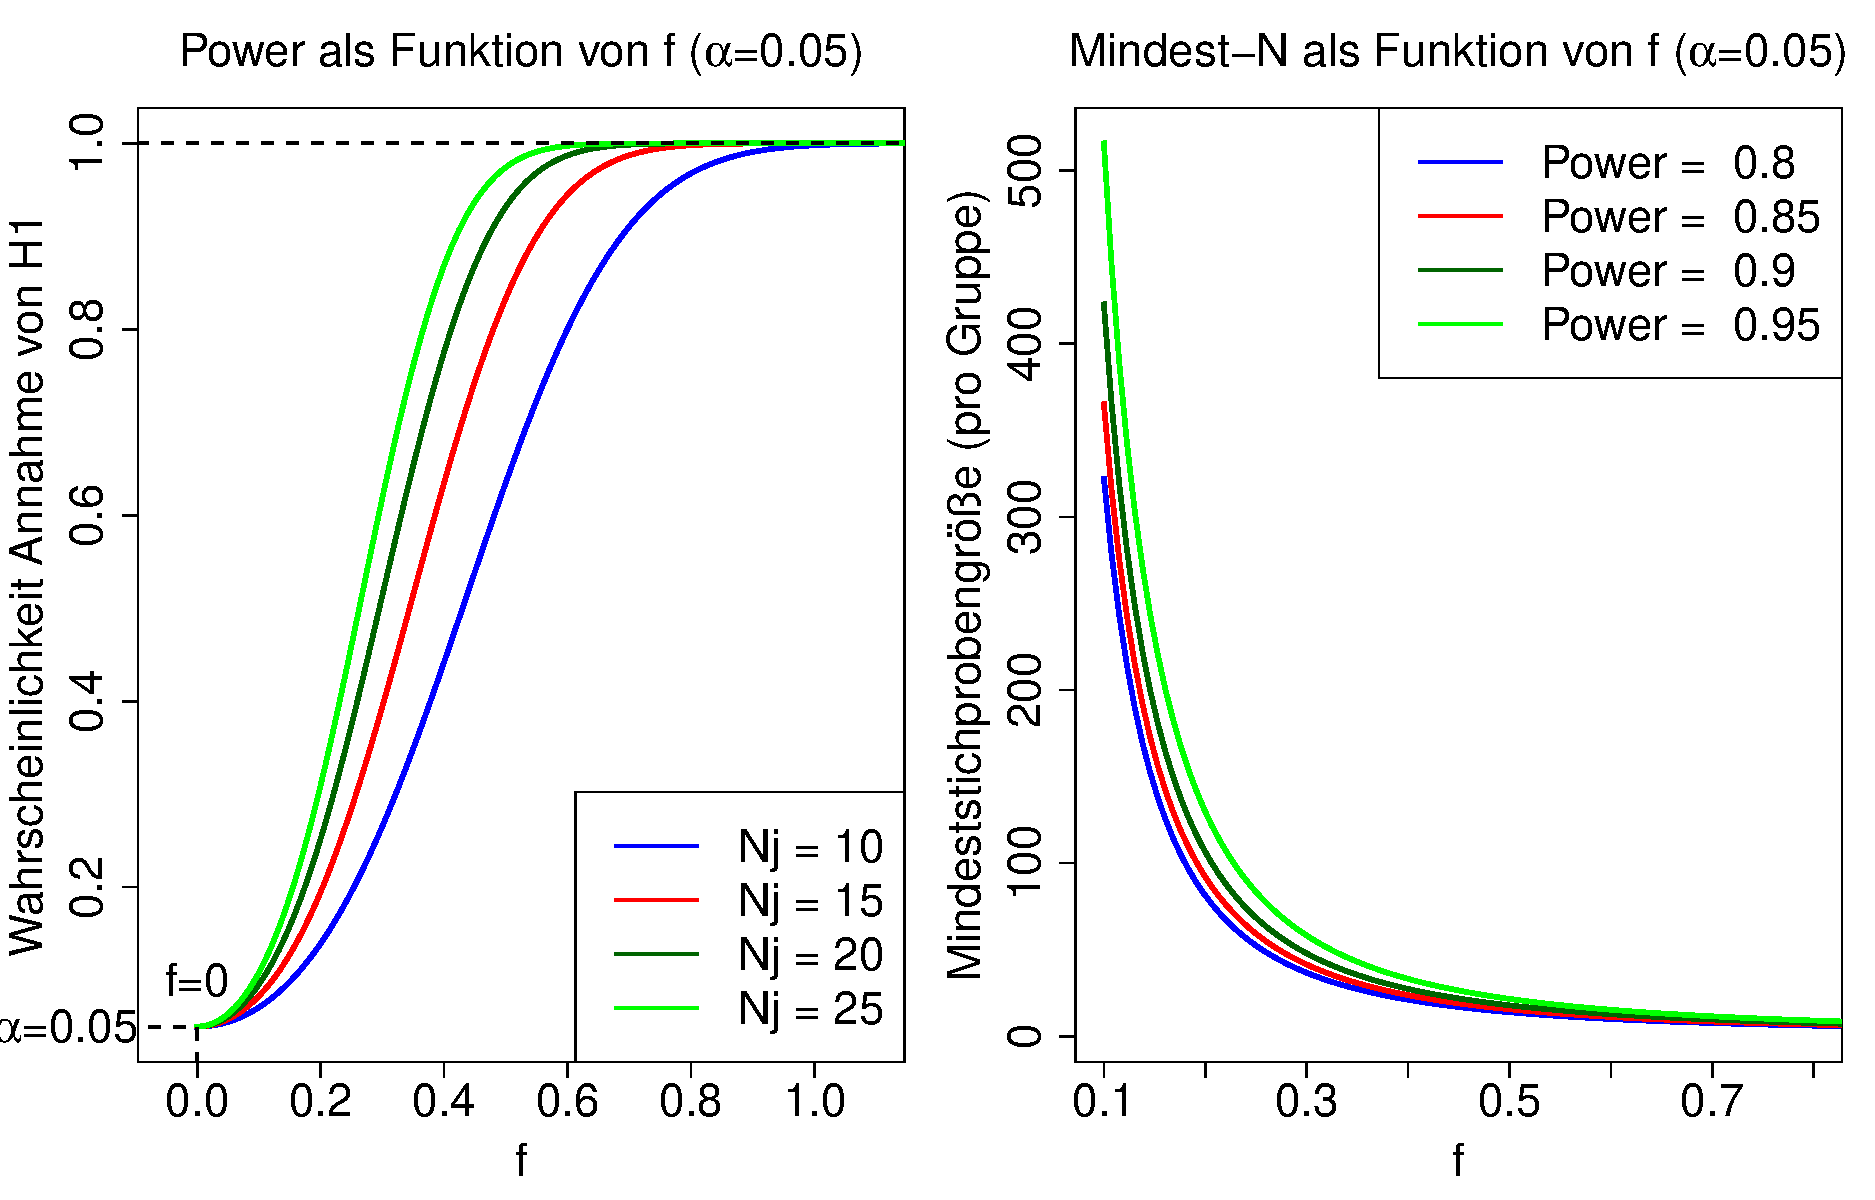
\includegraphics[width=12.5cm]{powerFunc}
\vspace*{-0.5em}
\caption{Einfaktorielle Varianzanalyse: power als Funktion der Effektstärke $f$ für verschiedene Gruppengrößen sowie Mindeststichprobengröße als Funktion von $f$ für verschiedene Power-Werte}
\label{fig:powerFunc}
\end{figure}

\begin{lstlisting}
> fVals <- seq(0, 1.2, length.out=100)    # Effektstärken f auf x-Achse
> nn    <- seq(10, 25, by=5)    # Stichprobengrößen: separate Kurven

# Funktion: power für verschiedene Stichprobengrößen und f-Werte
> getFpow <- function(n) {
+     Fcrit <- qf(0.05, P-1, P*n - P, lower.tail=FALSE)
+     pf(Fcrit, P-1, P*n - P, P*n * fVals^2, lower.tail=FALSE)
+ }

> powsF <- sapply(nn, getFpow)  # Power-Werte für jede Stichprobengröße

# Beschriftungen vorbereiten
> yStr <- "Wahrscheinlichkeit der Annahme von H1"
> mStr <- substitute(paste("Power - Funktion von f (",alpha,"=0.05)"))

# Power-Werte darstellen
> matplot(fVals, powsF, type="l", lty=1, lwd=2, xlab="f", ylab=yStr,
+         xlim=c(-0.05, 1.1), main=mStr,
+         col=c("blue", "red", "darkgreen", "green"))

# zusätzliche Beschriftungen
> lines(c(-2, 0, 0), c(0.05, 0.05, -2), lty=2, lwd=2)
> abline(h=1, lty=2, lwd=2)
> mtext("f=0", side=1, at=0)
> mtext(substitute(paste(alpha, "=0.05", sep="")), side=2, at=.05,las=1)
> legend(x="bottomright", legend=paste("Nj =", c(10, 15, 20, 25)),
+        lwd=2, col=c("blue", "red", "darkgreen", "green"))
\end{lstlisting}

Liegt keine exakte $\text{H}_{1}$ vor, lässt sich auch die Mindeststichprobengröße als Funktion der Effektstärke $f$ darstellen (Abb.\ \ref{fig:powerFunc}).
\begin{lstlisting}
# Funktion: Mindeststichprobengröße für gegebene power und var.between
> getOneFn <- function(pp, varB) {
+     res <- power.anova.test(groups=P, n=NULL, between.var=varB,
+                         within.var=sigma^2, sig.level=0.05, power=pp)
+     res$n
+ }

# Mindeststichprobengröße für mehrere Effektstärken f und Power-Werte
# berechnet aus f zunächst var.between für power.anova.test()
> getManyFn <- function(ff, powF) {
+     varB <- ff^2 * (P/(P-1)) * sigma^2
+     sapply(powF, getOneFn, varB)
+ }

> fVals <- seq(0.1, 0.85, length.out=100) # Effektstärken f auf x-Achse
> pows  <- seq(0.8, 0.95, by=0.05)        # Power-Werte: eigene Kurven
> minN  <- sapply(fVals, getManyFn, pows) # Mindeststichprobengrößen

# Beschriftungen vorbereiten
> yStr <- "Mindeststichprobengröße (pro Gruppe)"
> mStr <- substitute(paste("Mindest-N als Funktion von f (",
+                          alpha, "=0.05)"))

# Mindeststichprobengrößen als Funktion von f darstellen
> matplot(fVals, t(minN), type="l", lty=1, lwd=2, xlab="f", ylab=yStr,
+         xlim=c(0.1, 0.8), main=mStr,
+         col=c("blue", "red", "darkgreen", "green"))

> legend(x="topright", legend=paste("Power = ", c(0.80, 0.85, 0.90,
+        0.95)), lwd=2, col=c("blue", "red", "darkgreen", "green"))
\end{lstlisting}
